\documentclass[12pt,titlepage]{article}
\usepackage[margin=1in]{geometry}
\usepackage{parskip}
\usepackage{float}
\usepackage{amsthm}
\usepackage{amsmath,amsfonts,graphicx}
\usepackage{dsfont}
\usepackage{xcolor}
\usepackage{framed}
\usepackage{hyperref}
\usepackage{titlesec}

\usepackage{algo,tikz,url,amssymb,epsfig,color,xspace}

% pair symbols
\usepackage{mathtools}
\DeclarePairedDelimiter\ceil{\lceil}{\rceil}
\DeclarePairedDelimiter\floor{\lfloor}{\rfloor}

% algorithms
\usepackage[linesnumbered,ruled,vlined]{algorithm2e}
\newcommand\mycommfont[1]{\footnotesize\ttfamily\textcolor{blue}{#1}}
\SetCommentSty{mycommfont}

\SetKwInput{KwInput}{Input}                % Set the Input
\SetKwInput{KwOutput}{Output}              % set the Output


\usepackage{fancyhdr}
\pagestyle{fancy}
\fancyhf{}
\renewcommand{\footrulewidth}{0.4pt}

% \setlength{\parindent}{4ex}
\titleformat{\section}{\normalfont\Large\bfseries}{Chapter \thesection}{1em}{}
% \renewcommand{\thesection}{Chapter \arabic{section}}

\lhead{CO 487/687}
\chead{Winter 2021}
\rhead{Course Notes}
% \rfoot{Page \thepage\ of \pageref*{LastPage}}
\rfoot{Page \thepage}
\cfoot{}
\lfoot{\copyright Haochen Wu 2021}


\newtheorem{prototheorem}{Theorem}[section]
\newenvironment{theorem}
{\colorlet{shadecolor}{orange!15}\begin{shaded}\begin{prototheorem}\normalfont}{\end{prototheorem}\end{shaded}}

\newtheorem{protolemma}[prototheorem]{Lemma}
\newenvironment{lemma}
{\colorlet{shadecolor}{violet!15}\begin{shaded}\begin{protolemma}\normalfont}{\end{protolemma}\end{shaded}}

\newtheorem{protocorollary}[prototheorem]{Corollary}
\newenvironment{corollary}
{\colorlet{shadecolor}{yellow!15}\begin{shaded}\begin{protocorollary}\normalfont}{\end{protocorollary}\end{shaded}}

\newtheorem{protonotation}[prototheorem]{Proposition}
\newenvironment{proposition}
{\colorlet{shadecolor}{green!15}\begin{shaded}\begin{protonotation}\normalfont}{\end{protonotation}\end{shaded}}

\newtheorem{protoexample}[prototheorem]{Example}
\newenvironment{example}
{\colorlet{shadecolor}{red!15}\begin{shaded}\begin{protoexample}\normalfont}{\end{protoexample}\end{shaded}}

\newtheorem{protodefinition}[prototheorem]{Definition}
\newenvironment{definition}
{\colorlet{shadecolor}{cyan!15}\begin{shaded}\begin{protodefinition}\normalfont}{\end{protodefinition}\end{shaded}}

\newtheorem{protoproof}[prototheorem]{Proof}
\renewenvironment{proof}
{\colorlet{shadecolor}{blue!15}\begin{shaded}\begin{protoproof}\normalfont}{\qed\end{protoproof}\end{shaded}}

\let\stdsection\section
\renewcommand\section{\clearpage\stdsection}

\usepackage{hyperref}
\hypersetup{
  linktoc=all
}

\begin{document}
\begin{titlepage}
	\vspace*{\fill}
	\centering
		
	\textbf{\Huge CO 487/687 Course Notes} \\ [0.4em]
	\textbf{\Large Applied Cryptography} \\ [1em]
	\textbf{\Large Haochen Wu} \\ [1em]
	\textbf{\large University of Waterloo} \\
	\textbf{\large Winter 2021} \\
	\vspace*{\fill}
\end{titlepage}

\newpage 

\pagenumbering{roman}

\tableofcontents
\newpage
\listofalgorithms
\newpage
\listoffigures
\newpage

\pagenumbering{arabic}

\section{Introduction}
Cryptography is about securing communications in the presence of malicious adversaries. The adversary is \textbf{malicious}, \textbf{powerful} and \textbf{unpredictable}.
\begin{definition}
	\textbf{Symmetric-key cryptography}: The \textbf{client} and \textbf{server} a priori share some \textbf{secret} information $k$, called a \textbf{key}.
\end{definition}
\begin{definition}
	\textbf{Public-key cryptography}: Communicating parties a priori share some \textbf{authenticated} (but non-secret) information.
\end{definition}
\begin{definition}
	\textbf{Cybersecurity}, also known as \textbf{information security}, is comprised of the concepts, technical measures, and administrative measures used to protect networks, computers, programs and data from deliberate or inadvertent unauthorized access, disclosure, manipulation, loss or use.
\end{definition}
\subsection{Fundamental Goals of Cryptography}
\begin{itemize}
	\item Confidentiality: Keeping data secret from all but those authorized to see it.
	\item Data integrity: Ensuring data has not been altered by unauthorized means
	\item Data origin authentication: Corroborating the source of data
	\item Non-repudiation: Preventing an entity from denying previous commitments or actions
\end{itemize}



% Section 2
\section{Symmetric Key Encryption}
\subsection{Basic Concepts}
\begin{definition}
	A \textbf{symmetric-key encryption scheme (SKES)} consists of: \begin{itemize}
	\item $M$ - the plaintext space
	\item $C$ - the ciphertext space
	\item $K$ - the key space
	\item a family of encryption functions, $E_k : M \rightarrow C, \; \forall k \in K$
	\item a family of decryption functions, $D_k : C \rightarrow M, \; \forall k \in K$, such that $D_k (E_k (m)) = m$ for all $m \in M , k \in K $.
	\end{itemize}
\end{definition}

To use a SKES to Achieve Confidentiality: \begin{enumerate}
\item Alice and Bob agree on a \textbf{secret key} $k \in K$ by communicating over the \textbf{secure channel}.
\item Alice computes $c = E_k(m)$ and sends the ciphertext $c$ to Bob over the \textbf{unsecured channel}.
\item Bob retrieves the plaintext by computing $m = D_k(c)$.
\end{enumerate}
\begin{center}
	\begin{figure}[h!]
		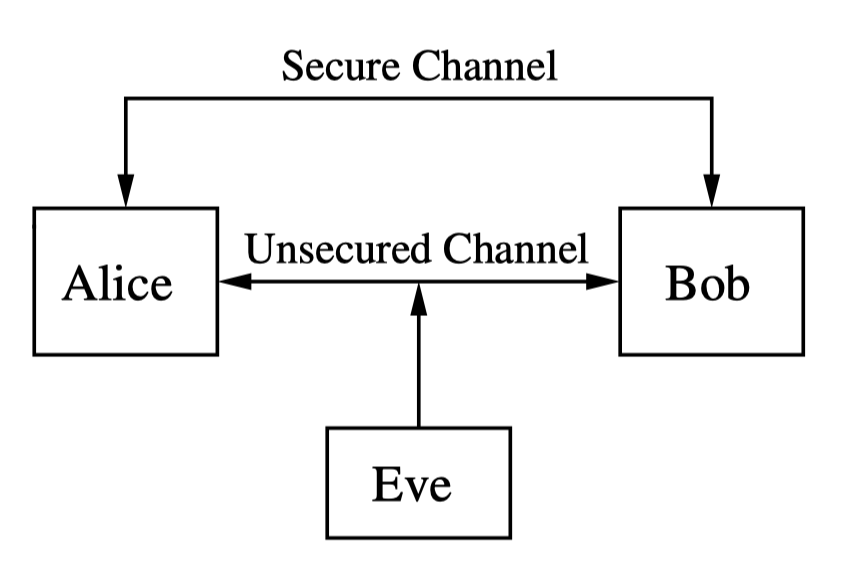
\includegraphics[width=\textwidth]{using_SKES.png}
		\caption{Use a SKES to Achieve Confidentiality}
	\end{figure}
\end{center}

\subsubsection{Security Definitions}
Computational Power of the Adversary: \begin{itemize}
\item Information-theoretic security: Eve has infinite computational resources.
\item Complexity-theoretic security: Eve is a ‘polynomial-time Turing machine’.
\item Computational security: Eve has 36,768 Intel E5-2683 V4 cores running at 2.1 GHz at her disposal.
\end{itemize}

Adversary’s Interaction: \begin{itemize}
\item Passive attacks\begin{itemize}
\item Ciphertext-only attack: The adversary knows some ciphertext (that was generated by Alice or Bob).
\item Known-plaintext attack: The adversary also knows some plaintext and the corresponding ciphertext.
\end{itemize}
\item Active attacks\begin{itemize}
\item Chosen-plaintext attack: The adversary can also choose some plaintext and obtains the corresponding ciphertext.
\end{itemize}
\item Other attacks\begin{itemize}
\item Clandestine attacks: bribery, blackmail, etc.
\item Side-channel attacks: monitor the encryption and decryption equipment (timing attacks, power analysis attacks, electromagnetic-radiation analysis, etc.)
\end{itemize}
\end{itemize}

Adversary’s Goal: \begin{itemize}
\item Recover the secret key.
\item Systematically recover plaintext from ciphertext (without necessarily learning the secret key).
\item Learn some partial information about the plaintext from the ciphertext (other than its length).
\end{itemize}

If the adversary can achieve 1 or 2, the SKES is said to be \textbf{totally insecure} (or \textbf{totally broken}).

If the adversary cannot learn any partial information about the plaintext from the ciphertext (except possibly its length), the SKES is said to be \textbf{semantically secure}.

\begin{definition}
	A symmetric-key encryption scheme is said to be \textbf{secure} if it is semantically secure against chosen- plaintext attack by a computationally bounded adversary.
\end{definition}

To break a symmetric-key encryption scheme, the adversary has to accomplish the following:
\begin{enumerate}
	\item The adversary is given a challenge ciphertext $c$ (generated by Alice or Bob using their secret key $k$).
	\item During its computation, the adversary can select plaintexts and obtains (from Alice or Bob) the corresponding ciphertexts.
	\item After a feasible amount of computation, the adversary obtains some information about the plaintext $m$ corresponding to the challenge ciphertext $c$ (other than the length of $m$).
\end{enumerate}

Desirable Properties of a SKES: \begin{enumerate}
\item Efficient algorithms should be known for computing $E_k$ and $D_k$ (i.e. for encryption and decryption).
\item The secret key should be small (but large enough to render exhaustive key search infeasible).
\item The scheme should be \textbf{secure}.
\item The scheme should be secure even against the designer of the system.
\end{enumerate}

\begin{definition}
	A cryptographic scheme is said to have a \textbf{security level} of $\ell$ bits if the fastest known attack on the scheme takes approximately $2^\ell$ operations.
	
	As of the year 2021, a security level of 128 bits is desirable in practice.
\end{definition}

\subsubsection{The Simple Substitution Cipher}
\begin{definition}
	The Simple Substitution Cipher is defined as follows: \begin{itemize}
	\item $M = $ all English messages. 
	\item $C =$ all encrypted messages. 
	\item $K = $ all permutations of the English alphabet. 
	\item $E_k (m)$: Apply permutation $k$ to $m$, one letter at a time. \item $D_k (c)$: Apply inverse permutation $k^{-1}$ to $c$, one letter at a time.
	\end{itemize}
\end{definition}

Clearly, it is totally insecure against a chosen-plaintext attack. 

For ciphertext-only attack: 
\begin{itemize}
	\item Given sufficient amounts of ciphertext $c$, decrypt $c$ using each possible key until $c$ decrypts to a plaintext message which ``makes sense''.
	\item In principle, 30 characters of ciphertext are sufficient on average to yield a unique plaintext that is a sensible English message. In practice, a few hundred characters are needed.
	\item In terms of exhaustive key search, the number of keys to try is $26! \approx 4\times 10^{26} \approx 2^{88}$
	\item If the adversary uses $10^6$ computers, each capable of trying $10^9$ keys per second, then exhaustive key search takes about $10^4$ years. So, exhaustive key search is infeasible.
	\item However, we can do a simple frequency analysis to break this scheme. 
\end{itemize}

\subsubsection{Work Factor}
\begin{definition}
	For this course, we consider: \begin{itemize}
	\item $2^{40}$ operations is considered \textbf{very easy}.
	\item $2^{56}$ operations is considered \textbf{easy}. 
	\item $2^{64}$ operations is considered \textbf{feasible}. 
	\item $2^{80}$ operations is considered \textbf{barely feasible}.
	\item $2^{128}$ operations is considered \textbf{infeasible}.
	\end{itemize}
\end{definition}

\begin{definition}
	The \textbf{Landauer limit} from thermodynamics suggests that exhaustively trying $2^{128}$ symmetric keys would require $\gg 3000$ gigawatts of power for one year (which is $\gg 100\%$  of the world’s energy production).
\end{definition}

\subsubsection{Polyalphabetic Ciphers}
Since the simple substitution cipher is totally broken even against ciphertext-only attacks, we can consider the following idea: use several permutations, so a plaintext letter is encrypted to one of several possible ciphertext letters

For example, \textbf{Vigenere cipher} encrypts in the following way: 
\begin{center}
	\begin{figure}[h!]
		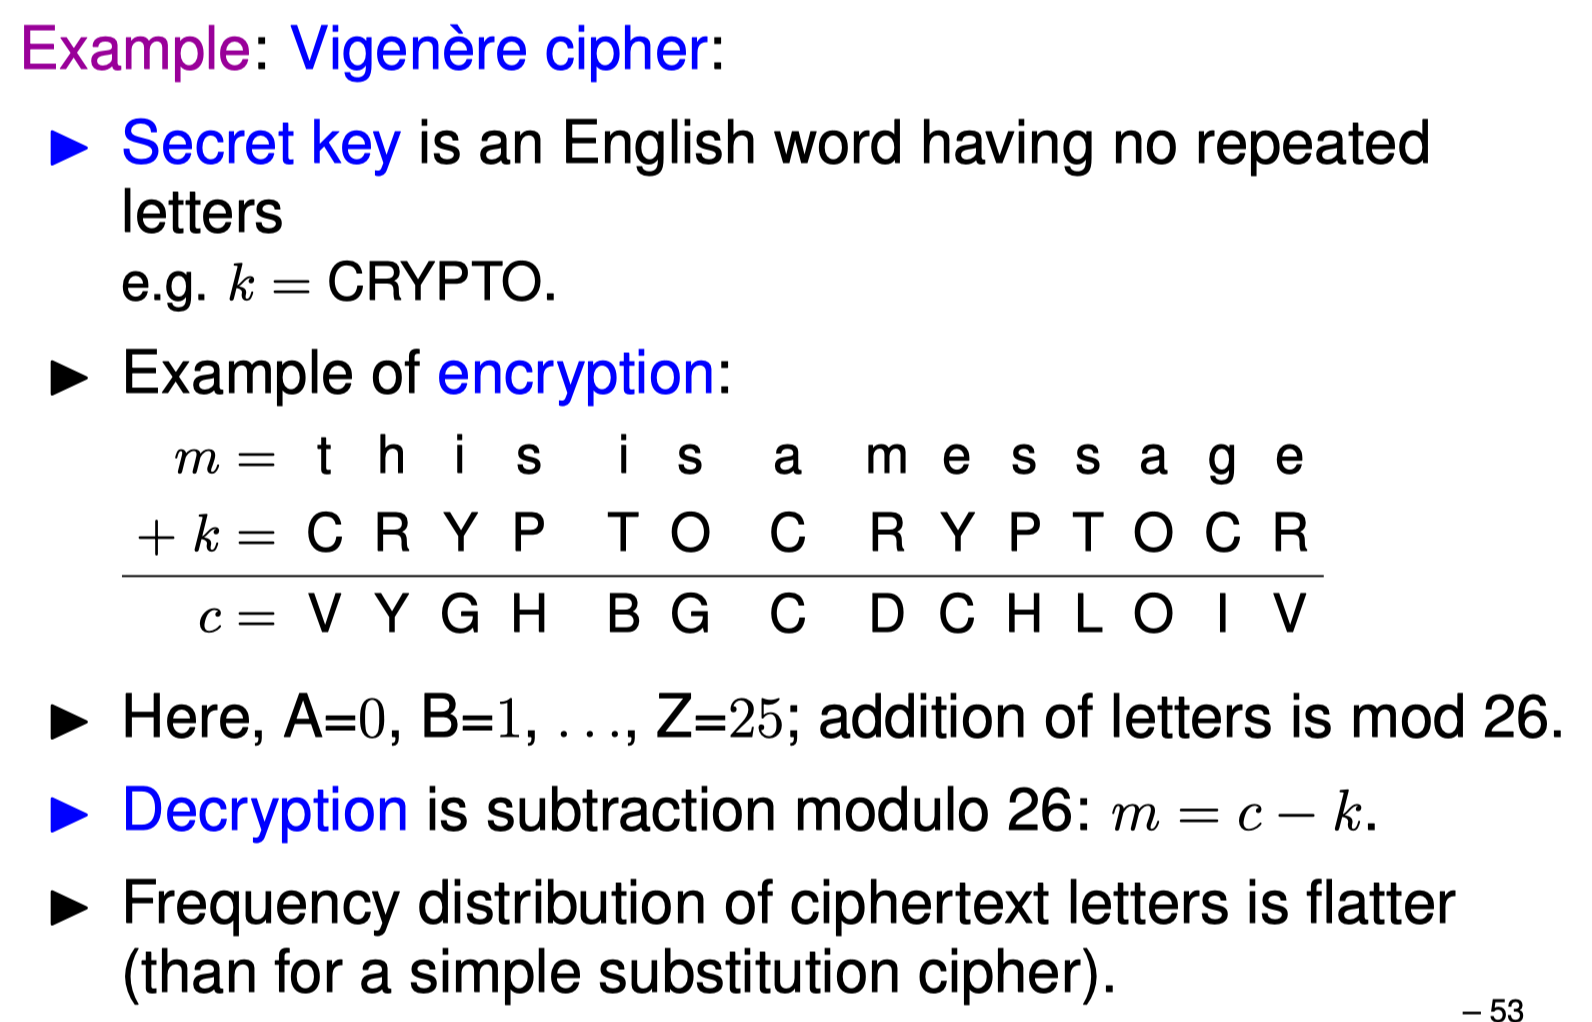
\includegraphics[width=\textwidth]{Vigenere_cipher.png}
		\caption{Vigenere Cipher}
	\end{figure}
\end{center}

However, it is still totally insecure under a chosen-plaintext attack or a ciphertext-only attack

\subsubsection{Convention and Notations}
\begin{itemize}
	\item From now on, unless otherwise stated, messages and keys will be assumed to be \textbf{bit strings}
	\item $\oplus$ is is bitwise exclusive-or (XOR), or equivalently, bitwise addition modulo 2.
\end{itemize}

\subsection{One Time Pad}
Using the idea from above, we can do a one-time pad, which is invented Vernam in 1917 for the telegraph system. The key a \textbf{random} string of letters, and the key is as long as the plaintext.
\begin{center}
	\begin{figure}[h!]
		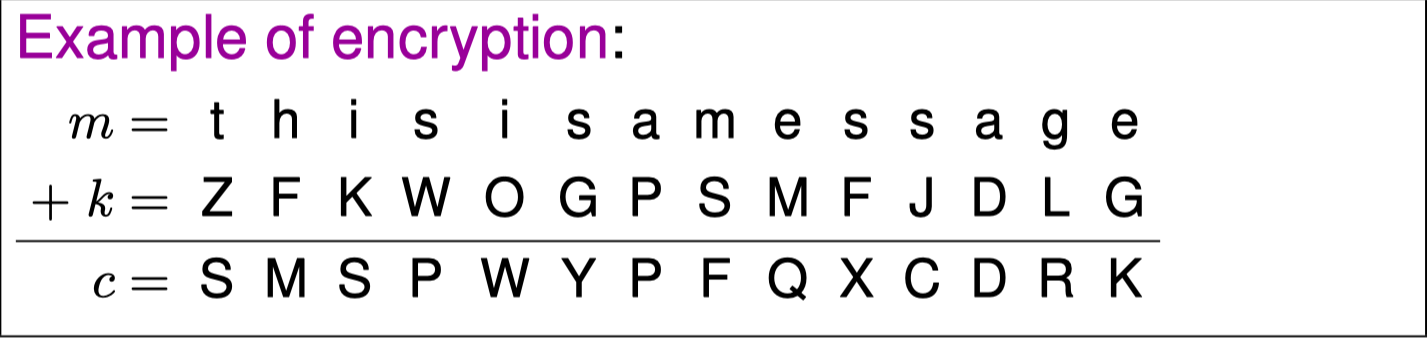
\includegraphics[width=\textwidth]{one_time_pad.png}
		\caption{Example of One Time Pad}
	\end{figure}
\end{center}

Note that The key should not be re-used: \begin{itemize}
\item If $c_1 = m_1 +k$ and $c_2 = m_2 +k$, then $c_1 -c_2 = m_1 -m_2$
\item Thus $c_1 -c_2$ depends only on the plaintext (and not on the key) and hence can leak information about the plaintext.
\item In particular, if $m_1$ is known, then $m_2$ can be easily computed.
\end{itemize}
The encryption of one-time pad would be $c = m \oplus k$, and decryption would be $m = c \oplus k$

\begin{definition}
	\textbf{Perfect secrecy}: The one-time pad is \textbf{semantically secure} against ciphertext-only attack by an adversary with infinite computational resources.
\end{definition}

Remarks: \begin{itemize}
\item This can be proven formally using concepts from information theory [Shannon 1949].
\item The bad news: Shannon (1949) proved that if plaintexts are $m$-bit strings, then any symmetric-key encryption scheme with perfect secrecy must have $|K| \geq 2^m$.
\item So, perfect secrecy (and the one-time pad) is fairly useless in practice.
\end{itemize}

\subsection{Stream Ciphers}
The basic idea is that instead of using a \textbf{random} key in the one-time pad, we can use a ``\textbf{pseudorandom}'' key. 

\begin{definition}
	A \textbf{pseudorandom bit generator (PRBG)} is a deterministic algorithm that takes as input a (random) \textbf{seed}, and outputs a longer ``\textbf{pseudorandom}'' sequence called the \textbf{keystream}.
\end{definition}

The security of this depends on the quality of the PRBG. We have several requirements on that: \begin{itemize}
\item The keystream should be ``indistinguishable'' from a random sequence (the \textbf{indistinguishability} requirement).
\item If an adversary knows a portion $c_1$ of ciphertext and the corresponding plaintext $m_1$ , then she can easily find the corresponding portion $k_1 = c_1 \oplus m_1$ of the keystream. Thus, given portions of the keystream, it should be \textbf{infeasible} to learn \textbf{any information} about the rest of the keystream (the \textbf{unpredictability} requirement).
\end{itemize}

\begin{center}
	\begin{figure}[h!]
		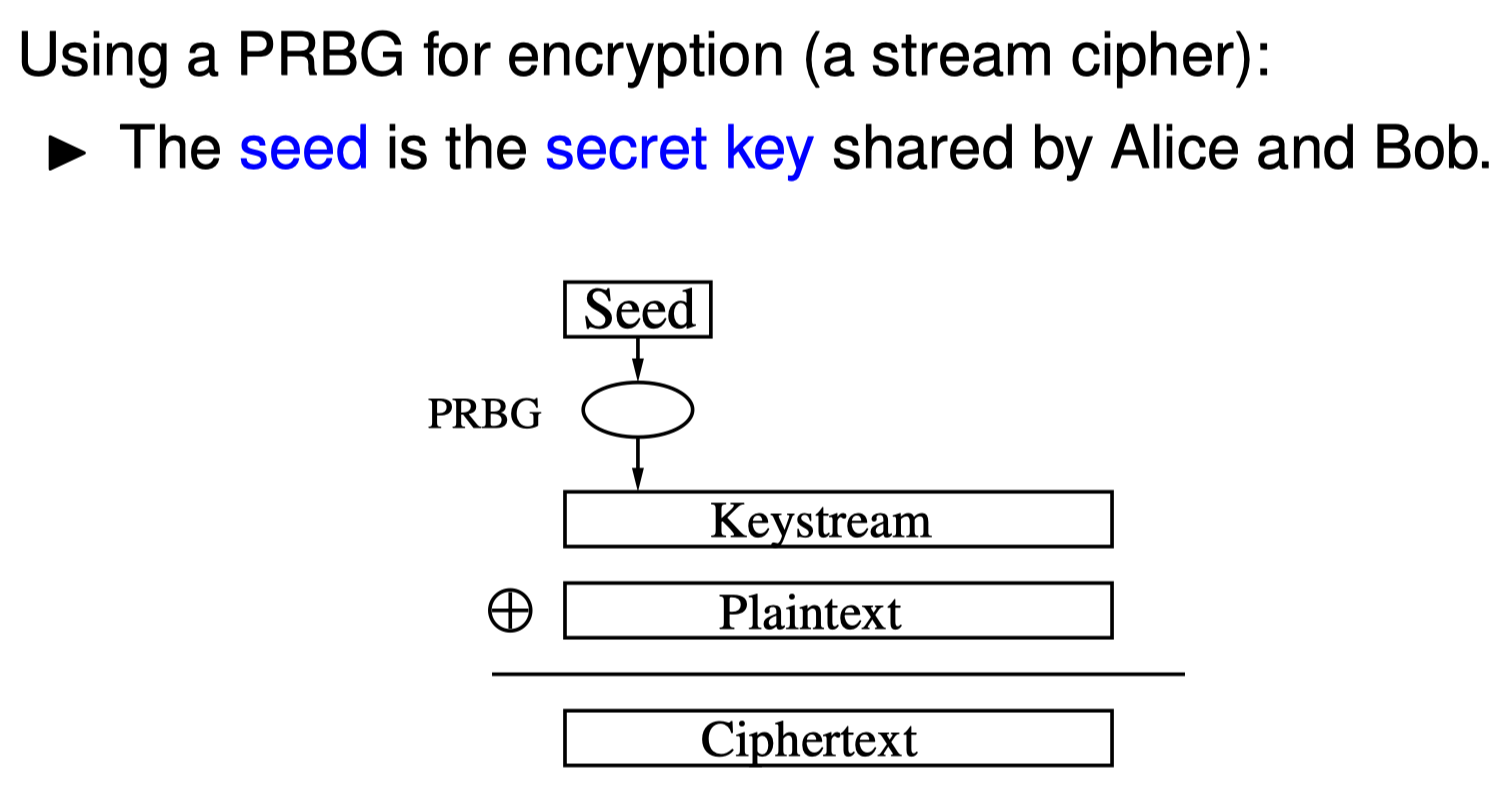
\includegraphics[width=\textwidth]{PRBG.png}
		\caption{Encryption of PRBG}
	\end{figure}
\end{center}

\subsection{The RC4 Stream Cipher}

It is designed by Ron Rivest in 1987: \begin{itemize}
\item Pros: Extremely simple; extremely fast; variable key length. No catastrophic weakness has been found.
\item Cons: Design criteria are proprietary; not much public scrutiny until the year 2001
\item RC4 has two components: (i) a \textbf{key scheduling algorithm}, and (ii) \textbf{a keystream generator}.
\end{itemize}

In the following, $K[i], \bar{K}[i]$ and $S[i]$ are 8-bit integers (bytes).

\begin{algorithm}[H]
	\KwInput{Secret key $K[0], K[1],..., K[d - 1]$. (Keylength is $8d$ bits.)}
	\KwOut{256-long array: $S[0], S[1], ..., S[255]$.}
	\For(){$i = 0$ to $255$}{
		$S[i] \leftarrow i$\\
		$\bar{K}[i] \leftarrow K[i \mod d]$
	}
	$K \leftarrow 0$\\
	\For(){$i = 0$ to $255$}{
		$j \leftarrow (\bar{K}[i] + S[i] + j) \mod 256$\\
		Swap ($S[i], S[j]$)
	}
	\caption{RC4 Key Scheduling Algorithm}
\end{algorithm}
The idea is that $S$ is a ``random-looking'' permutation of $\{0, 1, 2,..., 255\}$ that is generated from the secret key.

\begin{algorithm}[H]
	\KwInput{256-long byte array: $S[0], S[1], . . . , S[255]$ produced by the RC4 Key Scheduling Algorithm.}
	\KwOut{Keystream}
	$i \leftarrow 0$; $j \leftarrow 0$\\
	\While(){keystream bytes are required}{
		$i \leftarrow (i+1) \mod 256$\\
		$j \leftarrow (S[i] + j) \mod 256$\\
		Swap($S[i], S[j]$)\\
		$t \leftarrow (S[i] + S[j]) \mod 256$\\
		Output $S[t]$
	}
	\caption{RC4 Keystream Generator}
\end{algorithm}

For encryption, the keystream bytes are XORed with the plaintext bytes to produce ciphertext bytes.

\subsubsection{Wired Equivalent Privacy (WEP)}
It was ratified in September 1999. WEP’s goal is (only) to protect link-level data during wireless transmission between mobile stations and access points.

Main Security Goals of WEP: \begin{itemize}
\item \textbf{Confidentiality}: Prevent casual eavesdropping. Here, RC4 is used for encryption.
\item \textbf{Data Integrity}: Prevent tampering with transmitted messages. Here, An ``integrity checksum'' is used.
\item \textbf{Access Control}: Protect access to a wireless network infrastructure. Here, we discard all packets that are not properly encrypted using WEP.
\end{itemize}

Description of WEP Protocol: \begin{itemize}
\item Mobile stations share a secret key $k$ with access point: \begin{itemize}
\item $k$ is either 40 bits or 104 bits in length.
\item The standard does not specify how the key is to be distributed.
\item In practice, one shared key per LAN is common; this key is manually injected into each access point and mobile station; the key is not changed very frequently.
\end{itemize}
\item Messages are divided into \textbf{packets} of some fixed length (e.g. 1500 bytes).
\item WEP uses a per-packet 24-bit \textbf{initialization vector (IV)} $v$ to process each packet. WEP does not specify how the IVs are managed. In practice: \begin{itemize}
\item A random IV is generated for each packet; or
\item The IV is set to 0 and incremented by 1 for each use.
\end{itemize}
\end{itemize}

\begin{algorithm}[H]
	\caption{To send a packet $m$, an entity does the following}
	Select a 24-bit IV $v$\\
	Compute a 32-bit checksum: $S = CRC(m)$.\\
	\hskip2.0em 802.11 specifies that a CRC-32 checksum be used. CRC-32 is \textbf{linear}. That is, for any two messages $m_1$ and $m_2$ of the same bitlength, $CRC(m_1 \oplus m_2) = CRC(m_1) \oplus CRC(m_2)$.\\
	Compute $c = (m \| S) \oplus RC4(v \| k)$.\\
	\hskip2.0em $\|$ or $,$ denotes concatenation.\\
	\hskip2.0em $(v\|k)$ is the key used in the RC4 stream cipher\\
	Send $(v, c)$ over the wireless channel
\end{algorithm}

\begin{center}
	\begin{figure}[h!]
		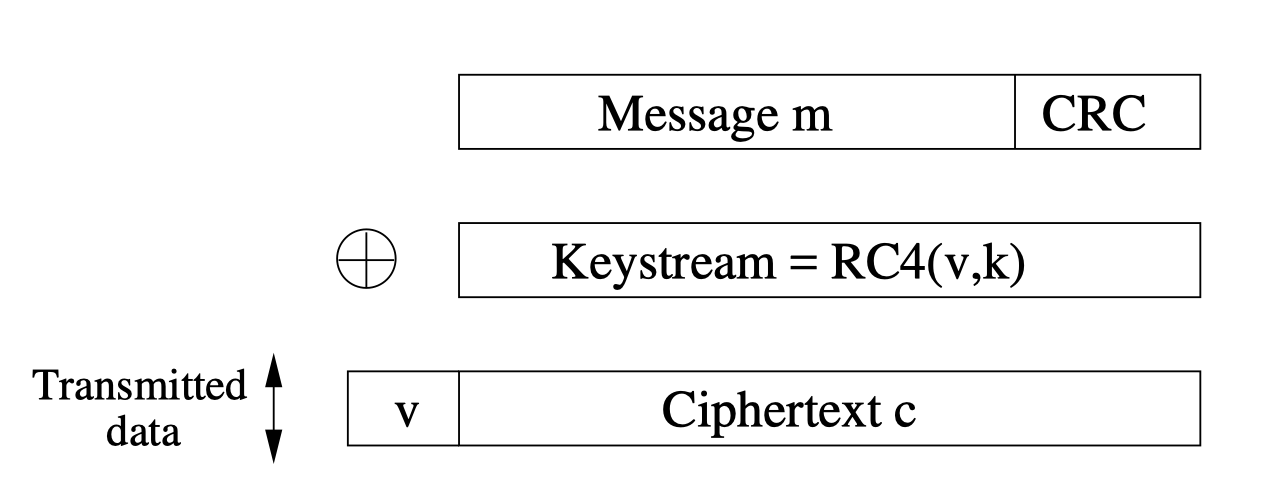
\includegraphics[width=\textwidth]{WEP_Protocol.png}
		\caption{Description of WEP Protocol}
	\end{figure}
\end{center}

\begin{algorithm}
	\caption{The receiver of $(v, c)$ does the following}
	Compute $(m \| S) = c \oplus RC4(v \| k)$.\\
	Compute $S' = CRC(m)$; reject the packet if $S' \neq S$.
\end{algorithm}

As proved by Borisov, Goldberg, and Wagner in 2021, none of confidentiality, data integrity, and access control are achieved. There are several problems: \begin{enumerate}
\item \textbf{IV Collision}: \begin{itemize}
\item Suppose that two packets $(v, c)$ and $(v, c')$ use the same IV $v$. Let $m, m'$ be the corresponding plaintexts. Then $c \oplus c' = (m \| S) \oplus (m' \| S')$. Thus, the eavesdropper can compute $m \oplus m'$.
\item If $m$ is known, then $m'$ is immediately available.
\item If $m$ is not known, then one may be able to use the expected distribution of $m$ and $m'$ to discover information about them. This is because some contents of network traffic is predictable.
\item To finding IV Collisions: \begin{itemize}
\item Since there are only $2^{24}$ choices for the IV, collisions are guaranteed after enough time — a few days on a busy network (5 Mbps).
\item If IVs are randomly selected, then one can expect a collision after about $2^{12}$ packets. This result comes from the birthday paradox. Suppose that an urn contains $n$ numbered balls. Suppose that balls are drawn from the urn, one at a time, with replacement. The expected number of draws before a ball is selected for a second time (called a \textbf{collision}) is approximately $\sqrt{\pi n/ 2} \approx \sqrt{n}$
\item Collisions are more likely if keys $k$ are long-lived and the same key is used for multiple mobile stations in a network.
\end{itemize}
\item So, WEP does not provide a high degree of confidentiality.
\end{itemize}
\item \textbf{Checksum is Linear}: \begin{itemize}
\item CRC-32 is used to check integrity. This is fine for random errors, but not for deliberate ones.
\item It is easy to make controlled changes to (encrypted) packets:\begin{itemize}
\item Suppose $(v, c)$ is an encrypted packet.
\item Let $c = RC4(v\|k) \oplus (m\|S)$, where $k, m, S$ are unknown.
\item Let $m' = m \oplus \Delta $, where $\Delta$ is a bit string. (The 1’s in $\Delta$ correspond to the bits of $m$ an attacker wishes to change.)
\item Let $c' = c \oplus (\Delta \| CRC(\Delta))$.
\item Then $(v, c')$ is a valid encrypted packet for $m'$.
\end{itemize}
\item So, WEP does not provide data integrity.
\end{itemize}
\item \textbf{Integrity Function is Unkeyed}: \begin{itemize}
\item Suppose that an attacker learns the plaintext $m$ corresponding to a single encrypted packet $(v, c)$.
\item Then, the attacker can compute the RC4 keystream $$RC4(v\|k) = c \oplus (m\|CRC(m))$$
\item Henceforth, the attacker can compute a valid encrypted packet for any plaintext $m'$ of her choice: $(v, c')$, where $c' = RC4(v\|k) \oplus (m'\|CRC(m'))$. 
\item So, WEP does not provide access control.
\end{itemize}
\end{enumerate}

\subsubsection{The Fluhrer-Mantin-Shamir Attack of WEP}
For this attack, we assume that: \begin{itemize}
\item The same 104-bit key $k$ is used for a long period of time. [Most products do this.]
\item The IV is incremented for each packet, or a random IV is selected for each packet. [Most products do this.]
\item The first plaintext byte of each packet (i.e. the first byte of each $m$) is known to the attacker.
[Most wireless protocols prepend the plaintext with some header bytes which are non-secret.]
\end{itemize}

To perform the attack, a passive adversary who can collect about 5,000,000 encrypted packets can very easily recover $k$ (and thus totally break the system).

In practice: \begin{itemize}
\item We can buy a \$100 wireless card and hack drivers to capture (encrypted) packets.
\item On a busy wireless network (5Mbps), 5 million packets can be captured in a few hours, and then $k$ can be immediately computed.
\end{itemize}

\subsubsection{Lessons Learned from WEP's Insecurity}
\begin{enumerate}
	\item \textbf{Details matter}: RC4 was considered to be a secure stream cipher. However, it was improperly used in WEP and the result was a highly insecure communications protocol. Do not assume that ``obvious'' ways of using cryptographic functions are secure.
	\item \textbf{Attacks only get better; they never get worse}: \begin{itemize}
	\item \textbf{Moore’s law (1965)}: computers get twice as fast every two years.
	\item Known attacks are constantly being tweaked and improved.
	\item New attacks are constantly being invented.
	\end{itemize}
	\item \textbf{Designing security is hard}:\begin{itemize}
	\item Designing cryptographic protocols is complicated and difficult.
	\item Clearly state your security objectives.
	\item Hire cryptography experts to design your security. Programming or engineering experts are not good enough.
	\item Make your protocols available for public scrutiny.
	\end{itemize}
	\item \textbf{There is a big demand in industry for ``security engineers''}: \begin{itemize}
	\item People who have a \textbf{deep understanding of applied cryptography} and have \textbf{excellent programming skills}.
	\end{itemize}
\end{enumerate}

\subsection{ChaCha20 Stream Cipher}
The \textbf{ChaCha20 stream cipher} is conceptually simple, word-oriented, and uses only simple arithmetic operations (integer addition modulo 2 32 , xor, and left rotations). It is designed by Dan Bernstein in 2008. It is extremely fast in software, and does not require any special hardware. To date, no security weaknesses have been found.
\begin{center}
	\begin{figure}[h!]
		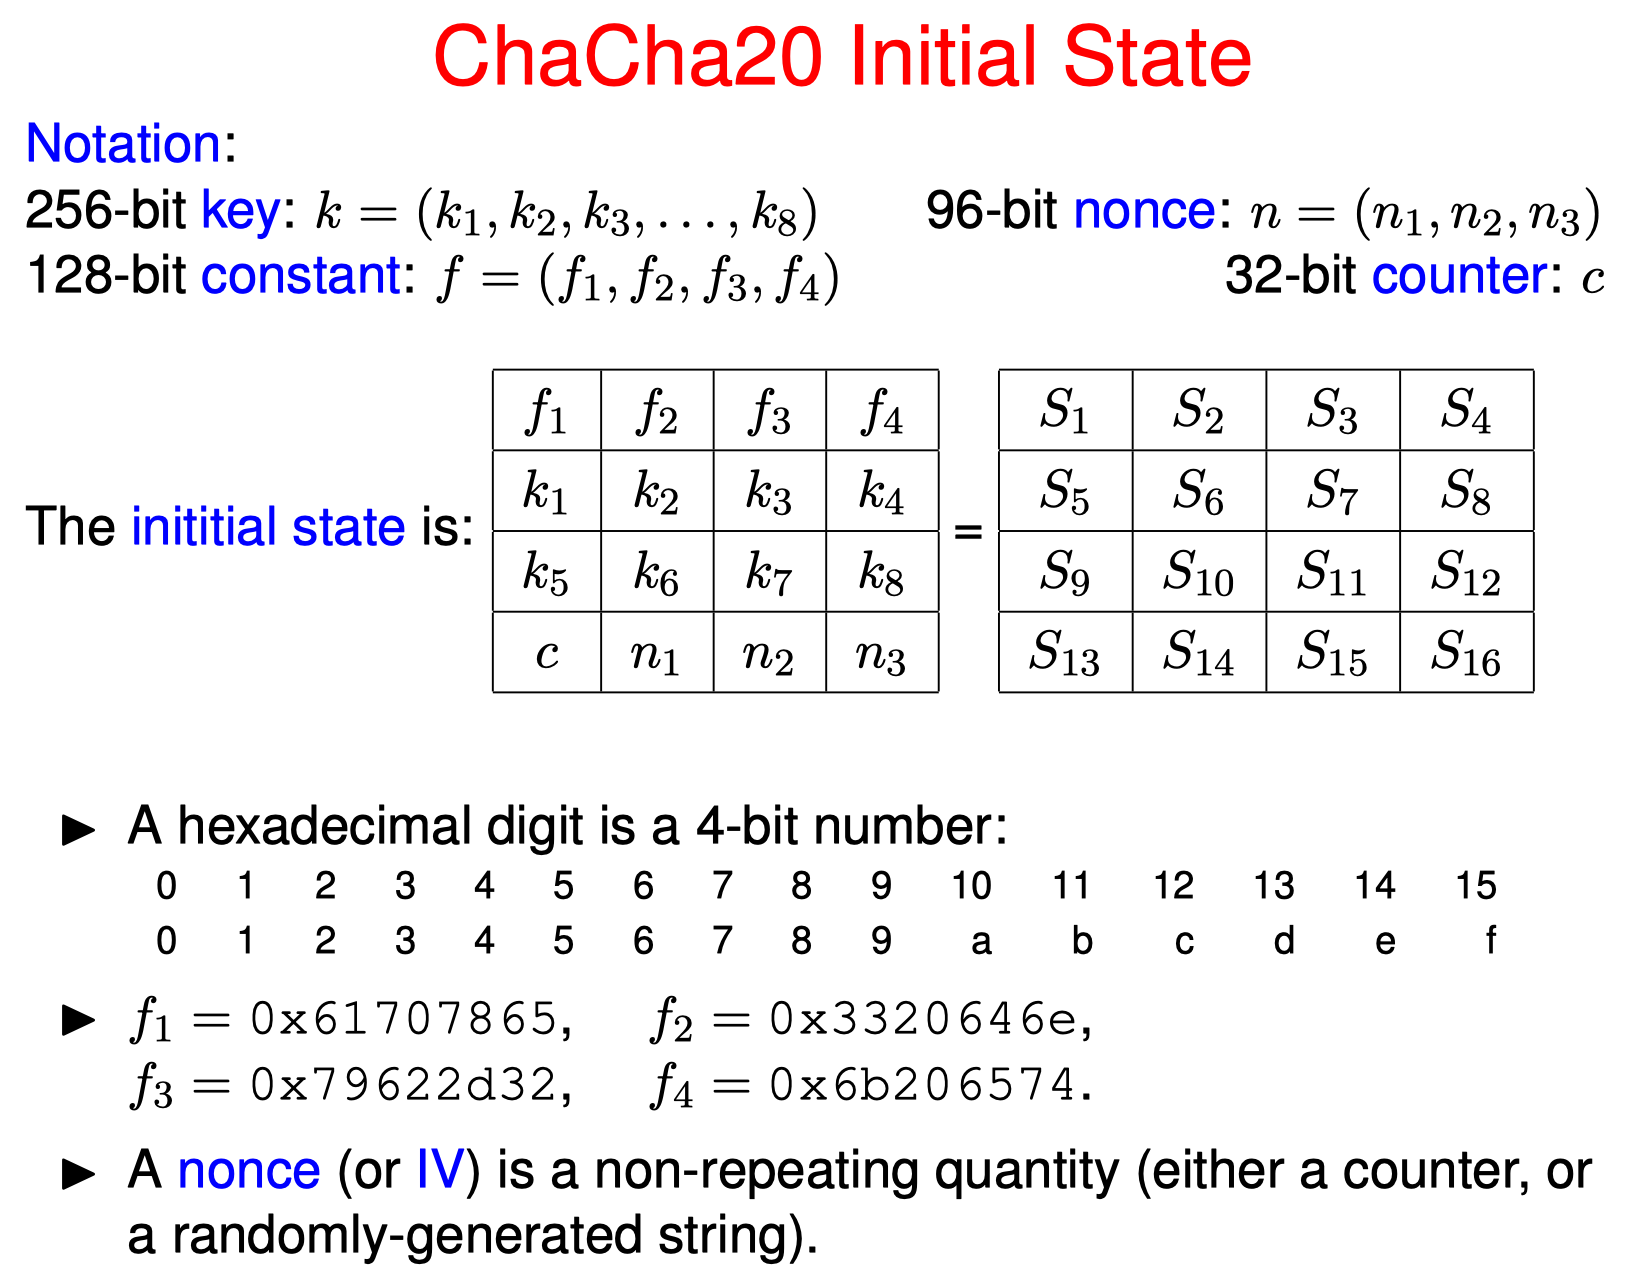
\includegraphics[width=\textwidth]{ChaCha20_Initial.png}
		\caption{ChaCha20 Initial State}
	\end{figure}
\end{center}
\newpage
\begin{center}
	\begin{figure}[h!]
		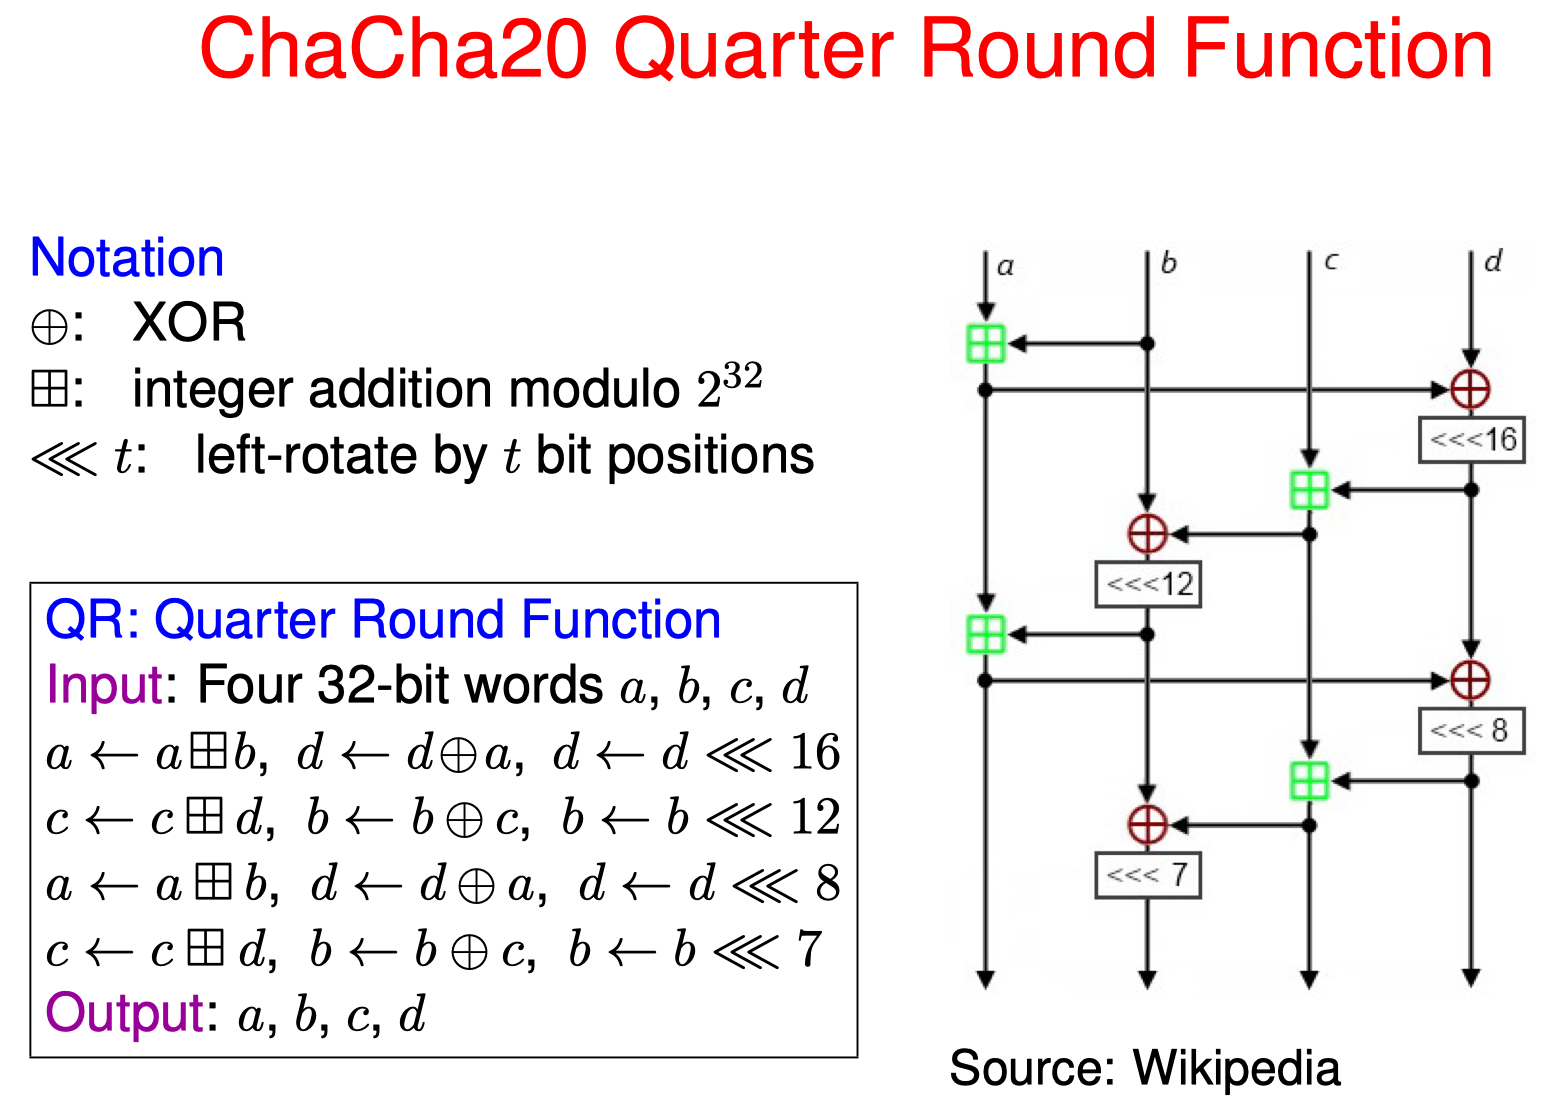
\includegraphics[width=\textwidth]{ChaCha20_quarter_round.png}
		\caption{ChaCha20 Quarter Round Function}
	\end{figure}
\end{center}
\newpage
\begin{algorithm}
	Select a nonce $n$ and initialize the counter $c$\\
	\While(){keystream bytes are required}{
		Create the initial state $S$\\
		Make a copy $S'$ of $S$\\
		Update $S$ by repeating the following 10 times: \\
		\hskip2.0em $QR(S_{1}, S_{5}, S_{9}, S_{13})$\\
		\hskip2.0em $QR(S_{2}, S_{6}, S_{10}, S_{14})$\\
		\hskip2.0em $QR(S_{3}, S_{7}, S_{11}, S_{15})$\\
		\hskip2.0em $QR(S_{4}, S_{8}, S_{12}, S_{16})$\\
		\hskip2.0em $QR(S_{1}, S_{6}, S_{11}, S_{16})$\\
		\hskip2.0em $QR(S_{2}, S_{7}, S_{12}, S_{13})$\\
		\hskip2.0em $QR(S_{3}, S_{8}, S_{9}, S_{14})$\\
		\hskip2.0em $QR(S_{4}, S_{5}, S_{10}, S_{15})$\\
		Output $S \oplus S'$ (64 keystream bytes).\\
		Increment the counter.
	}
	\caption{ChaCha20 Keystream Generator}
\end{algorithm}

For encryption, the keystream bytes are XORed with the plaintext bytes to produce ciphertext bytes. The nonce is included in the ciphertext.

\subsection{Block Ciphers}
\begin{definition}
	A \textbf{block cipher} is a SKES that breaks up the plaintext into blocks of a fixed length (e.g. 128 bits), and encrypts the blocks one at a time.
	
	In contrast, a stream cipher encrypts the plaintext one character (usually a bit) at a time.
\end{definition}

The Data Encryption Standard (DES): \begin{itemize}
\item Key length: 56 bits 
\item Block length: 64 bits
\item Size of key space: $2^{56}$
\end{itemize}

\begin{center}
	\begin{figure}[h!]
		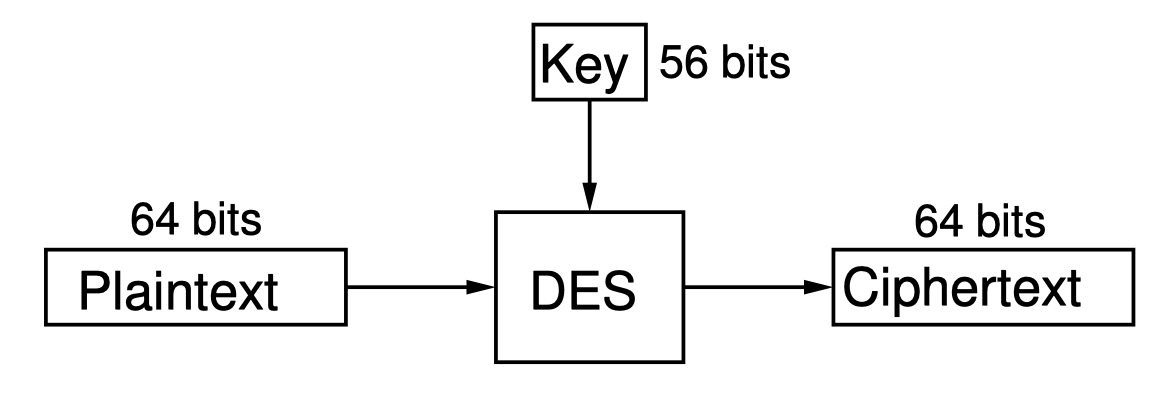
\includegraphics[width=\textwidth]{DES.png}
		\caption{Data Encryption Standard (DES)}
	\end{figure}
\end{center}

Some Desirable Properties of Block Ciphers (Design principles described by Claude Shannon in 1949): \begin{itemize}
\item Security: \begin{itemize}
\item \textbf{Diffusion}: each ciphertext bit should depend on all plaintext bits.
\item \textbf{Confusion}: the relationship between key and ciphertext bits should be complicated.
\item \textbf{Key length}: should be small, but large enough to preclude exhaustive key search.
\end{itemize}
\item Efficiency: \begin{itemize}
\item Simplicity (easier to implement and analyze).
\item High encryption and decryption rate.
\item Suitability for hardware or software.
\end{itemize}
\end{itemize}

DES has several problems: \begin{enumerate}
\item \textbf{Small Key Size}: \begin{itemize}
\item Exhaustive search on key space takes $2^{56}$ steps and can be easily parallelized
\item DES challenges from RSA Security (3 known PT/CT pairs): \begin{itemize}
\item June 1997: Broken in 3 months by Internet search. 
\item 1999: Broken in 56 hours by DeepCrack machine (1800 chips; \$250,000). 
\item 2006 Broken in 153 hours by COPACOBANA machine (\$10,000). \item 2012 Broken in 11.5 hours by crack.sh (\$200).
\end{itemize}
\item RC5 64-bit challenge: \begin{itemize}
\item July 2002: Broken in 1757 days.
\item Participation by 331,252 individuals.
\end{itemize}
\end{itemize}
\item \textbf{Small Block Size}: \begin{itemize}
\item If plaintext blocks are distributed ``uniformly at random'', then the expected number of ciphertext blocks observed before a collision occurs is $\approx 2^{32}$ (by the birthday paradox). Hence the ciphertext reveals \textbf{some} information about the plaintext.
\item Small block length is also damaging to some authentication applications
\end{itemize}
\end{enumerate}

\subsubsection{Double-DES}
Since the only (substantial) weaknesses known in DES are the obvious ones: small key length and small block length, we may consider perform multiple encryption on DES. 

For Double-DES: \begin{itemize}
\item The key is $k = (k_1, k_2), k_1, k_2 \in_R \{0, 1\}^{56}$. 
	
[$k \in_R K$ means that $k$ is chosen \textbf{uniformly} and \textbf{independently} \textbf{at random} from $K$]
\item Encryption: $c = E_{k_2} (E_{k_1} (m))$, in which ($E$ = DES encryption, $E^{-1}$ = DES decryption)
\item Decryption: $m = E_{k_1}^{-1} (E_{k_2}^{-1} (c))$.
\item The Double-DES key length is $\ell = 112$, so exhaustive key search takes $2^{112}$ steps (infeasible).
\item Note that Block length is unchanged.
\end{itemize}

\begin{center}
	\begin{figure}[h!]
		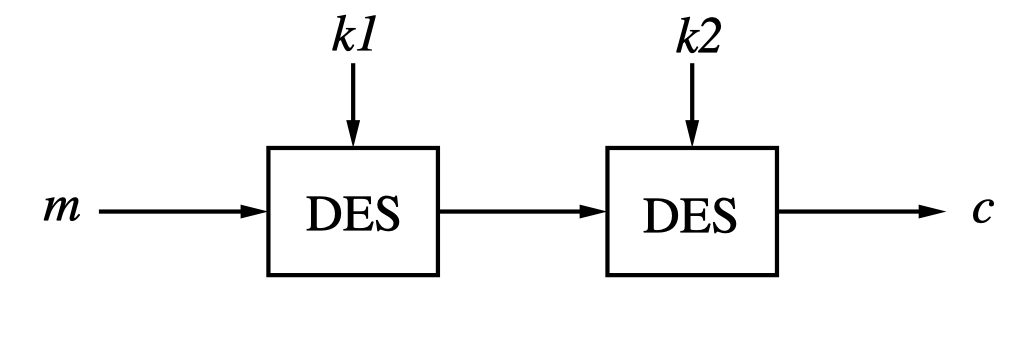
\includegraphics[width=\textwidth]{Double_DES.png}
		\caption{Double-DES Encryption}
	\end{figure}
\end{center}

However, we can attack Double DES in a more efficient way. The main idea is to see that $$c = E_{k_2} (E_{k_1} (m)) \Leftrightarrow E_{k_2}^{-1} (c) = E_{k_1} (m)$$
\newpage
\begin{algorithm}
	\caption{Meet-In-The-Middle Attack on Double-DES}
	\KwIn{3 known PT/CT pairs $(m_1, c_1), (m_2, c_2), (m_3, c_3)$}
	\KwOut{The secret key $(k_1, k_2)$}
	\For(){each $h_2 \in \{0,1\}^{56}$}{
		Compute $E_{h_2}^{-1} (c_1)$, and store $[E_{h_2}^{-1}(c_1), h_2]$ in a table sorted by first component.
	}
	\For(){each $h_1 \in \{0,1\}^{56}$}{
		Compute $E_{h_1} (m_1)$\\
		Search for $E_{h_1} (m_1)$ in the table. (We say that $E_{h_1} (m_1)$ matches table entry $[E_{h_2}^{-1}(c_1), h_2]$ if $E_{h_2}^{-1}(c_1) = E_{h_1}(m_1)$\\
		\For(){each match $[E_{h_2}^{-1}(c_1), h_2]$ in the table}{
			\If(){$E_{h_2}(E_{h_1}(m_2)) = c_2)$}{
				\If(){$E_{h_2}(E_{h_1}(m_3)) = c_3$}{
					Output $(h_1, h_2)$ and STOP
				}
			}
		}
	}
\end{algorithm}

Analysis on this algorithm: \begin{itemize}
\item First, see how to calculate $FK$ in the following section. 
\item Let $E$ be the DES encryption function, so Double-DES encryption is $c = E_{k_2} (E_{k1} (m))$.
\item If $\ell = 112, L = 64, t=3$, then $FK \approx 1/2^{80} \approx 0$
Thus if a Double-DES key $(h_1 , h_2)$ is found for which $E_{h_2}(E_{h_1}(m_i)) = c_i$ for $i = 1, 2, 3$, then with very high probability we have $(h_1 , h_2 ) = (k_1 , k_2)$.
\item If $\ell = 112, L = 64, t=1$, then $FK \approx 2^{48}$. Thus the expected number of Double-DES keys $(h_1 , h_2 )$ for which $E_{h_2}(E_{h_1}(m_1)) = c_1$ is $\approx 2^{48}$.
\item If $\ell = 112, L = 64, t=2$, then $FK \approx 1/2^{16}$. Thus the expected number of Double-DES keys $(h_1 , h_2 )$ for which $E_{h_2}(E_{h_1}(m_1)) = c_1$ and $E_{h_2}(E_{h_1}(m_2)) = c_2$ is $\approx 2^{-16}$.
\item So, the number of DES operations is $\approx 2^{56} + 2^{56} + 2 \cdot 2^{48} \approx 2^{57}$
\item Space requirements: $2^{56} (64 + 56)$ bits $\approx 1,080,863 $ Tbytes.
\end{itemize}

\textbf{Time-memory tradeoff}: The attack can be modified to decrease the storage requirements at the expense of time:\begin{itemize}
\item Time: $2^{56+s}$ steps
\item memory: $2^{56-s}$ units
\item $1 \leq s \leq 55$.
\end{itemize}

\subsubsection{False Keys}
What is the number of known plaintext/ciphertext pairs needed for unique key determination? 

Let's formulate this question in the following way: 
Let $E$ be a block cipher with key space $K = \{0, 1\}^\ell $, and plaintext and ciphertext space $\{0, 1\}^L$.

Let $k' \in K$ be the secret key chosen by Alice and Bob, and let $(m_i , c_i)$, $1 \leq i \leq t$, be known plaintext/ciphertext pairs, where the plaintext $m_i$ are distinct.

(Note that $c_i = E_{k'}(m_i)$ for all $1 \leq i \leq t$)

Then how large should $t$ be to ensure (with probability very close to 1) that there is only one key $k \in K$ such that $E_k (m_i) = c_i$ for all $1 \leq i \leq t$?

The simple answer is that select $t$ such that $FK \approx 0$

How do we calculate $FK$? \begin{itemize}
\item For each $k \in K$, the encryption function $E_k : \{0, 1\}^L \rightarrow \{0, 1\}^L$ is a permutation.
\item We make the \textbf{heuristic} assumption that for each $k \in K$, $E_k$ is a random function (i.e., a randomly selected function). This assumption is certainly false since $E_k$ is not random, and because a random function is almost certainly not a permutation. Nonetheless, it turns out that the assumption is good enough for our analysis.
\item Now, fix $k \in K$, $k \neq k'$. Then the probability that $E_k(m_i) = c_i$ for all $1 \leq i \leq t$ is $$\underbrace{\frac{1}{2^L}\cdot\frac{1}{2^L}\cdots \frac{1}{2^L}}_{t} = \frac{1}{2^{Lt}}$$
\item Thus the expected number of \textbf{false keys} $k \in K$ (not including $k'$) for which $E_k(m_i) = c_i$ for all $1 \leq i \leq t$ is $$FK = \frac{2^\ell -1}{2^{Lt}}$$
\end{itemize}

\subsubsection{Storage Units}
\begin{itemize}
	\item $10^3$ bytes = 1 Kbyte (kilo) $\approx 2^{10}$ bytes
	\item $10^3$ Kbyte = 1 Mbyte (mega) $\approx 2^{20}$ bytes
	\item $10^3$ Mbyte = 1 Gbyte (giga) $\approx 2^{30}$ bytes
	\item $10^3$ Gbyte = 1 Tbyte (tera) $\approx 2^{40}$ bytes
	\item $10^3$ Tbyte = 1 Pbyte (peta) $\approx 2^{50}$ bytes
	\item $10^3$ Pbyte = 1 Ebyte (exa) $\approx 2^{60}$ bytes
\end{itemize}

\subsubsection{Triple-DES}

Since: \begin{itemize}
\item Double-DES has the same effective key length as DES.
\item Double-DES is not much more secure than DES.
\end{itemize}

We can consider have Triple-DES: \begin{itemize}
\item Key is $k = (k_1 , k_2 , k_3 )$, $k_1, k_2, k_3 \in_R \{0, 1\}^{56}$
\item Encryption: $c = E_{k_3} (E_{k_2} (E_{k_1} (m)))$, in which ($E =$ DES encryption, $E^{-1}$ = DES decryption)
\item Decryption: $m = E_{k_1}^{-1}(E_{k_2}^{-1} (E_{k_3}^{-1}(c)))$.
\item Key length of Triple-DES is $\ell = 168$, so exhaustive key search takes $2^{168}$ steps (infeasible).
\item Meet-in-the-middle attack takes $\approx 2^{112}$ steps.
\item So, the effective key length of Triple-DES against exhaustive key search is $\approx 112$ bits.
\end{itemize}

\begin{center}
	\begin{figure}[h!]
		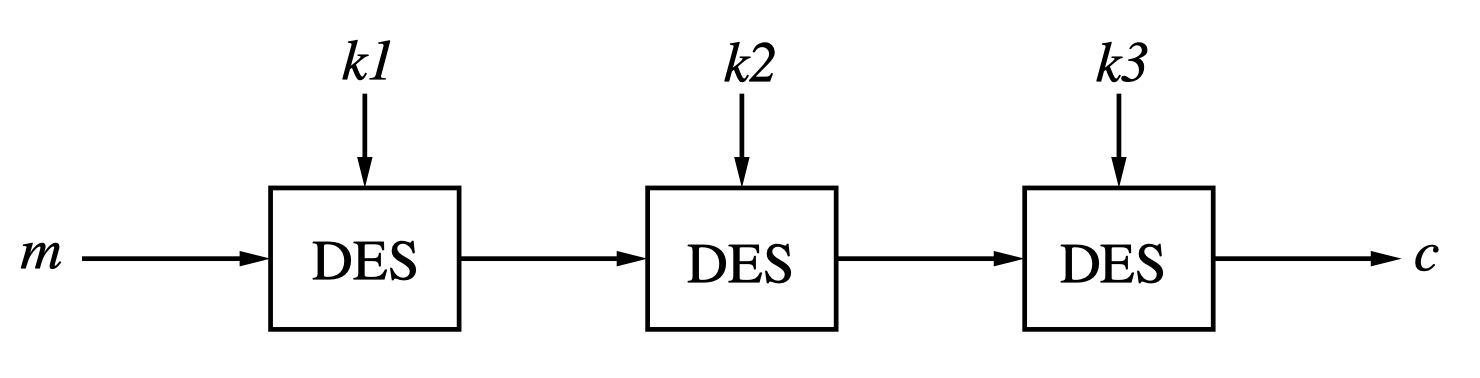
\includegraphics[width=\textwidth]{Triple_DES.png}
		\caption{Triple DES Encryption}
	\end{figure}
\end{center}
\newpage
\subsection{The Advanced Encryption Standard (AES)}
\begin{itemize}
	\item Key lengths: 128, 192 and 256 bits. 
	\item Block length: 128 bits. 
	\item Efficient on both hardware and software platforms. 
	\item Availability on a worldwide, non-exclusive, royalty-free basis.
\end{itemize}
\begin{center}
	\begin{figure}[h!]
		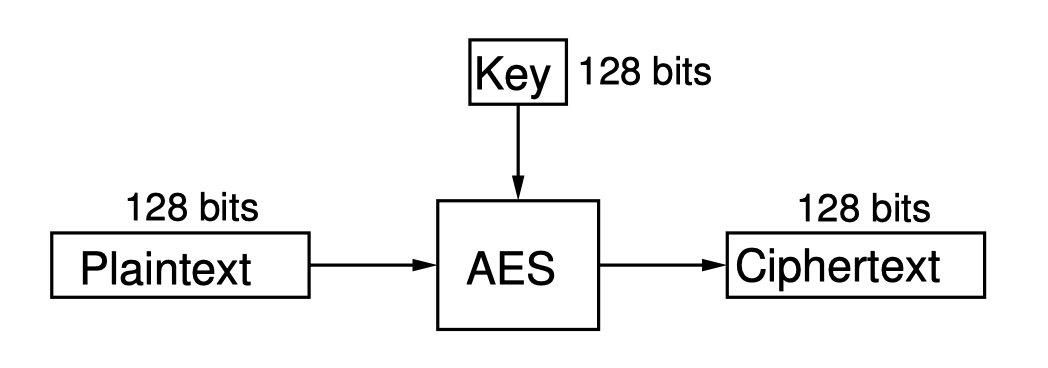
\includegraphics[width=\textwidth]{AES.png}
		\caption{AES Encryption}
	\end{figure}
\end{center}

\begin{definition}
	A \textbf{substitution-permutation network (SPN)} is an iterated block cipher where a round consists of a \textbf{substitution} operation followed by a \textbf{permutation} operation.
	
	Components of a SPN cipher: \begin{itemize}
	\item $n$: block length
	\item $\ell$: key length
	\item $h$: the number of rounds
	\item A fixed invertible function $S: \{0, 1\}^b \rightarrow \{0,1\}^b$, where b is a divisor of $n$
	\item A fixed permutation $P$ on $\{1, 2, ..., n\}$
	\item A key scheduling algorithm that determines subkeys $k_1, k_2, ..., k_h , k_{h+1}$ from a key $k$
	\end{itemize}
\end{definition}

Note: $n, \ell, h, S, P$ and the key scheduling algorithm are public. The only secret in AES is the key $k$ that is selected.

\begin{algorithm}
	\caption{SPN Encryption}
	$A \leftarrow $ plaintext\\
	\For(){$i = 1 ... h$}{
		$A \leftarrow A \oplus k_i$ (XOR)\\
		$A \leftarrow S(A)$ (Substitution)\\
		$A \leftarrow P(A)$ (Permutation)\\
	} 
	$A \leftarrow A \oplus k_{h+1}$\\
	ciphertext $\leftarrow A$
\end{algorithm}

\begin{center}
	\begin{figure}[h!]
		\centering
		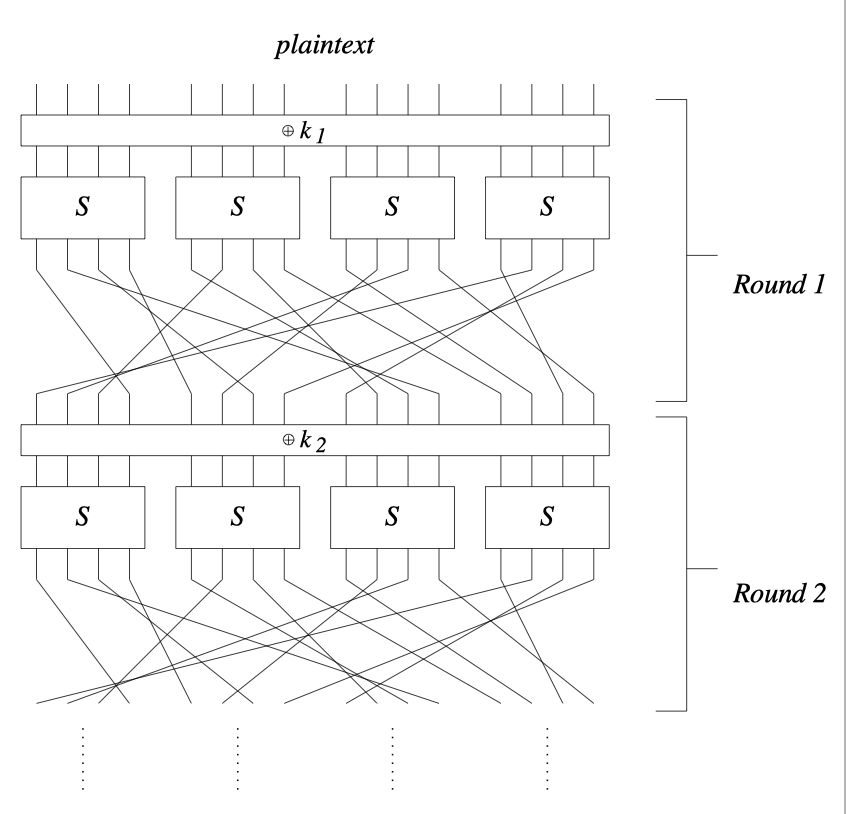
\includegraphics[width=0.5\textwidth]{SPN.png}
		\caption{SPN Encryption}
	\end{figure}
\end{center}

Decryption is just the reverse of encryption.

\begin{itemize}
	\item AES is an SPN, where the permutation operation is replaced by two invertible linear transformations.
	\item All operations are \textbf{byte} oriented (e.g., $b = 8$ so the S-box maps 8-bits to 8-bits). This allows AES to be efficiently implemented on software platforms.
	\item The \textbf{block length} of AES is $n = 128$ bits.
	\item Each \textbf{subkey} is 128 bits.
	\item AES accepts three different key lengths. The number of rounds $h$ depends on the key length:
\end{itemize}
\begin{center}
	\begin{tabular}{|c|c|c|}
		\hline
		cipher  & key length $\ell$ & $h$ \\
		\hline
		AES-128 & 128               & 10  \\
		AES-192 & 192               & 12  \\
		AES-256 & 256               & 14  \\
		\hline
	\end{tabular}
\end{center}

AES Round Operations: \begin{itemize}
\item Each round updates a variable called \textbf{State} which consists of a $4 \times 4$ array of bytes (note: $4 \times 4 \times 8 = 128$, the block length). 
\item \textbf{State} is initialized with the plaintext: \begin{center}
\begin{tabular}{|c|c|c|c|}
	\hline
	$a_{0, 0}$ & $a_{0, 1}$ & $a_{0, 2}$ & $a_{0, 3}$ \\
	\hline
	$a_{1, 0}$ & $a_{1, 1}$ & $a_{1, 2}$ & $a_{1, 3}$ \\
	\hline
	$a_{2, 0}$ & $a_{2, 1}$ & $a_{2, 2}$ & $a_{2, 3}$ \\
	\hline
	$a_{3, 0}$ & $a_{3, 1}$ & $a_{3, 2}$ & $a_{3, 3}$ \\
	\hline
\end{tabular} $ \leftarrow $ plaintext
\end{center}
\item After $h$ rounds are completed, a final subkey is XOR-ed with \textbf{State}, the result being the ciphertext.
\item The AES round function uses four \textbf{invertible} operations:\begin{enumerate}
\item \texttt{AddRoundKey} (key mixing). This step is bitwise-XOR each byte of \textbf{State} with the corresponding byte of the subkey.
\begin{center}
	\begin{figure}[h!]
		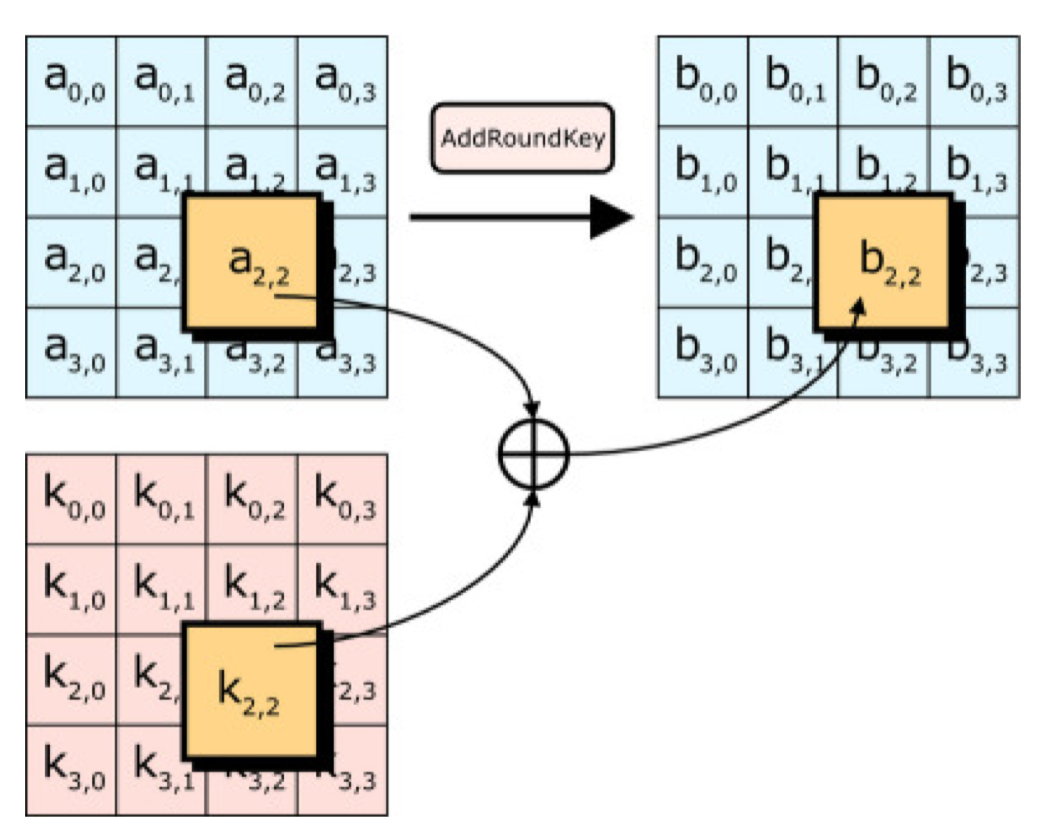
\includegraphics[width=\textwidth]{AES_Add_Round_Key.png}
		\caption{AES Add Round Key}
	\end{figure}
\end{center}
\item \texttt{SubBytes} (S-box). This step is take each byte in \textbf{State} and replace it with the output of the S-box. Here, $S : \{0, 1\}^8 \rightarrow \{0, 1\}^8$ is a fixed, public, invertible, and non-linear function.
\begin{center}
	\begin{figure}[h!]
		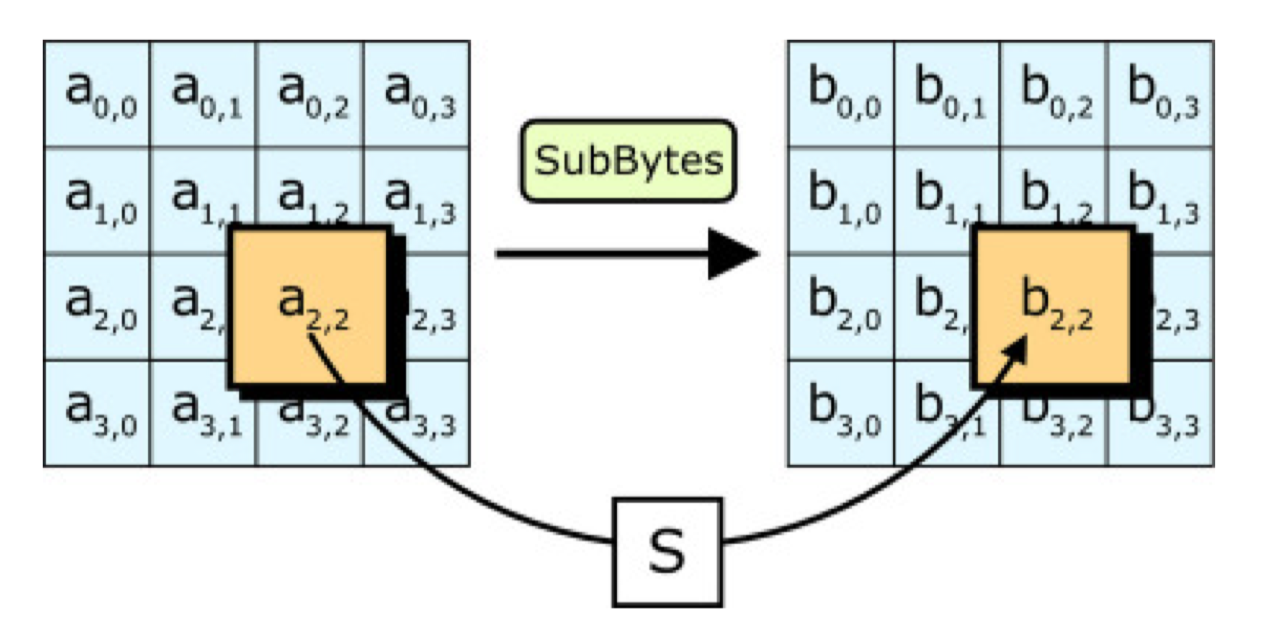
\includegraphics[width=\textwidth]{AES_Substitute_Bytes.png}
		\caption{AES Substitute Bytes}
	\end{figure}
\end{center}
\item \texttt{ShiftRows} (permutation). This step is permute the bytes of State by applying a \textbf{cyclic shift} to each row
\begin{center}
	\begin{figure}[h!]
		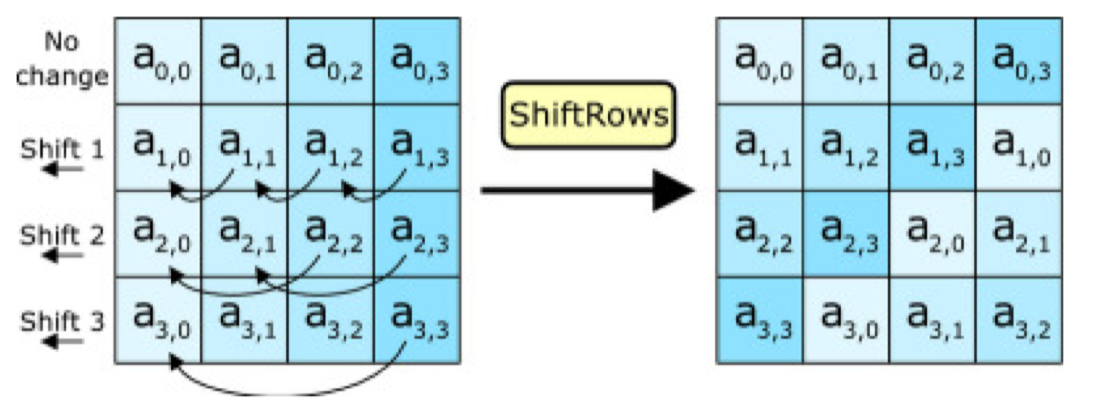
\includegraphics[width=\textwidth]{AES_Shift_Rows.png}
		\caption{AES Shift Rows}
	\end{figure}
\end{center}
\item \texttt{MixColumns} (linear transformation). 
\begin{center}
	\begin{figure}[h!]
		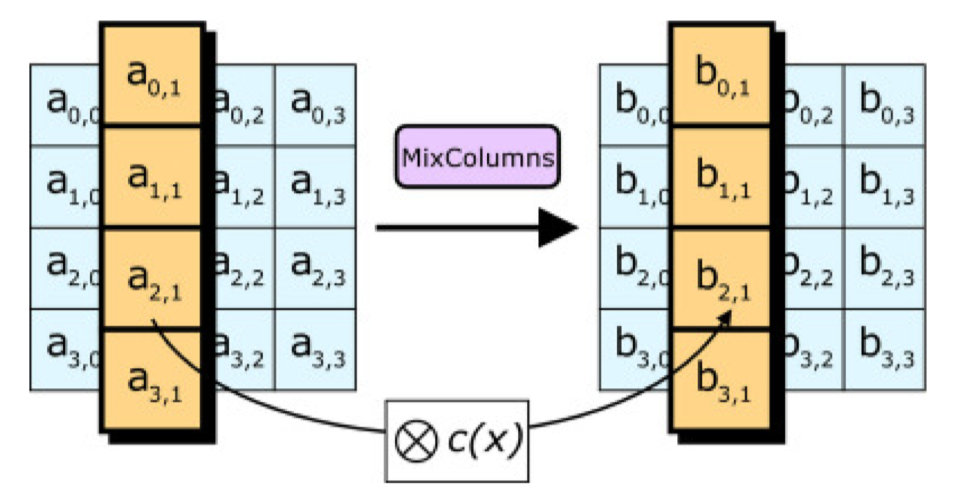
\includegraphics[width=\textwidth]{AES_Mix_Columns.png}
		\caption{AES Mix Columns}
	\end{figure}
\end{center}
\end{enumerate}
\end{itemize}
\subsubsection{Operation of AES}
Below we show some detailed explanation on the above operations. First, we need to define 
\begin{definition}
	The Finite Field $GF(2^8)$: The elements of the finite field $GF(2^8)$ are the polynomials of degree at most 7 in $\mathbb{Z}_2[y]$, with addition and multiplication performed modulo the irreducible polynomial $f(y) = y^8 + y^4 + y^3 + y + 1$.
	
	Then, we interpret an 8-bit string $a = a_7 a_6 a_5 a_4 a_3 a_2 a_1 a_0$ as coefficients of the polynomial $a(y) = a_7 y^7 + a_6 y^6 + a_5 y^5 + \cdots + a_1 y + a_0$ , and vice versa.
	
	We define the following operations: \begin{itemize}
	\item \textbf{Addition}: add coefficients with respect to each power of $y$. Perform modulo 2 on addition. 
	\item \textbf{Multiplication}: multiply two polynomials together, finds the remainder upon division by $f(y) = y^8 + y^4 + y^3 + y + 1$. 
	\item \textbf{Inversion}: Find another polynomial in which the result of multiplication is 01. 
	\end{itemize}
\end{definition}

Here is how S-box is calculated: \begin{enumerate}
\item Let $p \in \{0,1\}^8$ , and consider $p$ as an element of $GF(2^8)$.
\item Let $q = p^{-1}$ if $p \neq 0$, and $q = p$ if $p = 0$.
\item Define $q = (q_7q_6q_5q_4q_3q_2q_1q_0)$
\item Compute $$r=\begin{pmatrix}
r_0\\r_1\\r_2\\r_3\\r_4\\r_5\\r_6\\r_7\\
\end{pmatrix} = \begin{pmatrix}
1&0&0&0&1&1&1&1\\
1&1&0&0&0&1&1&1\\
1&1&1&0&0&0&1&1\\
1&1&1&1&0&0&0&1\\
1&1&1&1&1&0&0&0\\
0&1&1&1&1&1&0&0\\
0&0&1&1&1&1&1&0\\
0&0&0&1&1&1&1&1\\
\end{pmatrix} \begin{pmatrix}
p_0\\p_1\\p_2\\p_3\\p_4\\p_5\\p_6\\p_7\\
\end{pmatrix} + \begin{pmatrix}
1\\1\\0\\0\\0\\1\\1\\0
\end{pmatrix} \mod 2$$
\item Then $S(p) = r = (r_7 r_6 r_5 r_4 r_3 r_2 r_1 r_0)$.
\end{enumerate}
Here is a look up table for AES S-box. In the following example, $S(a8) = c2$. 
\begin{center}
	\begin{figure}[h!]
		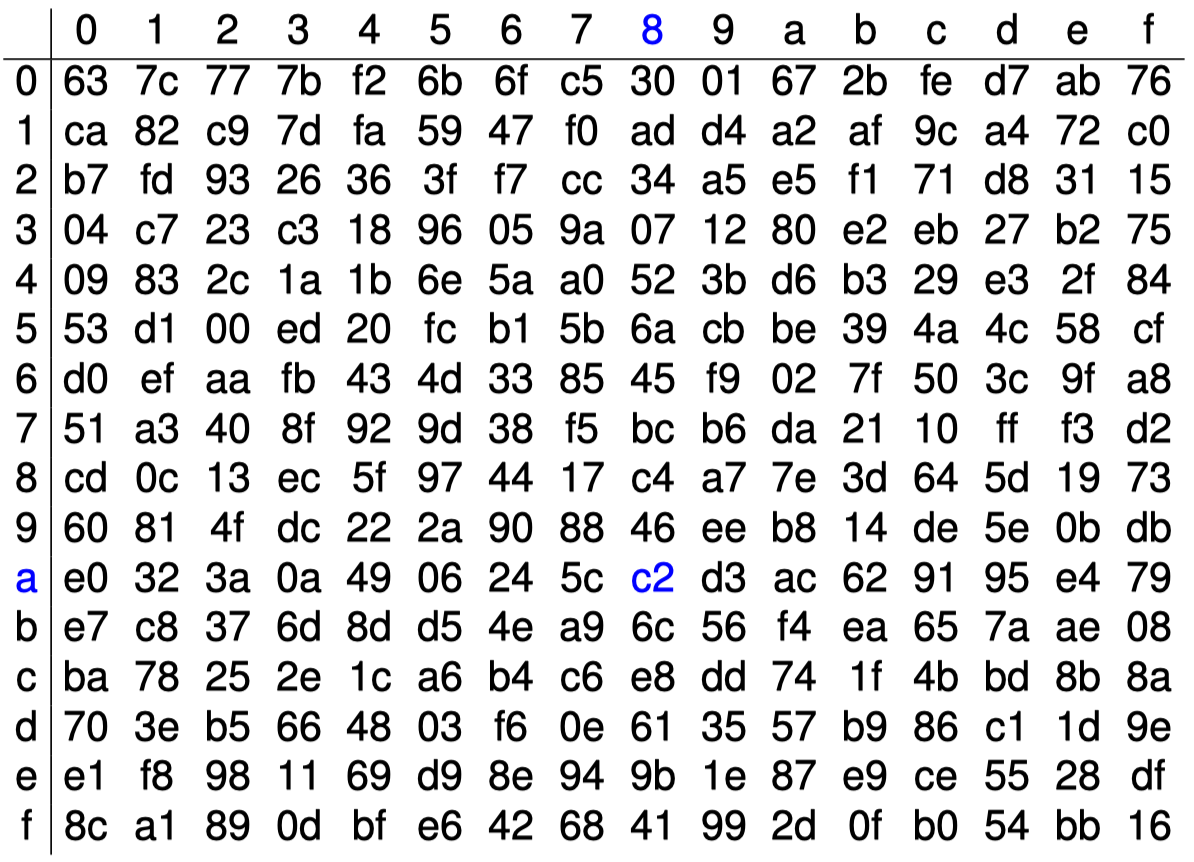
\includegraphics[width=\textwidth]{AES_S_Box.png}
		\caption{AES SBox}
	\end{figure}
\end{center}

Here is how Mix Columns is calculated: \begin{enumerate}
\item Read column $i$ of Sta\textbf{}te as a polynomial: $$(a_{0,i}, a_{1,i} , a_{2,i} , a_{3,i}) = a_{0,i} + a_{1,i} x + a_{2,i} x^2 + a_{3,i} x^3$$ Essentially, we interpret the coefficients as elements of the finite field $GF(2^8)$.
\item Multiply this polynomial with the constant polynomial $c(x) = \texttt{03} \cdot x^3 + \texttt{01} \cdot x^2 + \texttt{01} \cdot x + \texttt{02}$ and reduce modulo $x^4 - 1$. This gives a new polynomial: $b_{0,i} + b_{1,i} x + b_{2,i} x^2 + b_{3,i} x^3$
\end{enumerate}
Equivalently, \begin{algorithm}
Let $a(x) = a_0+a_1x+a_2x^2+a_3x^3$, where each $a_i \in GF(2^8)$\\
Let $c(x) = \texttt{03} \cdot x^3 + \texttt{01} \cdot x^2 + \texttt{01} \cdot x + \texttt{02}$ where \texttt{01, 02, 03} are elements in $GF(2^8)$ (written in hexadecimal)\\
To compute $a(x) \otimes c(x)$: \\
\hskip2.0em Compute $d(x) = a(x) \times c(x)$ (polynomial multiplication, where coefficient arithmetic is in $GF(2^8)$).\\
\hskip2.0em Divide by $x^4-1$ to find the remainder polynomial $r(x)$ (equivalently, replace $x^4$ by $1$, $x^5$ by $x$, and $x^6$ by $x^2$).
\hskip2.0em Then $a(x) \otimes c(x) = r(x)$.
\caption{The $\otimes c(x)$ Operation of AES}
\end{algorithm}


Finally, we get to encrypt using AES: 
\begin{algorithm}
	From the key $k$ derive $h + 1$ subkeys $k_0 , k_1 , ..., k_h$.\\
	$State \leftarrow $ plaintext\\
	$State \leftarrow State \oplus k_0$\\
	\For(){$i = 1...h-1$}{
		$State \leftarrow \texttt{SubBytes}(State)$ \\
		$State \leftarrow \texttt{ShiftRows}(State)$ \\
		$State \leftarrow \texttt{MixColumns}(State)$ \\
		$State \leftarrow State \oplus k_i$
	} 
	$State \leftarrow \texttt{SubBytes}(State)$ \\
	$State \leftarrow \texttt{ShiftRows}(State)$ \\
	$State \leftarrow State \oplus k_h$\\
	ciphertext $\leftarrow State$
	\caption{AES Encryption}
\end{algorithm}

\begin{algorithm}
	\caption{AES Decryption}
	From the key $k$ derive $h + 1$ subkeys $k_0 , k_1 , ..., k_h$.\\
	$State \leftarrow $ ciphertext\\
	$State \leftarrow State \oplus k_h$\\
	$State \leftarrow \texttt{InvShiftRows}(State)$ \\
	$State \leftarrow \texttt{InvSubBytes}(State)$ \\
	\For(){$i = h-1...1$}{
		$State \leftarrow State \oplus k_i$\\
		$State \leftarrow \texttt{InvMixColumns}(State)$ \\
		$State \leftarrow \texttt{InvShiftRows}(State)$ \\
		$State \leftarrow \texttt{InvSubBytes}(State)$ \\
	} 
	$State \leftarrow State \oplus k_0$\\
	plaintext $\leftarrow State$
\end{algorithm}

Note that \texttt{InvMixcolumns} is multiplication by $d(x) = \texttt{0e} + \texttt{09}x + \texttt{0d}x^2 + \texttt{0b}x^3$ modulo $x^4 - 1$.

As for AES Key Schedule: \begin{itemize}
\item For 128-bit keys, AES has 10 rounds, so we need 11 subkeys.
\item The first subkey $k 0 = (r_0 , r_1 , r_2 , r_3)$ is the actual AES key.
\item The second subkey is $k_1 = (r_4 , r_5 , r_6 , r_7 )$.
\item The third subkey is $k 2 = (r_8 , r_9 , r_{10} , r_{11})$.
\item $\cdots$
\item The eleventh subkey is $k_{10} = (r_{40} , r_{41} , r_{42} , r_{43} )$.
\end{itemize}

The functions $f_i : \{0, 1\}^{32} \rightarrow \{0, 1\}^{32}$ are defined as follows: \begin{enumerate}
\item The input is divided into 4 bytes: $(a, b, c, d)$.
\item Left-rotate the bytes: $(b, c, d, a)$.
\item Apply the AES S-box to each byte: $(S(b), S(c), S(d), S(a))$.
\item XOR the leftmost byte with the constant $\ell_i$, and output the result: $$(S(b) \oplus \ell_i, S(c), S(d), S(a))$$
\end{enumerate}
The constants $\ell_i$ are defined as follows: 

\begin{center}
	\begin{tabular}{cc|cc|cc|cc|cc}
		$i$ & $\ell_i$      & $i$ & $\ell_i$      & $i$ & $\ell_i$      & $i$ & $\ell_i$      & $i$ & $\ell_i$      \\
		\hline
		1   & \texttt{0x01} & 2   & \texttt{0x02} & 3   & \texttt{0x04} & 4   & \texttt{0x08} & 5   & \texttt{0x10} \\
		6   & \texttt{0x20} & 7   & \texttt{0x40} & 8   & \texttt{0x80} & 9   & \texttt{0x1b} & 10  & \texttt{0x36} 
	\end{tabular}
\end{center}
\newpage
\begin{center}
	\begin{figure}[h!]
		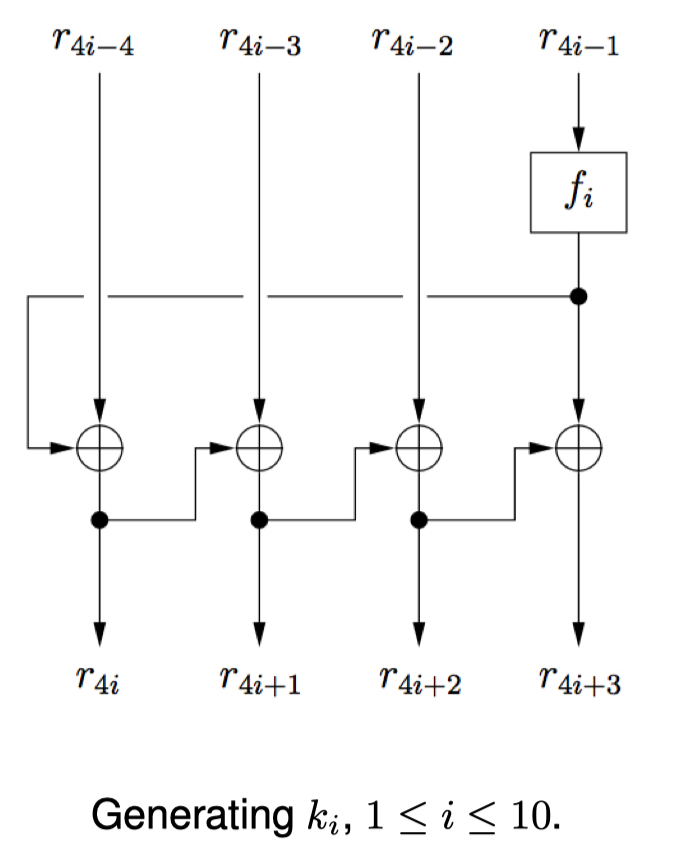
\includegraphics[width=0.5\textwidth]{AES_Key_Schedule.png}
		\caption{AES Key Schedule for 128-bit keys}
	\end{figure}
\end{center}

\subsection{Performance of SKES}

Speed benchmarks (2017) for software implementations on an Intel Core i9 2.9 GHz 6-core Coffee Lake (8950HK) using OpenSSL 1.1.1d.

\begin{center}
	\begin{tabular}{cccc}
		Algorithm      & block length (bits) & key length (bits) & speed (Mbytes/sec) \\
		\hline\hline
		RC4            & -                   & 128               & 644                \\
		ChaCha20       & -                   & 256               & 1846               \\
		DES            & 64                  & 56                & 98                 \\
		Triple-DES     & 64                  & 168               & 39                 \\
		AES (software) & 128                 & 128               & 254                \\
		AES (AES-NI)   & 128                 & 128               & 1632               
	\end{tabular}
\end{center}

\subsection{Block Cipher Modes of Operation}

How should we use a block cipher $E_k : \{0, 1\}^L \rightarrow \{0, 1\}^L$ to encrypt $m$?

We have: \begin{itemize}
\item Electronic Codebook (ECB) Mode: 
\begin{itemize}
	\item Encrypt blocks independently, one at a time: $c = c_1, c_2,..., c_t$ , where $c_i = E_k (m_i)$.
	\item Decryption: $m_i = E_k (c_i), i = 1, 2, ..., t$.
	\item Drawback: Identical plaintexts result in identical ciphertexts (under the same key), and thus ECB encryption is not (semantically) secure against chosen-plaintext attacks.
\end{itemize}
\begin{center}
	\begin{figure}[h!]
		\centering
		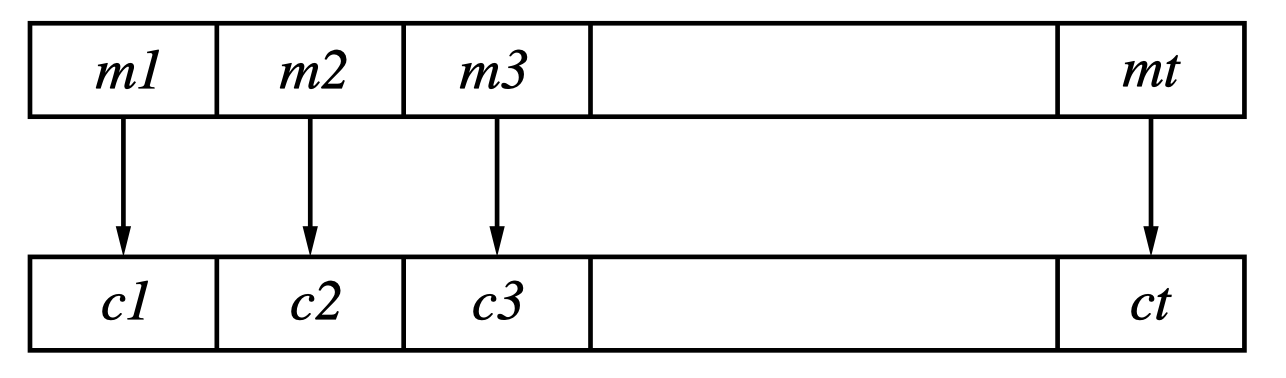
\includegraphics[width=\textwidth]{ECB.png}
		\caption{Electronic Codebook (ECB) Mode}
	\end{figure}
\end{center}
\item Cipher Block Chaining (CBC) Mode: 
\begin{itemize}
	\item Encryption: Select $c_0 \in_R \{0, 1\}^L$ ($c_0$ is a random non-secret IV). Then compute $c_i = E_k (m_i \oplus c_{i-1}), i = 1, 2, ...,t$.
	\item Ciphertext is $(c_0 , c_1 , c_2 , ..., c_t)$
	\item Decryption: $m_i = E_k (c_i) \oplus c_{i-1}, i = 1, 2,..., t$.
	\item Identical plaintexts with different IVs result in different ciphertexts and for this reason CBC encryption is (semantically) secure against chosen-plaintext attacks (for a well chosen block cipher $E$)
\end{itemize}
\end{itemize}
\begin{center}
	\begin{figure}[h!]
		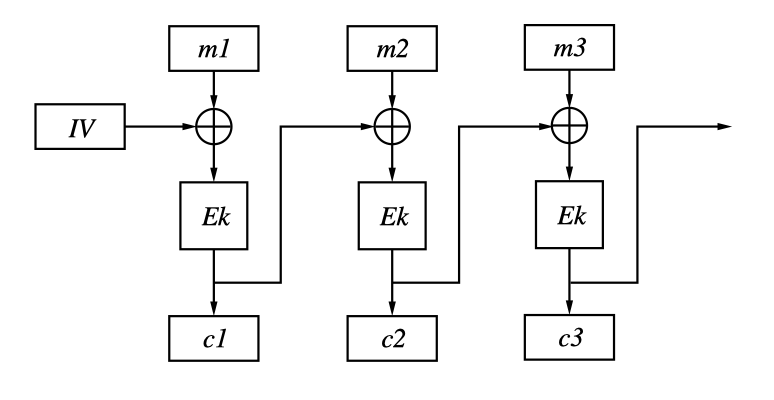
\includegraphics[width=0.5\textwidth]{CBC.png}
		\caption{Cipher Block Chaining (CBC) Mode}
	\end{figure}
\end{center}

% Section 3
\section{Hash Function}
\subsection{Definitions and Terminology}
\begin{definition}
	A \textbf{hash function} is a mapping $H$ such that:\begin{itemize}
	\item $H$ maps binary messages of arbitrary lengths $\leq L$ to outputs of a fixed length $n$:$$H: \{0, 1\}^{\leq L} \rightarrow \{0, 1\}^n$$
	($L$ is large, for example, $L = 2^{64}$; $n$ is small, for example $n = 256$)
	\item $H(x)$ can be efficiently computed for all $x \in \{0, 1\}^{\leq L}$
	\end{itemize}
\end{definition}
Notes: \begin{itemize}
\item $H$ is called an $n$-bit hash function.
\item $H(x)$ is called the \textbf{hash} or \textbf{message digest} of x.
\item The description of a hash function is public. There are no secret keys.
\item For simplicity, we will usually write $\{0, 1\}^*$ instead of $\{0, 1\}^{\leq L}$
\end{itemize}

\subsection{Hash Functions from Block Ciphers}
This one is called \textbf{Davies-Meyer hash function}. We let $E_k$ be an $m$-bit block cipher with $n$-bit key $k$, and let IV be a fixed $m$-bit initializing value.

\begin{algorithm}
	Break up $x\|1$ into $n$-bit blocks: $x = x_1, x_2 ,..., x_t$, padding out the last block with 0 bits if necessary.\\
	Define $H_0 = IV$\\
	\For(){$i = 1...t$}{
		Compute $H_i = E_{x_i} (H_{i-1}) \oplus H_{i-1}$
	}
	Define $H(x) = H_t$
	\caption{Davies-Meyer hash function}
\end{algorithm}

\begin{center}
	\begin{figure}[h!]
		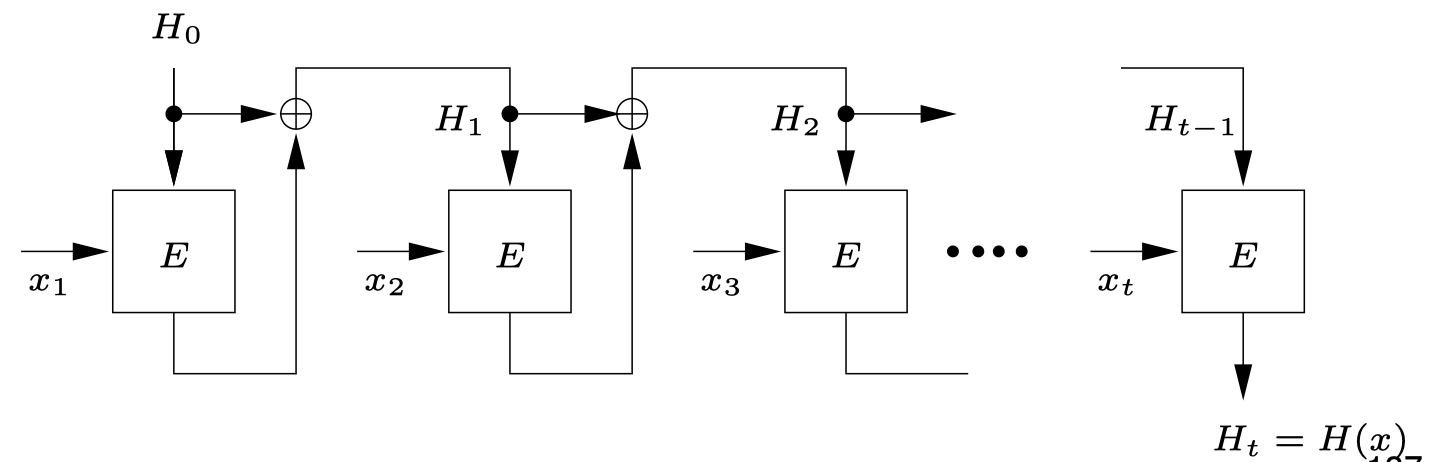
\includegraphics[width=\textwidth]{Davies_Meyer_Hash_Function.png}
		\caption{Davies Meyer Hash Function}
	\end{figure}
\end{center}
\newpage

\subsection{Preimage Resistance, 2nd Preimage Resistance, and Collision Resistance}
\begin{definition}
	\textbf{Preimage resistance}: Given a hash value $y \in_R \{0, 1\}^n$, it is computationally infeasible to find (with non-negligible probability of success) \textbf{any} $x \in \{0, 1\}^*$ such that $H(x) = y$. 
		
	$x$ is called a \textbf{preimage} of $y$
		
	$x \in_R S$ means that $x$ is chosen independently and uniformly at random from $S$.
\end{definition}

This could be useful in Password protection on a multi-user computer system: \begin{itemize}
\item Server stores $(userid, H(password))$ in a password file. Thus, if an attacker gets a copy of the password file, she does not learn any passwords.
\item Requires preimage-resistance
\end{itemize}

\begin{definition}
	\textbf{2nd preimage resistance}: Given an input $x \in_R \{0, 1\}^*$, it is computationally infeasible to find (with non-negligible probability of success) a second input $x' \in \{0, 1\}^*$, $x \neq x'$, such that $H(x') = H(x)$. 
\end{definition}
This could be useful in \textbf{Modification Detection Codes (MDCs)}:\begin{itemize}
\item To ensure that a message $m$ is not modified by unauthorized means, one computes $H(m)$ and protects $H(m)$ from unauthorized modification.
\item For example, virus protection.
\item Requires 2nd preimage resistance.
\end{itemize}

\begin{definition}
	\textbf{Collision resistance}: It is computationally infeasible to find (with non-negligible probability of success) two distinct inputs $x, x' \in \{0, 1\}^*$ such that $H(x) = H(x')$.
		
	The pair $(x, x')$ is called a collision for $H$.
\end{definition}

This could be useful in \textbf{Message digests for digital signature schemes}:\begin{itemize}
\item For reasons of efficiency, instead of signing a (long) message, the (much shorter) message digest is signed.
\item Requires preimage-resistance, 2nd preimage resistance, and collision resistance.
\item To see why collision resistance is required: Suppose that the legitimate signer Alice can find two messages $x_1$ and $x_2$ , with $x_1 \neq x_2$ and $H(x_1) = H(x_2)$.
\item Alice can sign $x_1$ and later claim to have signed $x_2$.
\end{itemize}

Relationship between PR, 2PR, and CR: \begin{itemize}
\item CR implies 2PR
\item 2PR does not guarantee CR
\item CR does not guarantee PR
\item if $H$ is ``somewhat'' random, i.e. all hash values have roughly the same number of preimages, then, CR implies PR
\item PR does not guarantee 2PR
\item 2PR implies PR (for somewhat uniform $H$)
\end{itemize}

\begin{proposition}
	Collision Resistance implies 2nd Preimage Resistance
\end{proposition}
\begin{proof}
	We prove the contrapositive. Suppose $H$ is not 2PR. 
	
	Let's select $x\in_R \{0,1\}^*$. Since $H$ is not 2PR, we can efficiently find $x' \in \{0,1\}^*$ with $x \neq x'$ and $H(x) = H(x')$. Thus, we have efficiently found a collision $(x, x')$ for $H$. Hence, $H$ is not CR. 
\end{proof}

\begin{proposition}
	2nd Preimage Resistance does not guarantee Collision Resistance
\end{proposition}
\begin{proof}
	Suppose that $H: \{0,1\}^* \rightarrow \{0,1\}^n$ is 2PR. Consider $\bar{H}: \{0,1\}^* \rightarrow \{0,1\}^n$ defined by: $$\bar{H}(x) = \begin{dcases}
	H(0) & \text{if } x = 1 (\text{This gives } \bar{H}(1) = H(0) = \bar{H}(0))\\
	H(x) & \text{if } x \neq 1
	\end{dcases}$$
	
	Suppose that $\bar{H}$ is not 2PR. So, given $x \in_R \{0,1\}^*$, we can efficiently find $x' \in \{0,1\}^*$, $x \neq x'$, with $\bar{H}(x') = \bar{H}(x)$. With probability essentially 1, we can assume that $x \neq 0, 1$. Hence, $\bar{H}(x) = H(x)$. Now, if $x' \neq 1$, then $\bar{H}(x') = H(x') = H(x)$; while if $x'=1$, then $\bar{H}(x') = \bar{H}(1) = H(0) = H(x)$. In either case, we have found a second preimage for $x$ with respect to $H$. So, $\bar{H}$ must be 2PR. 
	
	Also, $\bar{H}$ is not CR, since $(0,1)$ is a collision for $\bar{H}$
\end{proof}

\begin{proposition}
	Collision Resistance does not guarantee Preimage Resistance
\end{proposition}

\begin{proof}
	Suppose that $H: \{0,1\}^* \rightarrow \{0,1\}^n$ is CR. 
	
	Consider $\bar{H}: \{0,1\}^* \rightarrow \{0,1\}^{n+1}$ defined by $$\bar{H}(x) = \begin{dcases}
	1\|x & \text{if } x \in \{0,1\}^n\\
	0\|H(x) & \text{if } x \notin \{0,1\}^n
	\end{dcases}$$
	
	Then, $\bar{H}$ is CR (since $H$ is). And, $\bar{H}$ is not PR since preimages can be efficiently found for at least half of all $y \in \{0,1\}^{n+1}$
\end{proof}

\begin{proposition}
	if $H$ is ``somewhat'' random, i.e. all hash values have roughly the same number of preimages, then, Collision Resistance implies Preimage Resistance
\end{proposition}

\begin{proof}
	We prove the contrapositive. 
	
	Suppose $H$ is not PR. Select $x \in_R \{0,1\}^*$ and compute $y = H(x)$. Since $H$ is not PR, we can efficiently find a preimage $x'$ of $y$. 
		
	Since $H$ is somewhat uniform, we expect that $y$ has many preimages, and thus $x' \neq x$ with very high probability. Thus, $(x, x')$ is a collision for $H$ that we have efficiently found, so $H$ is not CR. 
\end{proof}

From now on, we shall assume that hash functions are somewhat uniform. 

\begin{proposition}
	Preimage Resistance does not guarantee 2nd Preimage Resistance
\end{proposition}

\begin{proof}
	Suppose $H: \{0,1\}^* \rightarrow \{0,1\}^n$ is PR.
	
	Define $\bar{H}: \{0,1\}^* \rightarrow \{0,1\}^n$ by $$\bar{H}(0, x_2, ..., x_t)$$
	
	Then, $\bar{H}$ is PR, but $\bar{H}$ is 2PR. 
\end{proof}

\begin{proposition}
	For ``somehwhat''uniform H. 2nd Preimage Resistance implies Preimage Resistance
\end{proposition}

We may refer to the following figure as a summary. 

\begin{center}
	\begin{figure}[h!]
		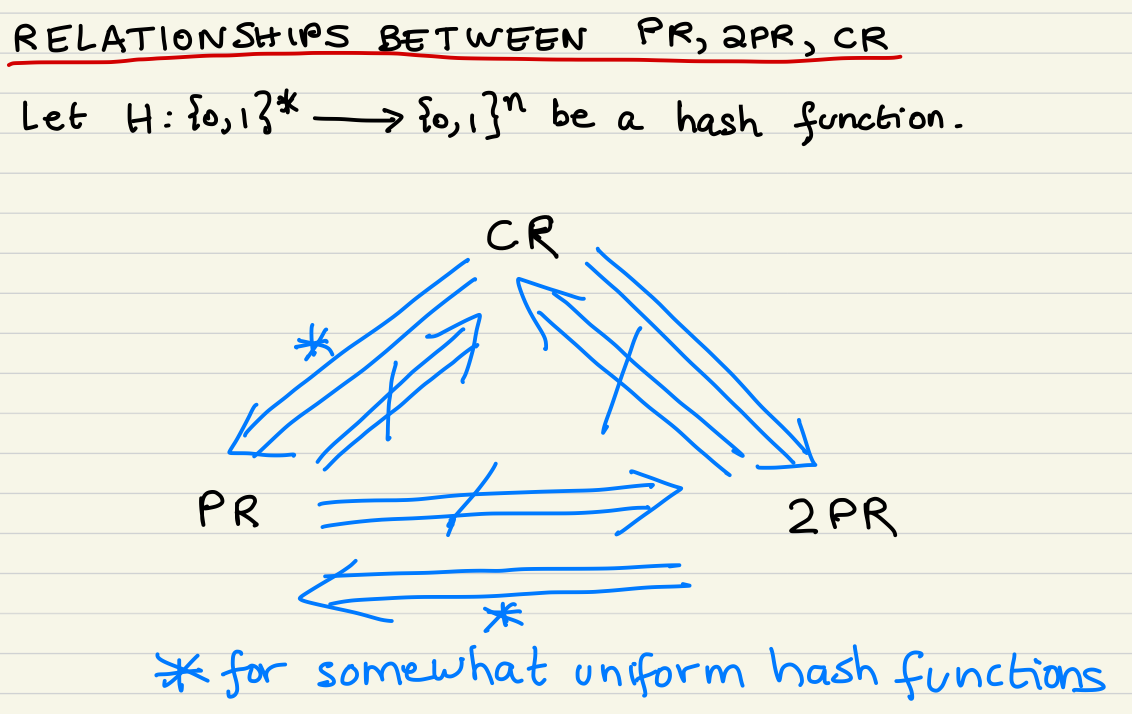
\includegraphics[width=\textwidth]{PR_2PR_CR.png}
		\caption{Relationship between PR, 2PR, and CR}
	\end{figure}
\end{center}
\subsection{Generic Attack}
\begin{definition}
	A \textbf{generic} attack on a hash function $H: \{0, 1\}^* \rightarrow \{0, 1\}^n$ does not exploit any properties the specific hash function may have.
\end{definition}

In the \textbf{analysis} of a generic attack, we view $H$ as a \textbf{random function} in the sense that for each $x \in \{0,1\}^*$, we assume that the value $y = H(x)$ was chosen by selecting $y \in_R {0, 1}^n$.

From a security point of view, a random function is an \textbf{ideal} hash function. However, random functions are not suitable for practical applications because they cannot be compactly stored.

\begin{algorithm}[H]
	Given $y \in_R \{0, 1\}^n$, repeatedly select arbitrary $x \in \{0, 1\}^*$ until $H(x) = y$
	\caption{Generic Attack for Finding Preimages}
\end{algorithm}
\begin{itemize}
	\item Expected number of steps is $\approx 2^n$
	\item This attack is infeasible if $n \geq 128$
	\item It has been proven that this generic attack for finding preimages is optimal, i.e., no faster generic attack exists
\end{itemize}
\begin{algorithm}[H]
	Select arbitrary $x \in \{0, 1\}^*$ and store $(H(x), x)$ in a table sorted by first entry. Continue until a collision is found.
	\caption{Generic Attack for Finding Collisions}
\end{algorithm}
\begin{itemize}
	\item Expected number of steps is $\sqrt{\pi2^n / 2} \approx \sqrt{2^n}$ (by birthday paradox)
	\item This attack is infeasible if $n \geq 256$.
	\item It has been proven that this generic attack for finding collisions is optimal in terms of the number of hash function evaluations
	\item Expected number of space required is $\sqrt{\pi2^n / 2} \approx \sqrt{2^n}$
\end{itemize}
\subsection{Van Oorschot and Wiener Parallel Collision Search}
\begin{itemize}
	\item Expected number of steps: $\sqrt{2^n}$
	\item Expected space required: negligible.
	\item Easy to parallelize: $m$-fold speedup with $m$ processors.
	\item Conclusion: If collision resistance is desired, then use an $n$-bit hash function with $n \geq 256$
\end{itemize}

We want to find a collision for $H: \{0,1\}^* \rightarrow \{0,1\}^n$, assuming that $H$ is a random function. 

In terms of notation, let $N = 2^n$. Let's define a sequence $\{x_i\}_{i \geq 0}$ by $x_0 \in_R \{0, 1\}^n$, and $x_i = H(x_{i-1})$ for $i \geq 1$. 

Let $j$ be the smallest index from which $x_j = x_i$ for some $i < j$; such $j$ must exist. Then $x_{j+\ell} = x_{i+\ell}$ for all $\ell \geq 1$. By the birthday paradox, $E[j] \approx \sqrt{\frac{\pi N}{2}} \approx \sqrt{N}$. In fact, $E[i] \approx \frac{1}{2}\sqrt{N}$ and $E[j-i] \approx \frac{1}{2}\sqrt{N}$. 

Now, $i \neq 0$ with overwhelming probability, in that event, $(x_{i-1}, x_{j-1})$ is a collision for $H$. 

\begin{center}
	\begin{figure}[h!]
		\centering
		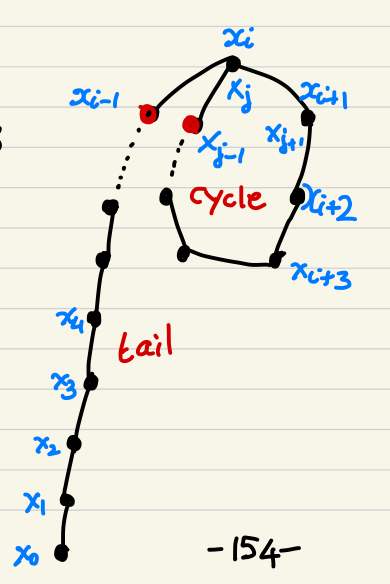
\includegraphics[width=0.2\textwidth]{VW_1.png}
		\caption{Main Idea of VW Search}
	\end{figure}
\end{center}

However, storage would be a problem (too many points to store). VW's idea is to store only \textbf{distinguished points}.

We can select an easily testable distinguishing property for elements of $\{0,1\}^n$ (for example, leading 32 bits are all 0). Let $\Theta$ be the proportion of elements of $\{0,1\}^n$ that are distinguished. 

In VW's algorithm, we compute $x_0, x_1, x_2, ...$ and only store the points in the sequence that are distinguished. 

\begin{center}
	\begin{figure}[h!]
		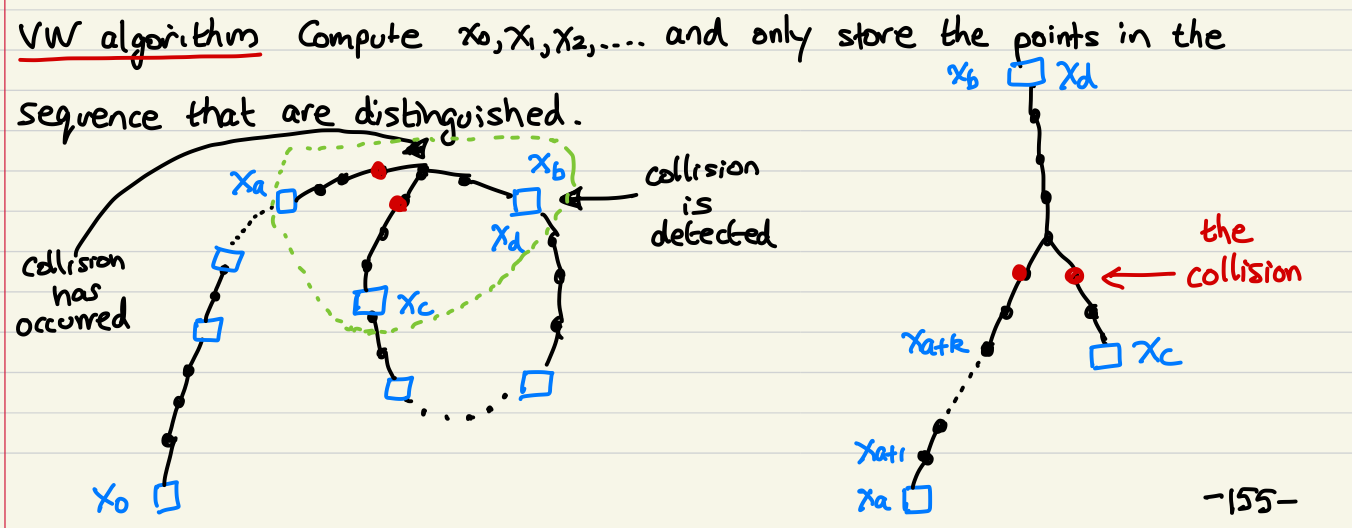
\includegraphics[width=\textwidth]{VW_2.png}
		\caption{VW's Search Flow}
	\end{figure}
\end{center}

\begin{algorithm}
	\textcolor{blue}{Stage 1: (Detecting a collision)}\\
	Select $x_0 \in_R \{0,1\}^n$\\
	Store $(x_0, 0, -)$ in a sorted table\\
	$LP \leftarrow x_0$ (LP means last point stored)\\
	\For(){$d=1,2,...$}{
		Compute $x_d = H(x_{d-1})$\\
		\If(){$x_d$ is distinguished}{
			\If(){$x_d$ is already in table, Say $x_d = x_b$ where $b < d$}{
				Go to Stage 2
			} 
			Store $(x_d, d, LP)$ in table\\
			$LP \leftarrow x_d$
		}
	}
	\textcolor{blue}{Stage 2: (Finding a collision)}\\
	Set $\ell_1 \leftarrow b-a$, $\ell_2 \leftarrow d-c$\\
	Suppose $\ell_1 \geq \ell_2$, set $k \leftarrow \ell_1 - \ell_2$\\
	Compute $x_{a+1}, x_{a+2}, ..., x_{a+R}$\\
	\For(){$m = 1,2,3...$}{
		Compute $(x_{a+k+m}, x_{c+m})$
	}
	Until $x_{a+k+m} = x_{c+m}$\\
	The collision is $(x_{a+k+m-1}, x_{c+m-1})$
	\caption{VW Collision Finding}
\end{algorithm}

The analysis of the algorithm is as follows: \begin{itemize}
\item Stage 1: the expected number of $H$-evalutations is $$\underbrace{\sqrt{\frac{\pi N}{2}}}_{\text{collision occurs}} + \underbrace{\frac{1}{\Theta}}_{\text{collision is detected}} \approx \sqrt{N} + \frac{1}{\Theta}$$
\item Stage 2: the expected number of $H$-evalutations is $\leq \frac{3}{\Theta}$
\item Overall the expected running time is $\sqrt{N} + \frac{4}{\Theta}$
\item Storage: $\approx \Theta\sqrt{N}(3n)$ (since each table entry has bit length $3n$)
\item For example, let $n = 128$. Take $\Theta = 1/2^{32}$. Then, the expected runtime of VW collision search is $2^{64}$ $H$-evaluations, which is feasible, and the expected storage is $241$ Gbytes. 
\end{itemize}

We can parallelized this algorithm by running a copy of VW on each of the $m$ processors. Report distinguished points to a central server. 

\begin{center}
	\begin{figure}[h!]
		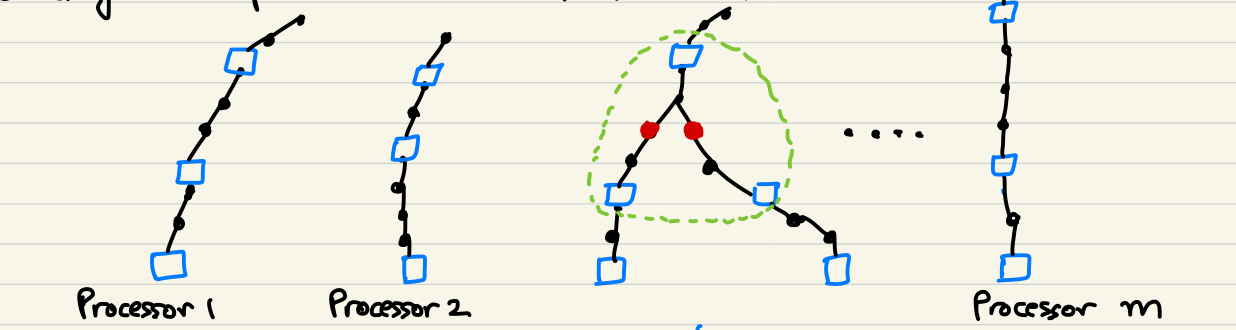
\includegraphics[width=\textwidth]{VW_3.png}
		\caption{Parallelizing VW Search}
	\end{figure}
\end{center}

The expected runtime would be $\sqrt{N} / m + \frac{4}{\Theta}$. The expected storage is $\Theta \sqrt{N}(3n)$ bits. 

This gives us a factor $m$ speedup. There are no communication between processors, and there are only occasional communication with central server. 


\subsection{Iterated Hash Function}
For iterated hash functions, we have: \begin{itemize}
\item Fixed \textbf{initializing value} $IV \in \{0,1\}^n$.
\item A \textbf{compression function} $f: \{0,1\}^{n+r} \rightarrow \{0,1\}^n$, which is efficiently computable. 
\end{itemize}

\begin{algorithm}
	\KwIn{$x$ has bitlength $b < 2^r$}
	\KwOut{$H(x)$}
	Break up $x$ into $r$-bit blocks $\bar{x} = x_1, x_2, ..., x_t$, padding out the last block with 0 bits if necessary.\\
	Define $x_{t+1}$, the \textbf{length block}, to hold the right-justified binary representation of $b$\\
	Define $H_0 = IV$
	\For(){$i=1,2,...,t+1$}{
		Compute $H_i = f(H_{i-1}, x_i)$
	}
	Output $H(x) = H_{t+1}$
	\caption{Iterated Hash Function}
\end{algorithm}

The $H_i$'s are called chaining variables. 

\begin{center}
	\begin{figure}[h!]
		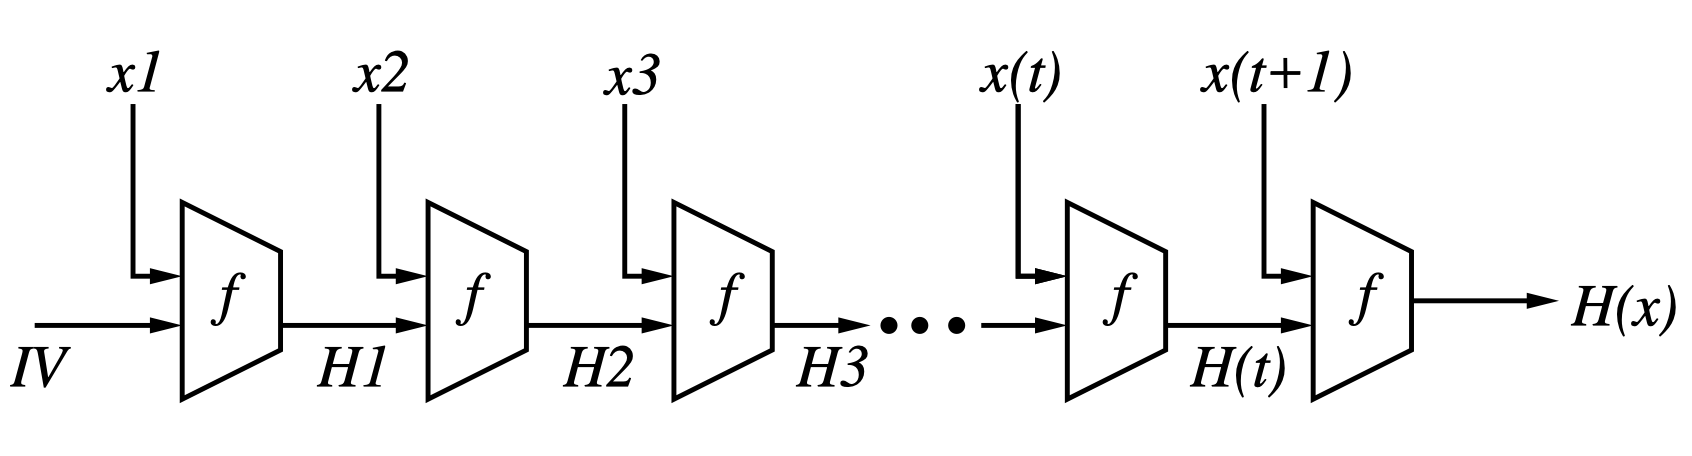
\includegraphics[width=\textwidth]{Iterated_Hash_Functions.png}
		\caption{Iterated Hash Functions}
	\end{figure}
\end{center}

\begin{theorem}
	\textbf{Merkle's Theorem}: If the compression function $f$ is collision resistant, then the hash function $H$ is also collision resistant. 
\end{theorem}
\begin{proof}
	Suppose that $H$ is not collision resistance, then we can efficiently find $x, x' \in \{0,1\}^*$ with $x \neq x'$, $H(x) = H(x')$. Let $\bar{x} = x_1,x_2, ..., x_t$ where $b = bitlength(x)$, $x_{t+1} = $ length block, and $\bar{x'} = x_1',x_2', ..., x_t'$ where $b' = bitlength(x')$, $x_{t+1}' = $ length block. 
	
	We can efficiently compute 
	\begin{center}
		\begin{tabular}{l|l}
			$H_0 = IV$                      & $H_0 = IV$                            \\
			$H_1 = f(H_0, x_1)$             & $H_1' = f(H_0, x_1')$                 \\
			$H_2 = f(H_1, x_2)$             & $H_2' = f(H_1', x_2')$                \\
			\vdots                          & \vdots                                \\
			$H_{t-1} = f(H_{t-2}, x_{t-1})$ & $H_{t'-1}' = f(H_{t'-2}', x_{t'-1}')$ \\
			$H_{t} = f(H_{t-1}, x_{t})$     & $H_{t'}' = f(H_{t'-1}', x_{t'}')$     \\
			$H_{t+1} = f(H_{t}, x_{t+1})$   & $H_{t'+1}' = f(H_{t'}', x_{t'+1}')$   \\
		\end{tabular}
	\end{center}
	Since $H(x) = H(x')$, we have $H_{t+1} = H_{t'+1}'$
	
	Now, if $b \neq b'$, then $x_{t+1} \neq x_{t'+1}'$. Then, $(H_t, x_{t+1}), (H_{t'}', x_{t'+1}')$ is a collision for $f$ that we have efficiently found. Hence, $f$ is not collision resistant. 
	
	Suppose that $b = b'$. Then $t = t'$ and $x_{t+1} = x_{t'+1}'$. Let $i$ be the largest index, $0 \leq i \leq t$ for which $$(H_i, x_{i+1}) \neq (H_i', x_{i+1}')$$
	Such an $i$ must exist, since $x \neq x'$. Then, $$H_{i+1} = f(H_i, x_{i+1}) = f(H_i', x_{i+1}') = H_{i+1}'$$
	So $(H_i, x_{i+1}), (H_{i}', x_{i+1}')$ is a collision for $f$ that we have efficiently found. Hence $f$ is not collision resistant. 
\end{proof}


Merkle’s theorem reduces the problem of designing collision-resistant hash functions to that of designing collision-resistant compression functions.

\subsection{Provable Security}
\begin{itemize}
	\item A major theme of cryptographic research is to formulate precise security definitions and assumptions, and then prove that a cryptographic protocol is \textbf{secure}.
	\item A \textbf{proof of security} is certainly desirable since it rules out the possibility of attacks being discovered in the future.
	\item However, it isn’t always easy to assess the practical security assurances (if any) that a security proof provides: \begin{itemize}
	\item The assumptions might be unrealistic, or false, or circular.
	\item The security proof might be fallacious.
	\item The security model might not account for certain kinds of realistic attacks.
	\item The security proof might be asymptotic.
	\item The security proof might have a large tightness gap.
\end{itemize}
\end{itemize}

\subsection{MDx-Family of Hash Functions}
\begin{itemize}
	\item \textbf{MDx} is a family of iterated hash functions.
	\item \textbf{MD4} was proposed by Ron Rivest in 1990.
	\item MD4 has \textbf{128-bit outputs}.
	\item Wang et al. (2004) found collisions for MD4 \textbf{by hand}.
	\item Leurent (2008) discovered an algorithm for finding MD4 preimages in $2^{102}$ steps.
\end{itemize}

MD5 Hash Function: \begin{itemize}
\item MD5 is a strengthened version of MD4.
\item Designed by Ron Rivest in 1991.
\item MD5 has 128-bit outputs.
\item Wang and Yu (2004) found MD5 collisions in $2^{39}$ steps.
\item MD5 collisions can now be found in $2^{24}$ steps (in a few seconds on a laptop computer).
\item Sasaki \& Aoki (2009) discovered a method for finding preimages for MD5 in $2^{123.4}$ steps.
\item So, MD5 should not be used if collision resistance is required, but is probably okay as a preimage-resistant hash func- tion.
\end{itemize}

\subsection{SHA-Family of Hash Functions}
SHA-1: \begin{itemize}
\item Secure Hash Algorithm (\textbf{SHA}) was designed by NSA and published by NIST in 1993 (FIPS 180).
\item \textbf{160-bit} iterated hash function, based on MD4.
\item Slightly modified to \textbf{SHA-1} (FIPS 180-1) in 1994 in order to fix an (undisclosed) security weakness.
\item Wang et al. (2005) discovered a collision-finding algorithm for SHA-1 that takes $2^{63}$ steps.
\item No preimage or 2nd preimage attacks (that are faster than the generic attacks) are known for SHA-1
\end{itemize}

SHA-2 Family: \begin{itemize}
\item In 2001, NSA proposed variable output-length versions of SHA-1.
\item Output lengths are \textbf{224} bits (SHA-224 and SHA-512/224), \textbf{256} bits (SHA-256 and SHA-512/256), \textbf{384} bits (SHA-384) and \textbf{512} bits (SHA-512).
\item As of 2020: No weaknesses in any of these hash functions have been found.
\item The security levels of these hash functions against collision-finding attacks is the same as the security levels of Triple-DES, AES-128, AES-192 and AES-256 against exhaustive key search attacks.
\item The SHA-2 hash functions are standardized in FIPS 180-2.
\end{itemize}

SHA-256: \begin{itemize}
\item It is an iterated hash function (Merkle meta-method).
\item $n = 256, r = 512$
\item Compression function is $f : \{0, 1\}^{256+512} \rightarrow \{0, 1\}^{256}$.
\item Input: bitstring $x$ of arbitrary bitlength $b \geq 0$
\item Output: $256$-bit hash value $H(x)$ of $x$.
\end{itemize}


Here is a table for SHA-256 Notation: \begin{center}
\begin{tabular}{ll}
	$A,B,C,D,E,F,G,H$     & 32 bits words                                                                       \\
	$+$                   & addition modulo $2^{32}$                                                            \\
	$\bar{A}$             & bitwise complement                                                                  \\
	$A \gg s$             & shift $A$ right through $s$ positions                                               \\
	$A \hookrightarrow s$ & rotate $A$ right through $s$ positions                                              \\
	$AB$                  & bitwise AND                                                                         \\
	$A \oplus B$          & bitwise exclusive-OR                                                                \\
	$f(A,B,C)$            & $AB \oplus \bar{A}C$                                                                \\
	$g(A,B,C)$            & $AB \oplus AC \oplus BC$                                                            \\
	$r_1(A)$              & $(A \hookrightarrow 2) \oplus (A \hookrightarrow 13) \oplus (A \hookrightarrow 22)$ \\
	$r_2(A)$              & $(A \hookrightarrow 6) \oplus (A \hookrightarrow 11) \oplus (A \hookrightarrow 25)$ \\
	$r_3(A)$              & $(A \hookrightarrow 7) \oplus (A \hookrightarrow 18) \oplus (A \gg 3)$              \\
	$r_4(A)$              & $(A \hookrightarrow 17) \oplus (A \hookrightarrow 19) \oplus (A \gg 10)$            \\
\end{tabular}
\end{center}

Here is a table for SHA-256 Constants: \begin{center}
\begin{tabular}{ll}
	$h_1 = $ \texttt{0x6a09e667} & $h_2 = $ \texttt{0xbb67ae85} \\
	$h_3 = $ \texttt{0x3c6ef372} & $h_4 = $ \texttt{0xa54ff53a} \\
	$h_5 = $ \texttt{0x510e527f} & $h_6 = $ \texttt{0x9b05688c} \\
	$h_7 = $ \texttt{0x1f83d9ab} & $h_8 = $ \texttt{0x5be0cd19} \\
\end{tabular}
\end{center}

These words were obtained by taking the first 32 bits of the fractional parts of the square roots of the first 8 prime numbers.

Here is a table for SHA-256 Per-round integer additive constants:
\begin{center}
	\begin{tabular}{ll}
		$y_0 = $ \texttt{0x428a2f98}    & $y_1 = $ \texttt{0x71374491}    \\
		$y_2 = $ \texttt{0xb5c0fbcf}    & $y_3 = $ \texttt{0xe9b5dba5}    \\
		\vdots                          & \vdots                          \\
		$y_{62} = $ \texttt{0xbef9a3f7} & $y_{63} = $ \texttt{0xc67178f2} \\
	\end{tabular}
\end{center}
These words were obtained by taking the first 32 bits of the fractional parts of the cube roots of the first 64 prime numbers.

SHA-256 Preprocessing: \begin{itemize}
\item Pad $x$ (with 1 followed by as few 0’s as possible) so that its bitlength is 64 less than a multiple of 512.
\item Append a 64-bit representation of $b \mod 2^{64}$.
\item The formatted input is $x_0, x_1, ..., x_{16m-1}$, where each $x_i$ is a 32-bit word.
\item Initialize chaining variables $$(H_1, H_2, ..., H_8) \leftarrow (h_1, h_2, ..., h_8)$$
\end{itemize}

SHA-256 Processing: \begin{itemize}
\item For each $i$ from $0$ to $m - 1$ do the following: 
\item Copy the $i$-th block of sixteen 32-bit words into temporary storage: $X_j \leftarrow x_{16i+j}$ , $0 \leq j \leq 15$.
\item Expand the 16-word block into a 64-word block: For $j$ from 16 to 63 do: $$X_j \leftarrow r_4 (X_{j-2}) + X_{j-7} + r_3 (X_{j-15}) + X_{j-16}$$
\item Initialize working variables:$$(A, B, C, ..., H) \leftarrow (H_1, H_2, ..., H_8)$$
\item For $j$ from 0 to 63 do:\begin{itemize}
\item $T_1 \leftarrow H + r_2(E) + f(E, F, G) + y_j + X$
\item $T_2 \leftarrow r_1(A) + g(A, B, C)$
\item $H \leftarrow G, G \leftarrow F, F \leftarrow E, E \leftarrow D + T_1$
\item $D \leftarrow C, C \leftarrow B, B \leftarrow A, A \leftarrow T_1 + T_2$
\end{itemize}
\item Update chaining values: $$(H_1, H_2, ..., H_8) \leftarrow (H_1+A, H_2+B, ..., H_8+H)$$
\end{itemize}

Then output SHA-256($x$) = $H_1\|H_2\|H_3\|H_4\|H_5\|H_6\|H_7\|H_8$

\subsection{Performance}
Speed benchmarks (2017) for software implementations on an Intel Core i9 2.9 GHz 6-core Coffee Lake (8950HK) using OpenSSL 1.1.1d.

\begin{center}
	\begin{tabular}{ccccc}
		Algorithm      & block length (bits) & key length (bits) & digest length (bits) & speed (Mbytes/sec) \\
		\hline\hline
		RC4            & -                   & 128               & -                    & 644                \\
		ChaCha20       & -                   & 256               & -                    & 1846               \\
		DES            & 64                  & 56                & -                    & 98                 \\
		Triple-DES     & 64                  & 168               & -                    & 39                 \\
		AES (software) & 128                 & 128               & -                    & 254                \\
		AES (AES-NI)   & 128                 & 128               & -                    & 1632               \\
		MD5            & 512                 & -                 & 128                  & 832                \\
		SHA-1          & 512                 & -                 & 160                  & 932                \\
		SHA-256        & 512                 & -                 & 256                  & 419                \\
		SHA-512        & 1024                & -                 & 512                  & 550                
	\end{tabular}
\end{center}

% section 4
\section{Message Authentication Code Schemes}
\begin{definition}
	A \textbf{message authentication code (MAC) scheme} is a family of functions $MAC_k : \{0, 1\}^* \rightarrow \{0,1\}^n$ parameterized by an $\ell$-bit key $k$, where each function $MAC_k$ can be efficiently computed.
	
	$t = MAC_k (x)$ is called the \textbf{MAC} or \textbf{tag} of $x$ with key $k$.
\end{definition}

\begin{center}
	\begin{figure}[h!]
		\centering
		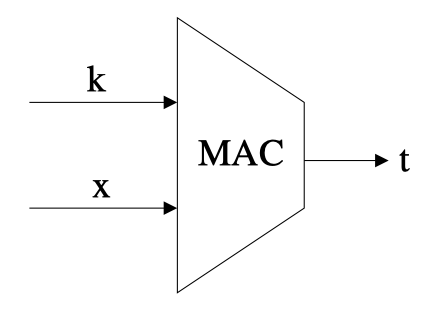
\includegraphics[width=0.4\textwidth]{MAC.png}
		\caption{Message Authentication Code (MAC)}
	\end{figure}
\end{center}

MAC schemes are used for providing (symmetric-key) \textbf{data integrity} and \textbf{data origin authentication}.

To provide data integrity and data origin authentication:\begin{enumerate}
\item Alice and Bob establish a secret key $k \in \{0,1\}^\ell$.
\item Alice computes tag $t=MAC_k (x)$ and sends $(x, t)$ to Bob.
\item Bob verifies that $t = MAC_k (x)$.
\end{enumerate}

Note that there is no confidentiality or non-repudiation. Also, to avoid replay, we should add a timestamp or sequence number.

\begin{center}
	\begin{figure}[h!]
		\centering
		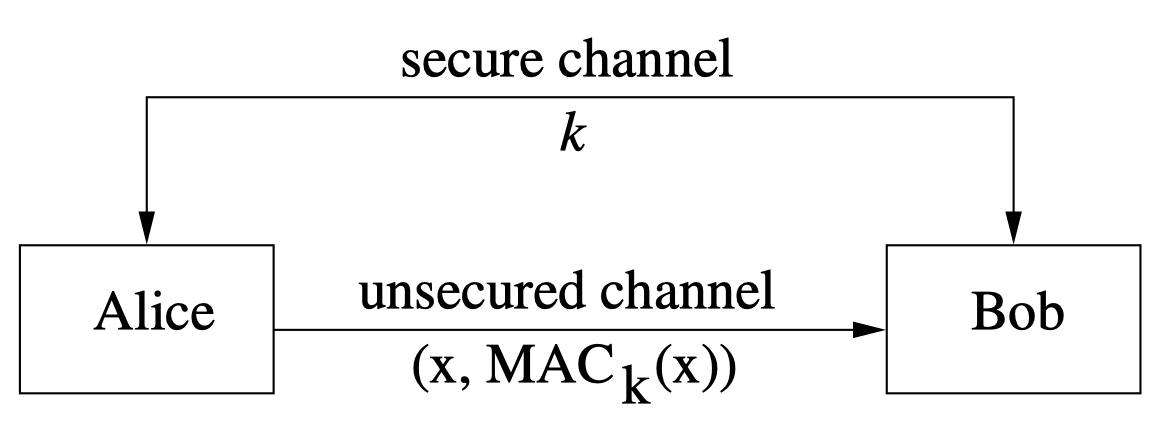
\includegraphics[width=\textwidth]{MAC_Application.png}
		\caption{Applications of MAC Schemes}
	\end{figure}
\end{center}

Let $k$ be the secret key shared by Alice and Bob.

The adversary does not know $k$, but is allowed to obtain (from Alice or Bob) tags for messages of her choosing. The adversary’s goal is to obtain the tag of \textbf{any} new message, i.e., a message whose tag she did not already obtain from Alice or Bob.


\begin{definition}
	A MAC scheme is \textbf{secure} if given some tags $MAC_k (x_i)$ for $x_i$'s of one’s own choosing, it is computationally infeasible to compute (with non-negligible probability of success) a message-tag pair $(x, MAC_k(x))$ for any new message $x$.
	
	More concisely, a MAC scheme is \textbf{secure} if it is \textbf{existentially unforgeable against chosen-message attack}
\end{definition}

An ideal MAC scheme has the following property:\begin{itemize}
\item For each key $k \in \{0,1\}^{\ell}$, the function $MAC_k : \{0, 1\}^{*} \rightarrow \{0, 1\}^{n}$ is a random function.
\item Ideal MAC schemes are useless in practice. However, when analyzing a generic attack on a MAC scheme, it is reasonable to assume that the MAC scheme is ideal.
\end{itemize}

\subsection{Generic Attacks on MAC schemes}
This attack is simple, we just guess the MAC of a message $x \in \{0,1\}^*$: \begin{algorithm}
Select $y \in_R \{0,1\}^n$ and guess that $MAC_k (x) = y$.
\caption{Generic Attack 1 on MAC schemes}
\end{algorithm}

If we assume that MAC k is a random function, the probability of success is $1/2^n$. Also, guesses cannot be directly checked. MAC guessing is infeasible if $n \geq 128$.


Also, we can perform exhaustive key search: \begin{algorithm}
Given $r$ known message-tag pairs $(x_1,t_1),..., (x_r,t_r)$, one can check whether a guess $k$ of the key is correct by verifying that $MAC_k (x_i) = t_i$, for $i=1, 2, ..., r$.
\caption{Generic Attack 2 on MAC schemes}
\end{algorithm}

Assuming that the $MAC_k$’s are random functions, the expected number of keys for which the tags verify is $1 + FK = 1 + (2^\ell -1)/2^{nr}$. The expected number of steps is $\approx 2^\ell$. Also, exhaustive search is infeasible if $\ell \geq 128$.

\subsection{MACs Based on Block Ciphers}
\begin{itemize}
	\item Let $E$ be an $n$-bit block cipher with key space $\{0,1\}^\ell$
	\item Assumption: Suppose that plaintext messages all have lengths that are multiplies of $n$.
	\item To compute $MAC_k (x)$: \begin{enumerate}
	\item Divide $x$ into $n$-bit blocks $x_1, x_2, ..., x_r$
	\item Compute $H_1 = E_k (x_1)$.
	\item For $2 \leq i \leq r$, compute $H_i = E_k (H_{i-1} \oplus x_i)$.
	\item Then $MAC_k (x) = H_r$.
	\end{enumerate}
\end{itemize}
\begin{center}
	\begin{figure}[h!]
		\centering
		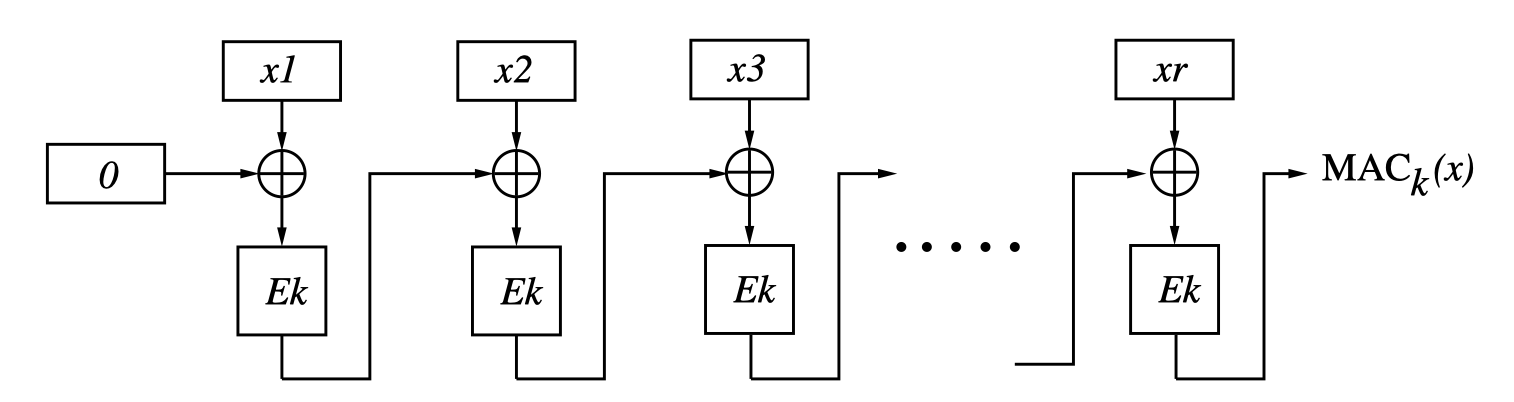
\includegraphics[width=\textwidth]{CBC_MAC.png}
		\caption{MACs Based on Block Ciphers}
	\end{figure}
\end{center}

\begin{theorem}
	Suppose that $E$ is an ``ideal'' encryption scheme. (That is, for each $k \in \{0, 1\}^\ell$, $E_k : \{0,1\}^n \rightarrow \{0, 1\}^n$ is a ``random'' permutation) Then $CBC-MAC$ with \textbf{fixed-length inputs} is a secure MAC scheme.
\end{theorem}

CBC-MAC (described above) is \textbf{not secure} if variable length messages are allowed.

Here is a chosen-message attack on CBC-MAC: \begin{enumerate}
\item Select an arbitrary $n$-bit block $x_1$.
\item Obtain the tag $t_1$ of the one-block message $x_1$ (so $t_1 = E_k (x_1)$).
\item Obtain the tag $t_2$ of the one-block message $t_1$ (so $t_2 = E_k (t_1)$).
\item Then $t_2$ is the tag of the 2-block message $(x_1 , 0)$ (since $t_2 = E_k (0 \oplus E_k (x_1)) = E_k(E_k (x_1)) = E_k (t_1)$).
\end{enumerate}

\subsubsection{Encrypted CBC-MAC (EMAC)}
One countermeasure for \textbf{variable-length} messages is \textbf{Encrypted CBC-MAC}: We encrypt the last block under a second key $s$: $EMAC_{k,s}(x) = E_s (H_r)$, where $H_r = CBC-MAC_k (x)$.

\begin{center}
	\begin{figure}[h!]
		\centering
		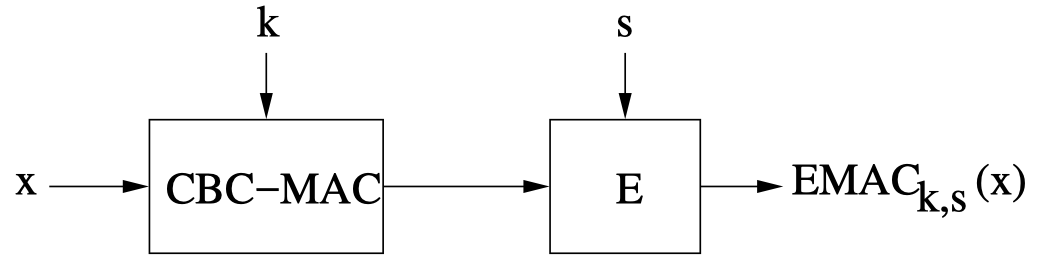
\includegraphics[width=\textwidth]{EMAC.png}
		\caption{Encrypted CBC-MAC (EMAC)}
	\end{figure}
\end{center}

\begin{theorem}
	Suppose that $E$ is an ``ideal'' encryption scheme. Then EMAC is a secure MAC scheme (for inputs of any length).
\end{theorem}

\subsection{MACs Based on Hash Functions}
Hash functions were not originally designed for message authentication; in particular they are not ``keyed'' primitives. 

How to use them to construct secure MACs?\begin{itemize}
\item Let $H$ be an iterated $n$-bit hash function (without the length-block).
\item Let $n + r$ be the input blocklength of the compression function $f : \{0, 1\}^{n+r} \rightarrow \{0, 1\}^n$.
\item Let $k\in \{0,1\}^n$
\item Let $K$ denote $k$ padded with $(r - n) 0$’s. (So $K$ has bitlength r)
\end{itemize}

We can consider Secret Prefix Method: we define $$MAC_k (x) = H(K, x)$$
\begin{center}
	\begin{figure}[h!]
		\centering
		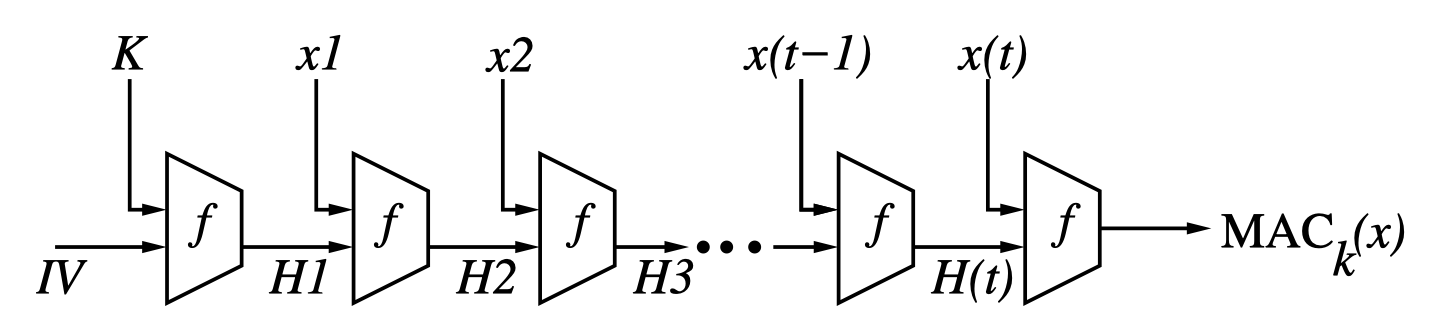
\includegraphics[width=\textwidth]{Secret_Prefix_Method.png}
		\caption{Secret Prefix Method}
	\end{figure}
\end{center}

This is \textbf{insecure}. Here is a \textbf{length extension attack}: \begin{enumerate}
\item Suppose that $(x, MAC_k (x))$ is known
\item Suppose that the bitlength of $x$ is a multiple of $r$.
\item Then $MAC_k (x \| y)$ can be computed for any $y$ (without knowledge of $k$).
\end{enumerate}
Also insecure if a length block is postpended to $K \| x$ prior to application of $H$.

Secret Suffix Method: we define $$MAC_k (x) = H(x, K)$$

\begin{center}
	\begin{figure}[h!]
		\centering
		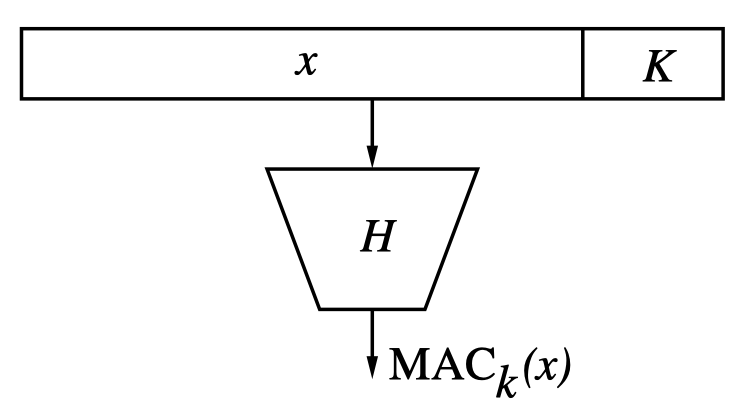
\includegraphics[width=0.7\textwidth]{Secret_Suffix_Method.png}
		\caption{Secret Suffix Method}
	\end{figure}
\end{center}

\begin{itemize}
	\item The attack on the secret prefix method does not work here.
	\item Suppose that a collision $(x_1 , x_2)$ can be found for $H$ (i.e., $H(x_1) = H(x_2)$). We assume that $x_1$ and $x_2$ both have bitlengths that are multiples of $r$. Thus $H(x_1, K) = H(x_2 , K)$, and so $MAC_k (x_1) = MAC_k (x_2)$. Then the MAC for $x_1$ can be requested, giving the MAC for $x_2$. Hence if $H$ is \textbf{not collision resistant}, then the secret suffix method MAC is \textbf{insecure}.
\end{itemize}

Envelope Method: we define $$MAC_k (x) = H(K, x, K)$$

\begin{center}
	\begin{figure}[h!]
		\centering
		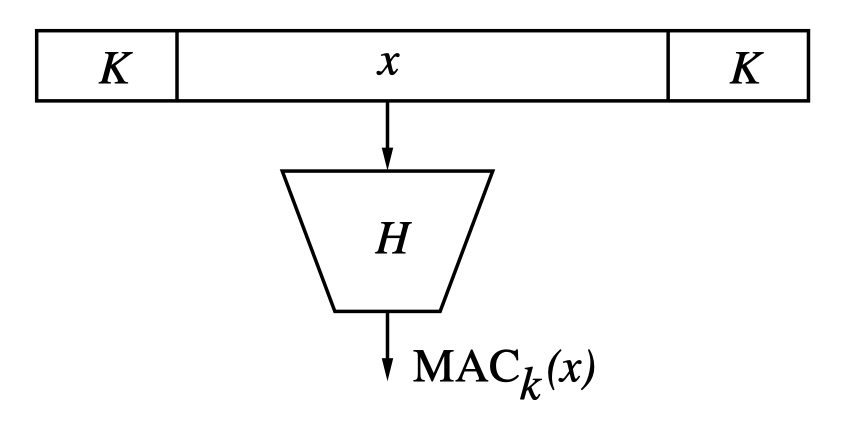
\includegraphics[width=0.7\textwidth]{Envelope_Method.png}
		\caption{Envelope Method}
	\end{figure}
\end{center}

\begin{itemize}
	\item The MAC key is used both at the start and end of the MAC computation.
	\item The envelope method appears to be secure (i.e., no serious attacks have been found).
\end{itemize}

$HMAC$: ``Hash-based'' MAC, developed by Bellare, Canetti and Krawczyk (1996).

We define two $r$-bit strings (in hexadecimal notation): ipad = \texttt{0x36}, opad = \texttt{0x5C}; each repeated $r/8$ times. Then, we define $$HMAC_k (x) = H(K \oplus opad, H(K \oplus ipad, x))$$

\begin{center}
	\begin{figure}[h!]
		\centering
		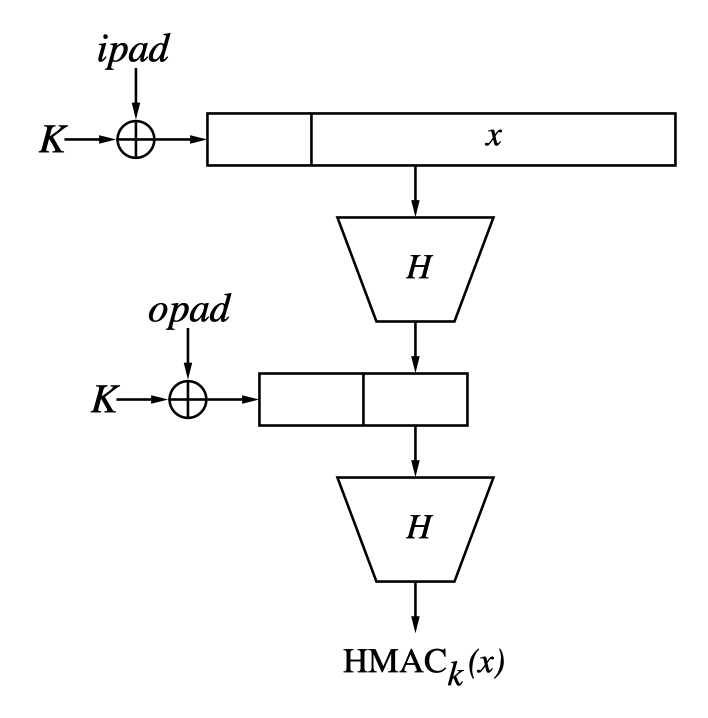
\includegraphics[width=0.7\textwidth]{HMAC.png}
		\caption{``Hash-based'' MAC}
	\end{figure}
\end{center}

\begin{theorem}
	Suppose that the compression function $f$ used in $H$ is a secure MAC with fixed length messages and a secret $IV$ as the key. Then HMAC is a secure MAC algorithm.
\end{theorem}

\subsection{Key Derivation Functions}
HMAC is commonly used as a \textbf{key derivation function} (KDF).
\begin{itemize}
	\item Suppose that Alice has a secret key $k$, and wishes to derive several session keys (e.g., to encrypt data in different communication sessions).
	\item Alice computes $sk_1 = HMAC_k (1), sk_2 = HMAC_k (2), sk_3 = HMAC_k(3), ...$.
	\item Without knowledge of $k$, an adversary is unable to learn anything about any particular session key $sk_j$ , even though it may have learnt some other session keys.
\end{itemize}
\subsection{GSM}
Global standards for mobile communications:\begin{itemize}
\item \textbf{2G, 2.5G}: GSM (Global System for Mobile Communication)
\item \textbf{3G}: UMTS (Universal Mobile Telecommunications System)
\item \textbf{4G}: LTE (Long Term Evolution)
\end{itemize}
GSM security is notable since it uses only symmetric-key primitives.

In terms of GSM security, we consider the following cryptographic ingredients:\begin{itemize}
\item \textbf{Enc}: A symmetric-key encryption scheme.
\item \textbf{MAC}: A symmetric-key MAC scheme.
\item \textbf{KDF}: A key derivation function.
\end{itemize}
Setup: \begin{itemize}
\item A SIM card manufacturer randomly selects a secret key $k$, and installs it in a SIM card. A copy of $k$ is given to the cell phone service provider.
\item When a user purchases cell phone service, she gets the SIM card which she installs in her phone.
\item A different key $k$ is chosen for each user.
\end{itemize}

Objectives:\begin{itemize}
\item \textbf{Entity authentication}: Cell phone service provider needs to be assured that entities accessing its service are legitimate subscribers.
\item \textbf{Confidentiality}: Users need the assurance that their cell phone communications are private.
\end{itemize}

\begin{algorithm}
	\textbf{Alice}: cell phone user\\
	\textbf{Bob}: cell phone service provider\\
	Alice sends an authentication request to Bob\\
	Bob selects a \textbf{challenge} $r \in_R \{0,1\}^{128}$, and sends $r$ to Alice.\\
	Alice’s SIM card uses $k$ to compute the \textbf{response} $t = MAC_k (r)$. Alice sends $t$ to Bob.\\
	Bob retrieves Alice’s key $k$ from its database, and verifies that $t = MAC_k (r)$.\\
	Alice and Bob compute an \textbf{encryption key} $K_E = KDF (r)$, and thereafter use the encryption algorithm $Enc_{K_E}$ to encrypt and decrypt messages for each other for the remainder of the session.
	\caption{How GSM Works}
\end{algorithm}

One drawback with using only symmetric-key crypto is that the SIM card manufacturer and the cell phone service providers have to securely maintain a large database of SIM keys $k$.

\section{Authenticaed Encryption}
\begin{itemize}
	\item A symmetric-key encryption scheme $E$ provides \textbf{confidentiality}, e.g., $E = AES$.
	\item A MAC scheme provides \textbf{authentication} (\textbf{data origin authentication} and \textbf{data integrity}), e.g., $MAC = HMAC$.
	\item What if confidentiality and authentication are \textbf{both} required?
\end{itemize}

\subsection{Encrypt-and-MAC}
\begin{algorithm}
	Alice sends $(c, t) = (E_{k_1} (m), MAC_{k_2} (m))$ to Bob, where $m$ is the plaintext and $k_1, k_2$ are secret keys she shares with Bob.\\
	Bob decrypts $c$ to obtain $m = E_{k_1} (c)$ and then verifies that $t = MAC_{k_2} (m)$.
	\caption{Encrypt-and-MAC}
\end{algorithm}

However, this generic method might have some security vulnerabilities, since MAC might leak information about the plaintext. 

\subsection{Encrypt-then-MAC}
\begin{algorithm}
	Alice sends $(c, t) = (E_{k_1} (m), MAC_{k_2} (E_{k_1} (m)))$ to Bob, where $m$ is the plaintext and $k_1 , k_2$ are secret keys she shares with Bob.\\
	Bob first verifies that $t = MAC_{k_2} (c)$ and then decrypts $c$ to obtain $m = E_{k_1}^{-1} (c)$.
	\caption{Encrypt-then-MAC}
\end{algorithm}

This method has been deemed to be secure, provided of course that the encryption scheme E and the MAC scheme employed are secure.

\subsubsection{Special-Purpose AE Schemes}

Many specialized authenticated encryption schemes have been developed, the most popular of these being \textbf{Galois/Counter Mode (GCM)}.

These modes can be faster than generic Encrypt-then-MAC, and also allow for the authentication (but not encryption) of ``header'' data.

\begin{example}
	AES-GCM: \begin{itemize}
		\item Authenticated encryption scheme proposed by David McGrew and John Viega in 2004.
		\item Adopted as a NIST standard in 2007.
		\item Uses the \textbf{CTR} mode of encryption and a custom-designed MAC scheme.
	\end{itemize}
\end{example}

\subsubsection{CTR: CounTeR Mode of Encryption}

Let $k \in_R \{0,1\}^{128}$ be the secret key. Let $M = (M_1, M_2 ,... , M_u)$ be a plaintext message, where each $M_i$ is a 128-bit block, $u \leq 2^{32} - 2$.

\begin{algorithm}
	To encrypt $M$, Alice does the following:\\
	Select $IV \in_R \{0, 1\}^{96}$\\
	Let $J_0 = IV \| 0^{31} \| 1$\\
	\For(){$i = 1$ to $u$}{
		$J_i \leftarrow J_{i-1} + 1$ [increment the counter]\\
		Compute $C_i = AES_k(J_i) \oplus M_i$
	}
	Send $(IV, C_1, ..., C_u)$ to Bob.
	\caption{CTR Encryption}
\end{algorithm}

\begin{algorithm}
	To decrypt, Bob does the following:\\
	Let $J_0 = IV \| 0^{31} \| 1$\\
	\For(){$i = 1$ to $u$}{
		$J_i \leftarrow J_{i-1} + 1$ [increment the counter]\\
		Compute $M_i = AES_k(J_i) \oplus C_i$
	}
	\caption{CTR Decryption}
\end{algorithm}

Note: \begin{itemize}
	\item CTR mode of encryption can be viewed as a stream cipher.
	\item As was the case with CBC encryption, identical plaintexts with different IVs result in different ciphertexts.
	\item It is critical that the IV \textbf{should not be repeated}; this can be difficult to achieve in practice.
	\item Unlike CBC encryption, CTR encryption is \textbf{parallelizable} (work with different counters).
	\item Note that $AES^{-1}$ is not used.
\end{itemize}

\subsubsection{Multiplying Blocks}
\begin{itemize}
	\item Let $a = a_0 a_1 a_2 ... a_{127}$ be a $128$-bit block.
	\item We associate the binary polynomial $a(x) = a_0 + a_1 x + a_2 x^2 + \cdots + a_{127} x^{127} \in \mathbb{Z}_2[x]$ with $a$.
	\item Let $f(x) = 1 + x + x^2 + x^7 + x^{128}$.
	\item If $a$ and $b$ are 128-bit blocks then define $c = a \bullet b$ to be the block corresponding to the polynomial $$c(x) = a(x) \cdot b(x) \mod f(x) \text{ in } \mathbb{Z}_2[x]$$\begin{itemize}
		\item That is, $c(x)$ is the remainder upon dividing $a(x) \cdot b(x)$ by $f(x)$, where coefficient arithmetic is performed modulo 2.
		\item This is multiplication in the \textbf{Galois Field} $GF(2^{128})$.
	\end{itemize}
\end{itemize}

\subsection{AES-GCM}
\begin{definition}
	Input of \textbf{AES-GCM}: \begin{itemize}
		\item Data to be authenticated (but not encrypted) $A = (A_1, A_2, ..., A_v)$
		\item Data to be encrypted and authenticated: $M = (M_1, M_2, ..., M_u)$
		\item Secret key $k \in_R \{0,1\}^{128}$
	\end{itemize}
	Output of \textbf{AES-GCM}: $(IV, A, C, t)$, where: \begin{itemize}
		\item $IV$ is a 96-bit initialization vector.
		\item $A = (A_1, A_2, ..., A_v)$ is the authenticated data.
		\item $C = (C_1 , C_2 , ..., C_u )$ is the encrypted/authenticated data.
		\item $t$ is a 128-bit authentication tag.
	\end{itemize}
\end{definition}

\begin{algorithm}
	Let $L = L_A \| L_M $, where $L_A, L_M$ are the bitlengths of $A$, $M$ expressed as 64-bit integers. ($L$ is the length block.)\\
	Select $IV \in_R \{0,1\}^{96}$ and let $J_0 = IV \| 0^{31} \| 1$\\
	\textcolor{blue}{// Encryption}\\
	\For(){$i = 1$ to $u$}{
		Compute $J_i = J_{i-1} + 1$\\
		Compute $C_i = AES_k (J_i) \oplus M_i$.
	}
	\textcolor{blue}{// Authentication}\\
	Let $T = 0^{128}$\\
	Compute $H = AES_k (0^{128})$\\
	\For(){$i = 1$ to $v$}{
		$T \leftarrow (T \oplus A_i) \bullet H$
	}
	\textcolor{blue}{// $T = ((((0 + A_1)H + A_2)H + A_3)H + \cdots + A_v)H = A_1H^v + A_2H^{v-1} + \cdots + A_{v-1}H^2 + A_vH$}\\
	\For(){$i = 1$ to $u$}{
		$T \leftarrow (T \oplus C_i) \bullet H$
	}
	$T \leftarrow (T \oplus L) \bullet H$\\
	\textcolor{blue}{// $T = A_1H^{u+v+1} + A_2H^{u+v} + \cdots + A_vH^{u+2} + C_1H^{u+1} + \cdots + C_uH^2 + LH$}\\
	\textcolor{blue}{// $T = f_{A, M}(H)$, $f_{A, M}(x) = A_1x^{u+v+1} + \cdots + A_vx^{u+2} + C_1x^{u+1} + \cdots + C_ux^2+Lx \in GF(2^{128})[x]$}\\
	Compute $t = AES_k (J_0) \oplus T$\\
	\textcolor{blue}{// Hence, $t = AES_k(J_0) \oplus f_{A, M}(H)$}\\
	Output: $(IV, A, C, t)$
	\caption{AES-GCM Encryption/Authentication}
\end{algorithm}

A secret key should be used to encrypt at most $2^{32}$ messages.
\newpage
Here is an example of AES-GCM encryption and authentication, where authentication data $A$ is one-block long ($v = 1$), and plaintext data $M$ is two-blocks long ($u = 2$).
\begin{center}
	\begin{figure}[h!]
		\centering
		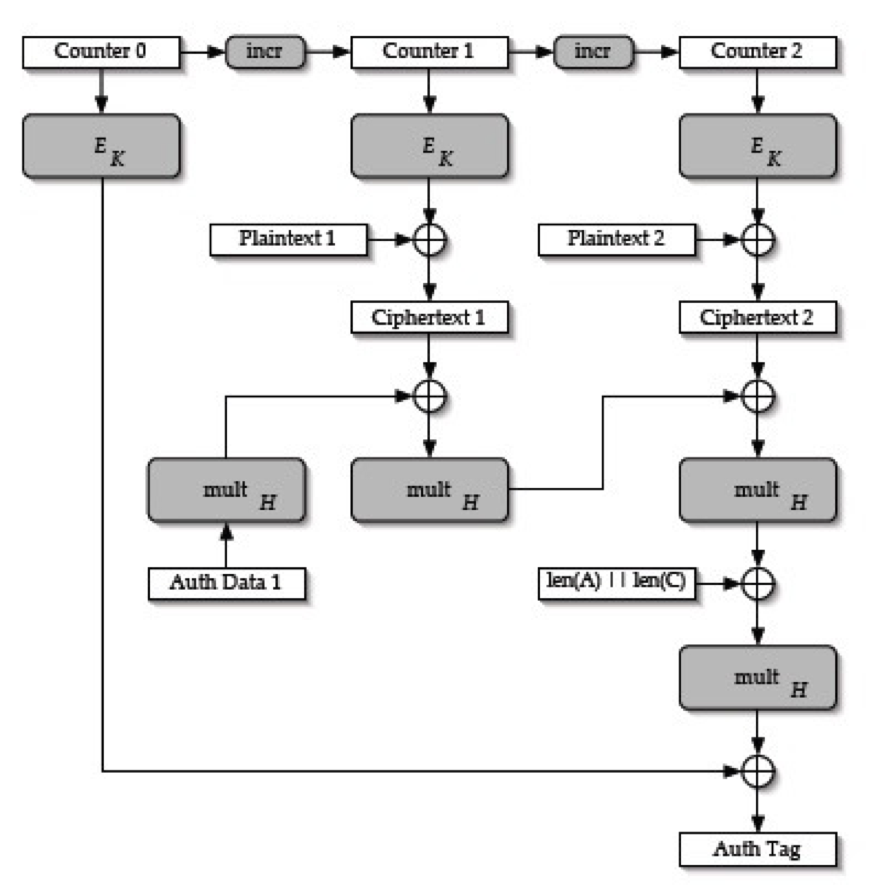
\includegraphics[width=0.8\textwidth]{AES_GCM.png}
		\caption{AES-GCM Encryption/Authentication}
	\end{figure}
\end{center}
\newpage
\begin{algorithm}
	Upon receiving $(IV, A, C, t)$, Bob does the following:\\
	Let L = $L_A \| L_C$ , where $L_A , L_C$ are the bitlengths of $A$, $C$ expressed as 64-bit integers.\\
	\textcolor{blue}{// Authentication}\\
	Let $T = 0^{128}$\\
	Compute $H = AES_k (0^{128})$\\
	\For(){$i = 1$ to $v$}{
		$T \leftarrow (T \oplus A_i) \bullet H$
	}
	\For(){$i = 1$ to $u$}{
		$T \leftarrow (T \oplus C_i) \bullet H$
	}
	$T \leftarrow (T \oplus L) \bullet H$\\
	Compute $t' = AES_k (J_0) \oplus T$\\
	\If(){$t' = t$}{
		proceed to decryption
	} \Else(){
		reject
	}
	\textcolor{blue}{// Decryption}\\
	Let $J_0 = IV \| 0^{31} \| 1$\\
	\For(){$i = 1$ to $u$}{
		Compute $J_i = J_{i-1} + 1$\\
		Compute $M_i = AES_k (J_i) \oplus C_i$
	}
	Accept and output $(A, M)$
	\caption{AES-GCM Decryption/Authentication}
\end{algorithm}


For AES-GCM, authentication only: \begin{itemize}
	\item Consider $AES_GCM$ with no $M$, so $u = 0$, $L_M = 0$
	\item The message to be authenticated is $A = (A_1, A_2, ..., A_v)$, where $v \leq \ell$. The tag is $(IV, t)$, where $IV \in_R \{0,1\}^{96}$ and $t = AES_k(J_0) + f_A(H)$, and $J_0 = IV\|0^{31}\|1$, $H = AES_k(0)$
	\item The attack goal is: Eve has message-tag pairs (for messages of her choosing): $(A^j, IV^j, t^j)$, $1 \leq j \leq r$. Her goal is to produce a message-tag forgery $(A^*, IV^*, t^*)$ where $A^* \notin \{A^1,A^2,..., A^r\}$
	\item We can assume that no two IV's in this list are the same
	\item We can also assume that Eve does not know $k$ or $H$
\end{itemize}

\begin{proposition}
	AES-GCM is secure if we consider authentication only. 
\end{proposition}
\begin{proof}
	Suppose that Eve outputs a forgery $(A^*, IV^*, t^*)$: \begin{itemize}
		\item If $IV^* \notin \{IV^1, IV^2, ..., IV^t\}$, then $J_0^* \notin \{J_0^1, ..., J_0^r\}$, and so Eve doesn't know $AES_k(J_0^*)$, which serves as a one-time pad for $f_{A^*}(H)$. Thus, the probability that Eve can output a valid tag (i.e. $t^* = AES_k(J_0^*) + f_{A^*}(H)$) is only $1/2^{128}$
		\item Suppose that $IV^* = IV^j$ for some $1 \leq j \leq r$, so $J_0^* = J_0^j$. Then, \begin{align*}
			t^*-t^j &= AES_k(J_0^*) + f_{A^*}(H) - AES_k(J_0^j) + f_{A^j}(H)\\
			&=f_{A^*}(H) - f_{A^j}(H)
		\end{align*}
		So, Eve has produced $A^*, A^j$, and $\alpha$ such that $\alpha = f_{A^*}(H) - f_{A^j}(H)$, without knowledge of $H$. But this can only be done with negligible probability, as the following lemma shows
	\end{itemize}
\end{proof}

\begin{lemma}
	For all distinct $A, B \in (\{0,1\}^{128})^{\leq \ell}$ and $\alpha \in \{0,1\}^{128}$, $Pr[f_A(H) - f_B(H) = \alpha]  \leq (\ell + 1) / 2^{128}$ (which is negligible), where the probability is assessed over random choices of $H \in \{0,1\}^{128}$
\end{lemma}

\begin{proof}
	Let $A, B \in (\{0,1\}^{128})^{\leq \ell}$ with $A \neq B$, and let $\alpha \in \{0,1\}^{128}$. 

	Suppose $A \in \{0,1\}^{128v}$, and $B \in \{0,1\}^{128w}$. Then, \begin{align*}
		f_A(H) - f_B(H) - \alpha &= (A_1H^{v+1} + A_2H^v + \cdots + A_vH^2 + L_AH)\\
		&-(B_1H^{w+1} + B_2H^w + \cdots + B_vH^2 + L_BH) - \alpha
	\end{align*}
	which is a polynomial in $H$ of degree $\leq \max(v,w) +1 \leq \ell + 1$.

	Since a non-zero polynomial of degree $\ell+1$ can have at most $\ell +1$ roots, there are at most $\ell + 1$ $H \in \{0,1\}^{128}$ satisfying $f_A(H) - f_B(H) - \alpha = 0$
\end{proof}

Here are some Features of AES-GCM: \begin{itemize}
	\item Performs authentication and encryption.
	\item Supports authentication only (by using empty $M$).
	\item Very fast implementations on Intel and AMD processors because of special \textbf{AES-NI} and \textbf{PCLMULQDQ} instructions for the AES and $\bullet$ operations.
	\item Encryption and decryption can be \textbf{parallelized}
	\item AES-GCM can be used in \textbf{streaming mode}
	\item Security is justified by a security proof: Original McGrew-Viega security proof (2004) was wrong. The proof was fixed in 2012 by Iwata-Ohashi-Minematsu.
	\item AES-GCM is widely used today.
\end{itemize}

\subsection{Encryption at Google}

\begin{center}
	\begin{figure}[h!]
		\centering
		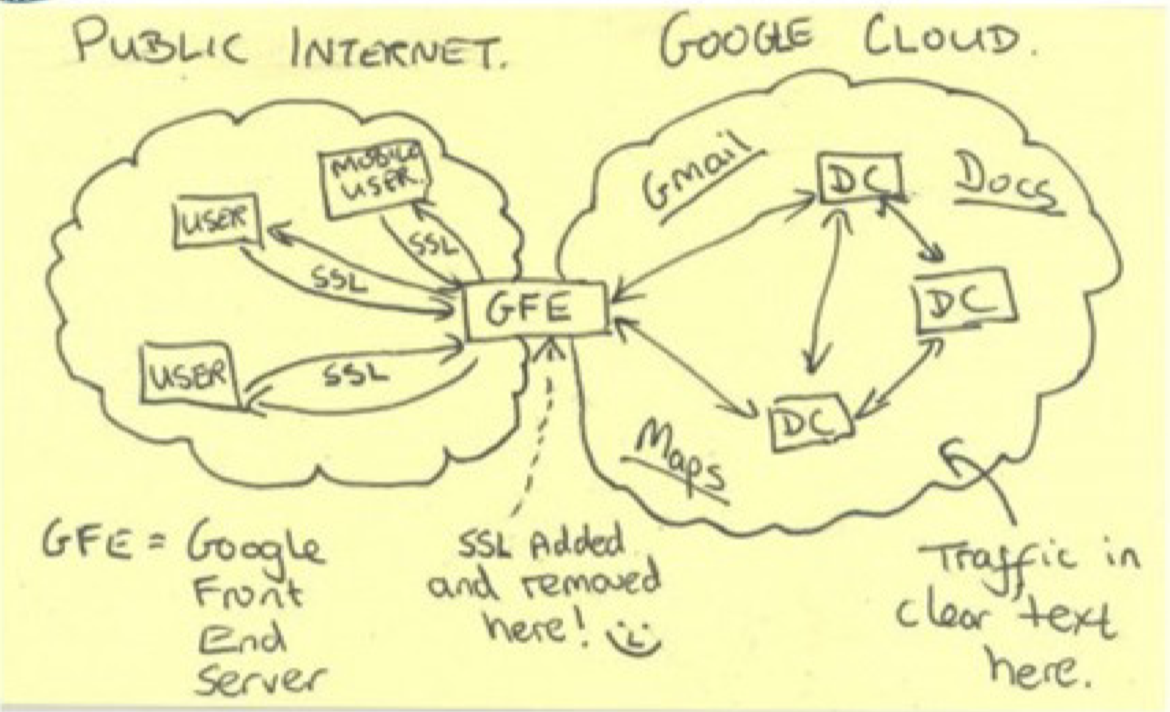
\includegraphics[width=\textwidth]{Google's_Encryption.png}
		\caption{Google's Encryption Flow}
	\end{figure}
\end{center}

Google has 21 data centres around the world: \begin{itemize}
	\item A data centre (DC) contains tens of thousands of servers.
	\item Lots of physical security (cameras, biometric identification, metal detectors, vehicle barriers, etc.)
	\item Communication between these servers and the outside world is all done via Google Front End (GFE) servers.
	\item Servers within a data centre communicate via a LAN (Local Area Network).
	\item Servers in different data centres communicate via a WLAN (Wide Local Area Network).
\end{itemize}

Google Data Security (Google wants to protect): \begin{enumerate}
	\item Data \textbf{communicated} between individual users (browsers) and Google (GFEs): \begin{itemize}
	\item Data is encrypted and authenticated using TLS.
	\item Symmetric-key enc. (e.g., AES), symmetric-key authentication (e.g., HMAC); authenticated enc. (e.g., AES-GCM); key establishment (e.g., RSA public-key enc., ECDH); public key certificates (RSA signatures).
	\item TLS is used by \textbf{all} web servers and browsers (not Google specific).
	\end{itemize}
	\item Data \textbf{communicated} between Google servers (perhaps in different data centres): \begin{itemize}
		\item Data is secured using Google’s version of TLS (Application Layer Transport Security, \textbf{ALTS})
		\item ALTS handles roughly $10^{10}$ remote procedure calls (RPCs) per second.
	\end{itemize}
	\item Data \textbf{stored} at data centres.
\end{enumerate}

\subsubsection{Key Management Service (KMS)}
\begin{itemize}
	\item All data stored within Google data centres is encrypted with \textbf{AES256-GCM} (GCM = Galois Counter Mode). AES128-CTR + HMAC-SHA256 (Encrypt-then-MAC) is used in some legacy applications.
	\item The KMS manages the many AES secret keys that are used to encrypt/decrypt data by the many storage services within data centres.
	\item Some of the KMS requirements:\begin{itemize}
		\item \textbf{Availability}: $> 99.9995\%$ requests are served.
		\item \textbf{Latency}: $99\%$ of requests are served in $< 10$ ms.
		\item \textbf{Scalability}: Handle $\approx 10^7$ requests/second.
		\item \textbf{Security}: Effortless and foolproof \textbf{key rotation}
		\item \textbf{Efficiency}: To minimize number of machines needed.
	\end{itemize}
\end{itemize}

Google’s Key Hierarchy: \begin{enumerate}
	\item \textbf{Storage systems} (millions of processes). Encrypts data with \textbf{DEKs} (Data Encryption Keys).
	\item \textbf{KMS} (tens of thousands). Encrypts DEKs with \textbf{KEKs} (Key Encryption Keys).
	\item \textbf{Root KMS} (hundreds). Encrypts KEKs with \textbf{KMS Master Keys}.
	\item \textbf{Root KMS Master Key Distributor} (hundreds). Encrypts KMS Master Keys with the Root KMS Master Key.
	\item \textbf{Physical safes} (two). The Root KMS Master Key is backed up on hardware devices.
\end{enumerate}

\subsubsection{Google's storage systems}

Suppose that a storage system wishes to encrypt some data item $m$. åThe storage system does the following: \begin{enumerate}
	\item Break up $m$ into \textbf{chunks}, $m_1, ..., m_\ell$. Each chunk can be up to several Gigabytes in size
	\item Generate $\ell$ \textbf{Data Encryption Keys} (DEKs), $k_1, ..., k_\ell$. Multiple sources of entropy are sampled (e.g., Intel’s RDRAND instruction; inter-packet arrival times; measurement of disk seeks). The samples are then combined and hashed using a key derivation function (KDF) to produce a 256-bit secret key.
	\item Encrypt with \textbf{AES256-GCM}: $c_1 = AES_{k_1} (m_1),...,c_\ell = AES_{k_\ell}(m_\ell)$.
	\item Send the DEKs $k_1, ..., k_\ell$ to a KMS.
	\item Receive the wrapped (encrypted) keys $w_1, ..., w_\ell$ from the KMS. The KMS encrypts the DEKs with its \textbf{Key Encryption Keys} (KEKs).
	\item Store $(c_1, w_1),..., (c_\ell, w_\ell)$ These encrypted chunks are replicated and distributed across Google’s storage systems.
\end{enumerate}

To decrypt a chunk $(c_j , w_j)$: \begin{enumerate}
	\item The storage system sends the wrapped key $w_j$ to the KMS.
	\item The KMS decrypts $w_j$ using the appropriate KEK, and sends the DEK $k_j$ to the storage system.
	\item The storage system decrypts $c_j$ using $k_j$.
\end{enumerate}

Notes: \begin{itemize}
	\item Each data chunk has a \textbf{unique identifier}.
	\item The KMS maintains an \textbf{Access Control List (ACL)} to ensure that a data chunk can only be decrypted by the authorized storage system.
	\item Note that each chunk of data is encrypted using a different DEK. This ensures that if a DEK is compromised, then only one chunk of data is potentially compromised.
	\item The storage system does not store the DEKs $k_1, ..., k_\ell$
	\item If a chunk of data $m_j$ is updated, it is re-encrypted with a new DEK $k_j'$ rather than using the old DEK $k_j$.
\end{itemize}

\subsubsection{Google's Key Management Services}
\begin{itemize}
	\item Key Management Services (KMSs) generate the AES256-GCM \textbf{Key Encryption Keys} (KEKs), and maintain the Access Control Lists (one ACL list for each KEK)
	\item The KMS encrypts/decrypts DEKs using the KEKs, in accordance with the ACL.
	\item The KEKs never leave the KMS.
	\item The KMS also maintains an audit trail of when a KEK was used
	\item KEKs are \textbf{rotated} (i.e., changed). The standard rotation frequency is once every 90 days.
\end{itemize}

\subsubsection{Google's Root KMS}
\begin{itemize}
	\item The \textbf{Root KMS} wraps KEKs with AES256-GCM \textbf{KMS Master Keys}. There are about a dozen KMS Master Keys. The Root KMSs are run on dedicated secured machines in Google’s data centres.
	\item The KMS Master Keys are wrapped with the AES256-GCM \textbf{Root KMS Master Key}. The Root KMS Master Key is stored in RAM on the Root KMS machines. \textbf{The Root KMS Master Key Distributor} ensures that all Root KMSs always have the same version of the Root KMS Master Key.
\end{itemize}

\subsubsection{Google's Physical Safes}
\begin{itemize}
	\item The Root KMS Master Key is backed up on two hardware devices stored in physical safes in highly secured areas in two physically separated Google locations.
	\item Fewer than 20 Google employees have access to these safes.
	\item The backups will be used if Google ever has to do a complete reboot.
\end{itemize}

\section{Introduction to Public-Key Cryptography}
\subsection{Drawbacks with Symmetric-Key Cryptography}
\subsubsection{Key Establishment Problem}

The shared secret keys can then be used to achieve confidentiality (e.g., using AES), or authentication (e.g., using HMAC), or both (e.g., using AES-GCM). However, How do Alice and Bob establish the secret key $k$?

Method 1: \textbf{Point-to-point key distribution}. (Alice selects the key and sends it to Bob over a secure channel) 

\begin{center}
	\begin{figure}[h!]
		\centering
		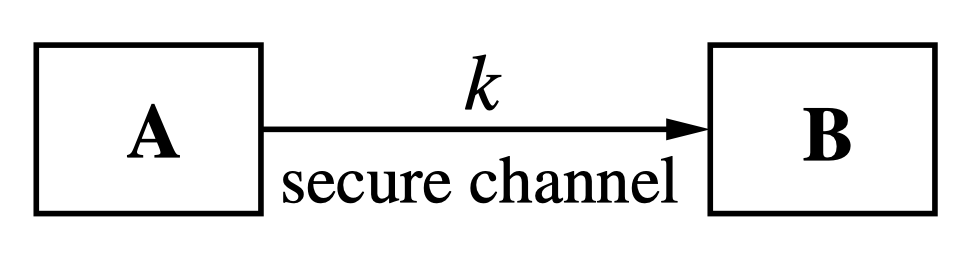
\includegraphics[width=0.5\textwidth]{Point_to_Point_Key_Distribution.png}
		\caption{Point to Point Key Distribution}
	\end{figure}
\end{center}

The secure channel could be: \begin{itemize}
	\item A trusted courier.
	\item A face-to-face meeting.
	\item Installation of an authentication key in a SIM card.
\end{itemize}
However, This is generally not practical for large-scale applications.

Method 2: Use a \textbf{Trusted Third Party (TTP) T}.
\begin{itemize}
	\item Each user $A$ shares a secret key $k_{AT}$ with $T$ for a symmetric-key encryption scheme $E$.
	\item To establish this key, $A$ must visit $T$ once.
	\item $T$ serves as a \textbf{key distribution centre} (KDC): \begin{enumerate}
		\item $A$ sends $T$ a request for a key to share with $B$.
		\item $T$ selects a session key $k$, and encrypts it for $A$ using $k_{AT}$.
		\item $T$ encrypts $k$ for $B$ using $k_{BT}$.
	\end{enumerate}
\end{itemize}

\begin{center}
	\begin{figure}[h!]
		\centering
		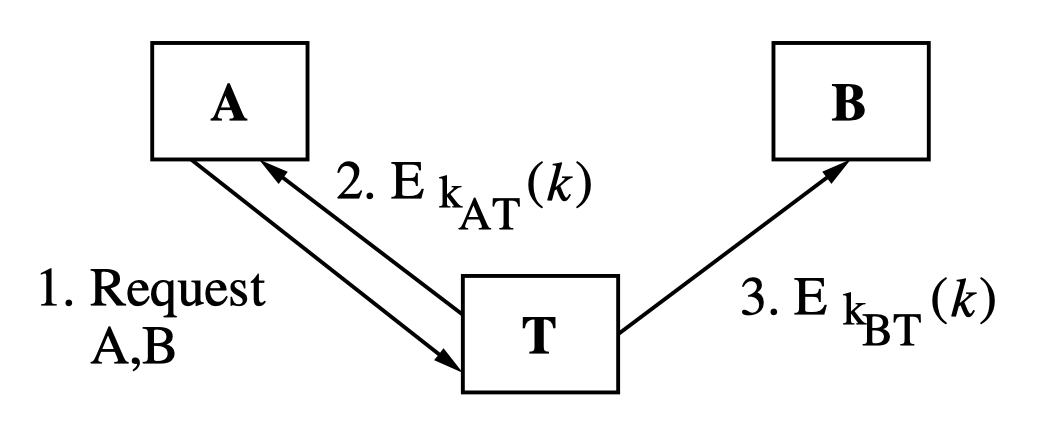
\includegraphics[width=0.7\textwidth]{Trusted_Third_Party.png}
		\caption{Relationship}
	\end{figure}
\end{center}

Drawbacks of using a KDC: \begin{enumerate}
	\item The TTP must be unconditionally trusted.
	\item The TTP is an attractive target.
	\item The TTP must be on-line.\begin{itemize}
		\item Potential bottleneck.
		\item Critical reliability point.
	\end{itemize}
\end{enumerate}

\subsubsection{Key Management Problem}
In a network of $n$ users, each user has to share a different key with every other user. Each user thus has to store $n - 1$ different secret keys. The total number of secret keys is ${n \choose 2} \approx n^2 /2$

\begin{center}
	\begin{figure}[h!]
		\centering
		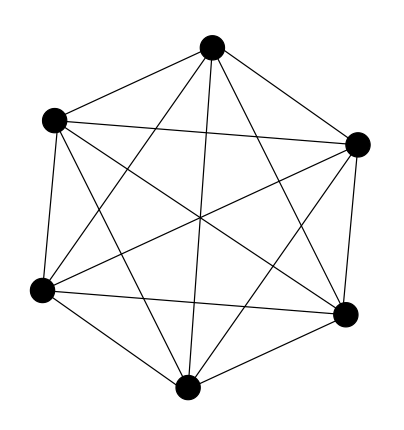
\includegraphics[width=0.5\textwidth]{Key_Management_Problem.png}
		\caption{Key Management Problem}
	\end{figure}
\end{center}

\subsubsection{Non-Repudiation is Impractical}
Strictly speaking, symmetric-key techniques cannot be used to achieve non-repudiation. This is because both Alice and Bob knows the secret keys. You will never know if Bob leaks the secret key to others or not. 
\subsection{Public-Key Cryptography}
The idea of Public-Key Cryptography is communicating parties a priori share some authenticated (but non-secret) information.
\begin{center}
	\begin{figure}[h!]
		\centering
		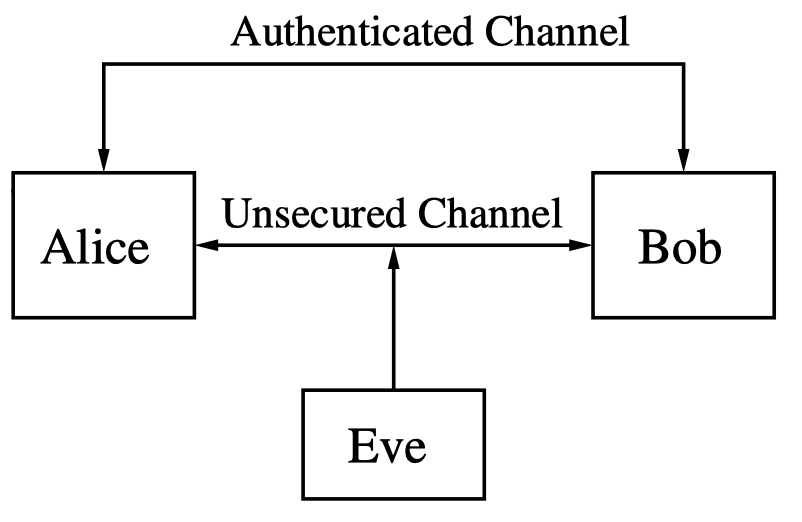
\includegraphics[width=0.7\textwidth]{Public_Key_Cryptography.png}
		\caption{Public Key Cryptography}
	\end{figure}
\end{center}

\subsubsection{Merkle Puzzles}
The goal is that Alice and Bob establish a secret session key by communicating over an authenticated (but non-secret) channel. Here is what to do: \begin{enumerate}
	\item Alice creates $N$ \textbf{puzzles} $P_i$ , $1 \leq i \leq N$ (e.g., $N = 10^9$). Each puzzle takes $t$ hours to solve (e.g., $t = 5$). The solution to $P_i$ reveals a 128-bit \textbf{session key} $sk_i$ and a randomly-selected 128-bit \textbf{serial number} $n_i$ (which Alice selected and stored).
	\item Alice sends $P_1, P_2, ..., P_N$ to Bob.
	\item Bob selects $j$ at random from $[1, N]$ and solves puzzle $P_j$ to obtain $sk_j$ and $n_j$.
	\item Bob sends $n_j$ to Alice.
	\item The secret session key is $sk_j$.
\end{enumerate}

An eavesdropper has to solve $500,000,000$ puzzles on average to determine the puzzle index $j$ (and thus $sk_j$).

\begin{example}
	We could make $P_i = AES-CBC_{k_i} (sk_i , n_i , n_i )$, where $k i = (r_i \| 0^{88})$ and $r_i$ is a randomly selected 40-bit string.

	$P_i$ can be solved in $2^{40}$ steps by exhaustive key search. But an eavesdropper has to do $\sim 500,000,000$ of this exhaustive key search, which is obviously infeasible. 
\end{example}

\begin{algorithm}
	Each entity $A$ does the following:\\
	Generate a key pair $(P_A , S_A)$.\\
	$S_A$ is $A$’s \textbf{secret key}.\\
	$P_A$ is $A$’s \textbf{public key}.
	\caption{Key Pair Generation for Public-Key Cryptography}
\end{algorithm}

\begin{itemize}
	\item \textbf{Security requirement}: It should be infeasible for an adversary to recover $S_A$ from $P_A$.
	\item For example, we can take $S_A = (p, q)$ where $p$ are $q$ are randomly-selected prime numbers; $P_A = p \cdot q$.
\end{itemize}

\begin{algorithm}
	To encrypt a secret message $m$ for Bob, Alice does:\\
	Obtain an \textbf{authentic} copy of Bob’s public key $P_B$ .\\
	Compute $c = E(P_B , m)$; $E$ is the encryption function.\\
	Send $c$ to Bob.
	\caption{Public-Key Encryption}
\end{algorithm}

\begin{algorithm}
	To decrypt $c$, Bob does:\\
	Compute $m = D(S_B , c)$; $D$ is the decryption function.
	\caption{Public-Key Decryption}
\end{algorithm}

\begin{center}
	\begin{figure}[h!]
		\centering
		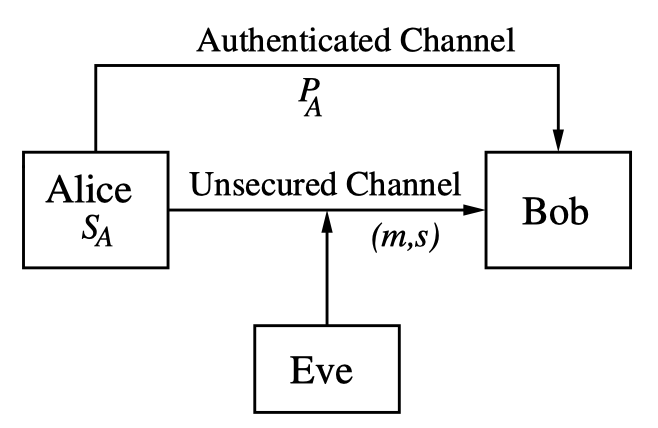
\includegraphics[width=0.5\textwidth]{Digital_Signatures.png}
		\caption{Digital Signatures}
	\end{figure}
\end{center}
\newpage
\begin{algorithm}
	To \textbf{sign} a message m, Alice does:\\
	Compute $s = Sign(S_A, m)$. \\
	Send $m$ and $s$ to Bob.
	\caption{Public-Key Digital Signatures}
\end{algorithm}

\begin{algorithm}
	To \textbf{verify} Alice’s signature $s$ on $m$, Bob does:\\
	Obtain an \textbf{authentic} copy of Alice’s public key $P_A$.\\
	Accept if $Verify(P_A , m, s)$ = ``Accept''.
	\caption{Public-Key Digital Verification}
\end{algorithm}

Suppose that Alice generates a signed message $(m, s)$, then \textbf{anyone} who has an authentic copy of Alice’s public key $P_A$ can verify the authenticity of the signed message. 

This authentication property cannot be achieved with a symmetric-key MAC scheme. Hence, digital signatures are widely used to \textbf{sign software updates} which are then broadcast to computers around the world.

\subsubsection{Public-Key Versus Symmetric-Key}
Advantages of public-key cryptography: \begin{itemize}
	\item No requirement for a secured channel.
	\item Each user has only 1 key pair, which simplifies key management.
	\item A signed message can be verified by anyone.
	\item Facilitates the provision of non-repudiation services (with digital signatures).
\end{itemize}

Disadvantages of public-key cryptography:\begin{itemize}
	\item Public-key schemes are slower than their symmetric-key counterparts.
\end{itemize}

\subsubsection{Hybrid Schemes}

\begin{algorithm}
	To \textbf{encrypt a secret signed message} $m$, Alice does:\\
	Compute $s = Sign(S_A , m)$.\\
	Select a secret key $k$ for a symmetric-key encryption scheme such as AES.\\
	Obtain an authentic copy of Bob’s public key $P_B$.\\
	Send $c_1 = E(P_B , k)$ and $c_2 = AES_k (m, s)$.
	\caption{Hybrid Scheme Encryption}
\end{algorithm}

\begin{algorithm}
	To recover $m$ and verify its authenticity, Bob does:\\
	Decrypt $c_1 : k = D(S_B , c_1)$.\\
	Decrypt $c_2$ using $k$ to obtain $(m, s)$.\\
	Obtain an authentic copy of Alice’s public key $P_A$.\\
	Check that $Verify(P_A , m, s)$ = ``Accept''.
	\caption{Hybrid Scheme Decryption}
\end{algorithm}

\subsection{Algorithmic Number Theory}
\subsubsection{Fundamental Theorem of Arithmetic}
\begin{theorem}
	\textbf{Fundamental Theorem of Arithmetic}: Every integer $n \geq 2$ has a unique prime factorization (up to ordering of factors).
\end{theorem}
Interesting questions:\begin{itemize}
	\item Given an integer $n \geq 2$, how do we find its prime factorization \textbf{efficiently}?
	\item How do we \textbf{efficiently} verify an alleged prime factorization of an integer $n \geq 2$?
	\item Given an integer $n \geq 2$, how do we \textbf{efficiently} decide whether $n$ is prime or composite?
\end{itemize}
\subsubsection{Basic Concepts from Complexity Theory}
\begin{definition}
	An \textbf{algorithm} is a ``well-defined computational procedure'' (e.g., a Turing machine) that takes a variable input and eventually halts with some output.

	For an integer factorization algorithm, the \textbf{input} is a positive integer n, and the \textbf{output} is the prime factorization of $n$.
\end{definition}
\begin{definition}
	The \textbf{efficiency} of an algorithm is measured by the scarce resources it consumes (e.g. time, space, number of processors, number of chosen plaintext-ciphertext pairs).
\end{definition}

\begin{definition}
	The \textbf{input size} is the number of bits required to write down the input using a reasonable encoding.

	The size of a positive integer $n$ is $\floor{\log_2 n}{} + 1$ bits. Note that $k = \log_2 n \Leftrightarrow n = 2^k$
\end{definition}

\begin{definition}
	The \textbf{running time} of an algorithm is an upper bound as a function of the input size, of the worst case number of basic steps the algorithm takes over all inputs of a fixed size.
\end{definition}

\begin{definition}
	An algorithm is a \textbf{polynomial-time} (efficient) algorithm if its (expected) running time is $O(k^c)$, where $c$ is a fixed positive integer, and $k$ is the \textbf{input size}.
\end{definition}

Recall that if $f(n)$ and $g(n)$ are functions from the positive integers to the positive real numbers, then $f(n) = O(g(n))$ means that there exists a positive constant $c$ and a positive integer $n_0$ such that $f(n) \leq cg(n)$ for all $n \geq n_0$.


\subsubsection{Basic Integer Operations}
\textbf{Input}: Two $k$-bit positive integers $a$ and $b$.

\textbf{Input size}: $O(k)$ bits.

\begin{center}
\begin{tabular}{c|c}
	\hline
	Operation & Running time of naive algorithm (in bit operations)\\
	\hline
	Addition: $a + b$ & $O(k)$\\
	Subtraction: $a - b$ & $O(k)$\\
	Multiplication: $a \cdot b$ & $O(k^2)$\\
	Division: $a = qb + r$ & $O(k^2)$\\
	\hline
	GCD: $\gcd(a, b)$ & $O(k^2)$\\
	\hline
\end{tabular}
\end{center}

Note that GCD can be efficiently computed using the Euclidean Algorithm.

\subsubsection{Basic Modular Operations}
\textbf{Input}: A $k$-bit integer $n$, and integers $a, b, m \in [0, n-1]$

\textbf{Input size}: $O(k)$ bits.

\begin{center}
\begin{tabular}{c|c}
	\hline
	Operation & Running time of naive algorithm (in bit operations)\\
	\hline
	Addition: $a + b \mod n$ & $O(k)$\\
	Subtraction: $a - b \mod n$ & $O(k)$\\
	Multiplication: $a \cdot b \mod n$ & $O(k^2)$\\
	Inversion: $a^{-1} \mod n$ & $O(k^2)$\\
	Exponentiation: $a^m \mod n$ & $O(k^3)$\\
	\hline
\end{tabular}
\end{center}

Note that $x = a^{-1} \mod n$ means $ax \equiv 1 \pmod n$ and $1 \leq x \leq n-1$. $a^{-1} \mod n$ exists if and only if $\gcd(a, n) = 1$. $a^{-1} \mod n$ can be efficiently computed using the Extended Euclidean Algorithm.

\subsubsection{Modular Exponentiation}
\textbf{Input}: A $k$-bit integer $n$, and integers $a, m \in [1, n - 1]$.

\textbf{Output}: $a^m \mod n$.

\begin{algorithm}
	Compute $d = a^m$.\\
	\Return{$d \mod n$}
	\caption {Modular Exponentiation Naive Algorithm 1}
\end{algorithm}

The bitlength of $d$ is (approximately) $\log_2 d = \log_2 a^m = m \cdot \log_2 a = O(2^k k)$ since $m \approx 2^k$. Hence the algorithm is not polytime.

\begin{algorithm}
	$A \leftarrow a$\\
	\For(){$i = 2$ to $m$}{
		$A \leftarrow A \times a \mod n$.
	}
	\Return{$A$}
	\caption {Modular Exponentiation Naive Algorithm 2}
\end{algorithm}

This algorithm is also not polytime.

To explore an efficient algorithm for modular exponentiation, first, we need to note that if we write down the binary representation of $m$, i.e. let $m = \sum_{i=0}^{k-1}m_i2^i$, then $$a^m \equiv a^{\sum_{i=0}^{k-1}m_i2^i} \equiv \prod_{i=0}^{k-1}a^{m_i2^i} \equiv \prod_{0 \leq i \leq k-1, m_i = 1}a^{2^i} \pmod n$$

This suggests the following \textbf{repeated square-and-multiply} algorithm for computing $a^m \mod n$:
\newpage
\begin{algorithm}
	Write $m$ in binary: $m = \sum_{i=0}^{k-1}m_i2^i$\\
	\If(){$m = 1$}{
		$B \leftarrow a$
	}\Else(){
		$B \leftarrow 1$
	}
	$A \leftarrow a$\\
	\For(){$i = 1$ to $k-1$}{
		$A \leftarrow A^2 \mod n$\\
		\If(){$m_i = 1$}{
			$B \leftarrow B \times A \mod n$
		}
	}
	\Return{$B$}
	\caption{Modular Exponentiation: Repeated Square-and-Multiply Algorithm}
\end{algorithm}
At most $k$ modular squarings and $k$ modular mults, so worst-case running time is $O(k^3)$ bit operations (polytime).

\section{RSA}
\subsection{Basic RSA Public Key Encryption}
\subsubsection{RSA Key Generation}
\begin{algorithm}
	Each entity Alice does the following: \\
	Randomly select two large distinct primes $p, q$ of the same bit length. (This can be done efficiently)\\
	Compute $n = pq$ and $\phi = \phi(n) = (p-1)(q-1)$\\
	Select an arbitrary integer $e$ such that $1 < e < \phi$ and $\gcd(\phi, e) = 1$\\
	Compute the integer $d$, $1 < d < \phi$, with $ed \equiv 1 \pmod \phi$\\
	Alice's public key is $(n, e)$; her private key is $d$
	\caption{RSA Key Generation}
\end{algorithm}
Note: \begin{itemize}
	\item $n$ is called the RSA modulus
	\item $e$ is called the encryption exponent
	\item $e$ is called the decryption exponent
\end{itemize}
\subsubsection{Basic RSA Encryption Scheme}
\begin{algorithm}
	To encrypt a message for Alice, Bob does: \\
	Obtain an authentic copy of Alice's public key $(n, e)$\\
	Represent the message as an integer $m \in [0, n-1]$\\
	Compute the ciphertext $c = m^e \mod n$\\
	Send $c$ to Alice
	\caption{RSA Encryption}
\end{algorithm}

\begin{algorithm}
	To decrypt $c$, Alice does: \\
	Compute $m \equiv c^d \mod n$ 
	\caption{RSA Decryption}
\end{algorithm}

\begin{example}
	Here is a toy example of RSA encryption:

	To encrypt a plaintext $m = 13$ for Alice, Bob does: \begin{enumerate}
		\item Obtains Alice’s public key $(n = 851, e = 631)$.
		\item Computes $c = 13^{631} \mod 851$ using the repeated-square-and-multiply algorithm:\begin{enumerate}
			\item Write $e = 631$ in binary: $$e = 2^9 + 2^6 + 2^5 + 2^4 + 2^2 + 2^1 + 2^0$$
			\item Compute successive squarings of $m = 13$ modulo $n$:
			\begin{center}
				\begin{tabular}{cc}
					$13 \equiv 13 \pmod {851}$ & $13^2 \equiv 169 \pmod {851}$\\
					$13^{2^2} \equiv 478 \pmod {851}$ & $13^{2^3} \equiv 416 \pmod {851}$\\
					$13^{2^4} \equiv 303 \pmod {851}$ & $13^{2^5} \equiv 752 \pmod {851}$\\
					$13^{2^6} \equiv 440 \pmod {851}$ & $13^{2^7} \equiv 423 \pmod {851}$\\
					$13^{2^8} \equiv 219 \pmod {851}$ & $13^{2^9} \equiv 305 \pmod {851}$\\
				\end{tabular}
			\end{center}
			\item Multiply together the squares $13^{2^i}$ for which the $i$th bit (where $0 \leq i \leq 9$) of the binary representation of 631 is 1:\begin{align*}
				13^{631} &= 13^{2^9 + 2^6 + 2^5 + 2^4 + 2^2 + 2^1 + 2^0}\\
				&= 13^{2^9} \cdot 13^{2^6} \cdot 13^{2^5} \cdot 13^{2^4} \cdot 13^{2^2} \cdot 13^{2^1} \cdot 13^{2^0}\\
				&\equiv305 \cdot 440 \cdot 752 \cdot 303 \cdot 478 \cdot 169 \cdot 13 \pmod{851}\\
				&\equiv 616 \pmod{851}
			\end{align*}
		\end{enumerate}
		\item Bob sends the ciphertext $c = 616$ to Alice.
	\end{enumerate}

	To decrypt $c = 616$, Alice uses her private key $d = 487$ as follows:\begin{enumerate}
		\item Compute $m = 616^{487} \mod 851$ to get $m = 13$.
	\end{enumerate}
\end{example}

\begin{theorem}
	\textbf{RSA works}: For all integers $m$, $m^{ed} \equiv m \pmod n$
\end{theorem}
\begin{proof}
	Since $ed \equiv 1 \pmod \phi$, we can write $ed = 1 + k(p-1)(q-1)$ for some $k \in \mathbb{Z}$. Since $ed > 1$, and $p, q \geq 2$, we have $k \geq 1$. We will prove that $m^{ed} \equiv m \pmod p$: \begin{itemize}
		\item Suppose first that $p \mid m$, then $m \equiv 0 \pmod p$, so $m^{ed} \equiv 0 \pmod p$. Hence, $m^{ed} \equiv m \pmod p$
		\item Suppose now that $p \nmid m$. Then $\gcd(p, m) = 1$, so $m^{p-1} \equiv 1 \pmod p$ by Fermat's Little Theorem. Raising both sides to the power $k(q-1)$ and then multiplying by $m$ gives $m^{1 + k(p-1)(q-1)} \equiv m \pmod p$. Hence, $m^{ed} \equiv m \pmod p$
	\end{itemize}
	Similarly, $m^{ed} \equiv m \pmod q$. Since $p, q$ are distinct primes, $\gcd(p,q) = 1$, and hence $m^{ed} \equiv m \pmod{pq}$. 
\end{proof}

\subsubsection{Basic RSA Signature Scheme}
\textbf{Key Generation}: Same as for RSA encryption

\begin{algorithm}
	To sign $m \in \{0,1\}^*$, Alice does: \\
	Compute $M = H(m)$, where $H$ is a hash function, e.g. SHA-256\\
	Compute the \textbf{signature} $S = M^d \mod n$\\
	Alice's signed message is $(m, S)$
	\caption{RSA Signature Generation}
\end{algorithm}

\begin{algorithm}
	To verify $(m, S)$, Bob does: \\
	Obtain an authentic copy of Alice's public key $(n, e)$\\
	Compute $M = H(m)$\\
	Compute $M' = S^e \mod n$\\
	Accept $(m,S)$ if and only if $M = M'$
	\caption{RSA Signature Verification}
\end{algorithm}


\subsection{QQ Browser Encryption}
\subsubsection{Background}
The Snowden documents suggested that the NSA (and collaborators) were exploiting vulnerabilities in the \textbf{UC Browser} (a browser for mobile devices that is popular in China) to track users.

This prompted Knockel, Senft and Deibert (UToronto) in \textbf{2016} to study the security of browsers used in China.

They studied \textbf{QQ Browser}, a free web browser for Android, Windows, Mac, iOS, developed by \textbf{Tencent}.

QQ Browser is used by hundreds of millions of cell phone users in China.

\subsubsection{Version 1}
When a user launches the QQ Browser (the \textbf{client}) on Android, the browser makes a series of \textbf{WUP requests} to QQ Browser’s server (the \textbf{server}).
Via a WUP request, the browser sends personal user data to the server. This data includes:\begin{itemize}
	\item QQ username. (Personal information)
	\item WiFi MAC address of client. (Location information)
	\item MAC addresses of all nearby WiFi access points.
	\item URL of each page visited by the broswer. (User habits)
\end{itemize}
(\textbf{UC Browser} and \textbf{Baidu Browser} also collect similar data.)

Of course, the personal user data needs to be protected as it is transmitted over the internet. Hybrid encryption is used to protect these data. 

To encrypt a \textbf{WUP request} $m$, the client does the following:\begin{enumerate}
	\item Randomly generate a \textbf{128-bit AES session key} $k$:\begin{verbatim}
		int i = 10000000 + new Random().nextInt(89999999);
		int j = 10000000 + new Random().nextInt(89999999);
		return (String.valueOf(i) + String.valueOf(j)).getBytes();
	\end{verbatim}
	($k = i\|j$, where $i, j$ are 8-byte ASCII strings.)
	\item Encrypt $k$ with the server’s RSA public key $(n, e)$: $$c_1 = k^e \mod n, \text{ where } e = 65537, n=245406417573740884710047745869965023463$$
	\item Encrypt $m$: $c_2 = AES-ECB_k (m)$.
	\item Send $(c_1 , c_2 )$ to the server.
\end{enumerate}
The server does the following:\begin{enumerate}
	\item Decrypt $c_1$ using its \textbf{RSA private key} $d$: $k = c_1^d \mod n$.
	\item Decrypt $c_2$ : $m = AES-ECB^{-1}_k (c_2)$
	\item Encrypt the \textbf{WUP response} $m'$: $c' = TEA-CBC_{k'}(m')$ where $k' = \texttt{sDf434ol * 123+-KD}$ (in ASCII). Send $c'$
\end{enumerate}

The client decrypts $m'= TEA-CBC^{-1}_{k'} (c')$ using the hard-coded 128-bit key $k'$.

However there are several serious problems (The goal is to create a security level of 128 bits): \begin{enumerate}
	\item $i$ and $j$ are each randomly selected integers in the interval $[10000000, 99999998]$, so the total number of keys $k$ is $\approx 2^{26.4} \times 2^{26.4} \approx 2^{52.8}$, not $2^{128}$. 
	\item The server’s RSA public key is easily factored (since it is only 128 bit long):$$n = 14119218591450688427 \times 17381019776996486069$$
	\item The response uses the fixed key $k'$ that is hard-coded in all QQ browsers!
	\item Don’t use ECB mode!
\end{enumerate}

\textbf{Summary}: The user data is protected using \textbf{extremely weak crypto}, and thus is very vulnerable to \textbf{passive eavesdropping}.

\subsubsection{Version 2}
Tencent then upgrade the QQ browser as the following. 

To encrypt a \textbf{WUP request} $m$, the client does the following:\begin{enumerate}
	\item Randomly generate a \textbf{128-bit AES session key} $k$.
	\item Encrypt $k$ with the server’s \textbf{RSA public key} $(n, e)$: $c_1 = k^e \mod n$. Here, $e = 65537$ and $n$ is a \textbf{1024-bit} RSA modulus.
	\item Encrypt $m$: $c_2 = AES-ECB_k (m)$
	\item Send $(c_1 , c_2 )$ to the server.
\end{enumerate}
The server does the following:\begin{enumerate}
	\item Decrypt $c_1$ using its RSA private key $d$: $K = c_1^d \mod n$, and let $k$ be the 128 least significant bits of $K$.
	\item Decrypt $c_2$ : $m = AES-ECB^{-1}_k (c_2)$.
	\item If $m$ is a properly formatted WUP request, then encrypt the WUP response $m'$ : $c' = AES-ECB_k (m')$ and send $c'$ . If $m$ is not properly formatted, then don’t respond.
\end{enumerate}

The client decrypts $m' = AES-ECB^{-1}_k (c')$.

However, this is still insecure under \textbf{restricted Chosen-Ciphertext Attack}: \begin{itemize}
	\item In the first step for server, the integer $K$ is represented as a 1024-bit number, of which the least significant 128-bits are taken to be $k$. However, the QQ server software did not check that the remaining $1024-128=896$ bits of $K$ are all 0 (as they should be).
	\item This flaw can be exploited using a \textbf{restricted chosen-ciphertext attack}: \begin{enumerate}
		\item The adversary intercepts a ciphertext $c = (c_1 , c_2)$.
		\item She then sends to the QQ server a carefully-chosen modification $\hat{c} = (\hat{c_1}, \hat{c_2})$ of $c$
		\item \textbf{Depending on whether the server responds or not}, the adversary learns one bit of the secret key $k$.
		\item Steps 2 and 3 are repeated to obtain all the 128 bits of $k$.
	\end{enumerate}
	\item The attack requires 128 interactions with the QQ server and very little computation. (Note that the RSA private key $d$ is not computed.)
\end{itemize}

\subsection{Security of RSA encryption}

\textbf{Security of RSA Key Generation}: If an adversary can factor $n$, then she can compute $d$ from $(n,e)$. It has been proven that any efficient method for computing $d$ from $(n,e)$ is equivalent to factoring $n$

\textbf{Security of Basic RSA Encryption}: A basic notion of security is that it should be computationally infeasible to compute $m$ from $c$. This is known as the RSA problem. 

\begin{definition}
	\textbf{RSA Problem (RSAP)}: Given an RSA public key $(n,e)$, and $c = m^e \mod n$ where $(m \in [0, n-1])$, compute $m$
\end{definition}

The only effective method known for solving RSAP is to factor $n$ (and then compute $d$ and $m$). Henceforth, we shall assue that $RSAP$ is intractible. 
\subsubsection{Attacks for RSA Public Key Encryption}
We can have two different attacks for RSA Public Key Encryption: \begin{enumerate}
	\item Dictionary Attack. Suppose that the plaintext is chosen from a relatively small (and known) set $\mathcal{M}$ of messages. Then, given a target ciphertext $c$, the adversary can encrypt each message in $\mathcal{M}$ until $c$ is obtained. 
	
	Counter Measure: we can append a randomly selected 128-bit string (called a \textbf{salt}) to $m$ prior to encryption. $\;\;\;\;\;$
		\begin{tabular}{|c|c|}
		\hline
		salt & m\\
		\hline
		\end{tabular}

	Note that $m$ is now encrypted to one of $2^{128}$ possible ciphertexts. 
	\item Chosen-Ciphertext Attack: Suppose the adversary $E$ has a target ciphertext $c$ intended for Alice. Suppose also that $E$ can induce Alice to decrypt \textbf{any} ciphertext for her, \textbf{except for $c$ itself} (we say that Eve has a \textbf{dycryption oracle}). Then $E$ can decrypt $c$ as follows: \begin{enumerate}
		\item Select arbitrary $x \in [2, n-1]$ with $\gcd(x, n) = 1$
		\item Compute $\hat{c} = c \cdot x^e \mod n$, where $(n,e)$ is Alice's public key. Note that $\hat{c} \neq c$, unless $\gcd(c, n) \neq 1$. We can assume that, otherwise we can break RSA easily by just factoring out $n$
		\item Obtain the decryption $\hat{m}$ of $\hat{c}$ from the decryption oracle. Note that $\hat{m} \equiv \hat{c}^d \equiv (cx^e)^d \equiv c^dx^{ed} \equiv m\cdot x \pmod n$
		\item Compute $m = \hat{m} \cdot x^{-1} \mod n$
	\end{enumerate}

	Counter Measure: Add some \textbf{prescribed formatting} to $m$ prior to encyption. After decrypting the ciphertext $c$, if the plaintext is not properly formatted, then $c$ is rejected (so the decryption oracle does not return a plaintext).
\end{enumerate}

So, RSA encryption should incorporate \textbf{salting} and \textbf{formatting}. 
 
\subsubsection{Security Definitions}
\begin{definition}
	Security Definition for Public-Key Encryption Scheme: A public-key encryption scheme is \textbf{secure} if it is semantically secure against chosen-ciphertext attack by a computationally bounded adversary. 
\end{definition}
To \textbf{break} a public-key encryption scheme, $E$ should do: \begin{enumerate}
	\item $E$ is given a challenge ciphertext $c$ (and the public key $(n, e)$)
	\item $E$ has a decryption oracle, to which she can present any ciphertexts for decryption except for $c$ itself
	\item After a feasible amount of computation, $E$ should learn \textbf{something} about the plaintext $m$ that corresponds to $c$ (other than its length)
\end{enumerate}

\subsubsection{RSA Optimal Asymmetric Encryption Padding (OAEP)}
\begin{center}
	\begin{figure}[h!]
		\centering
		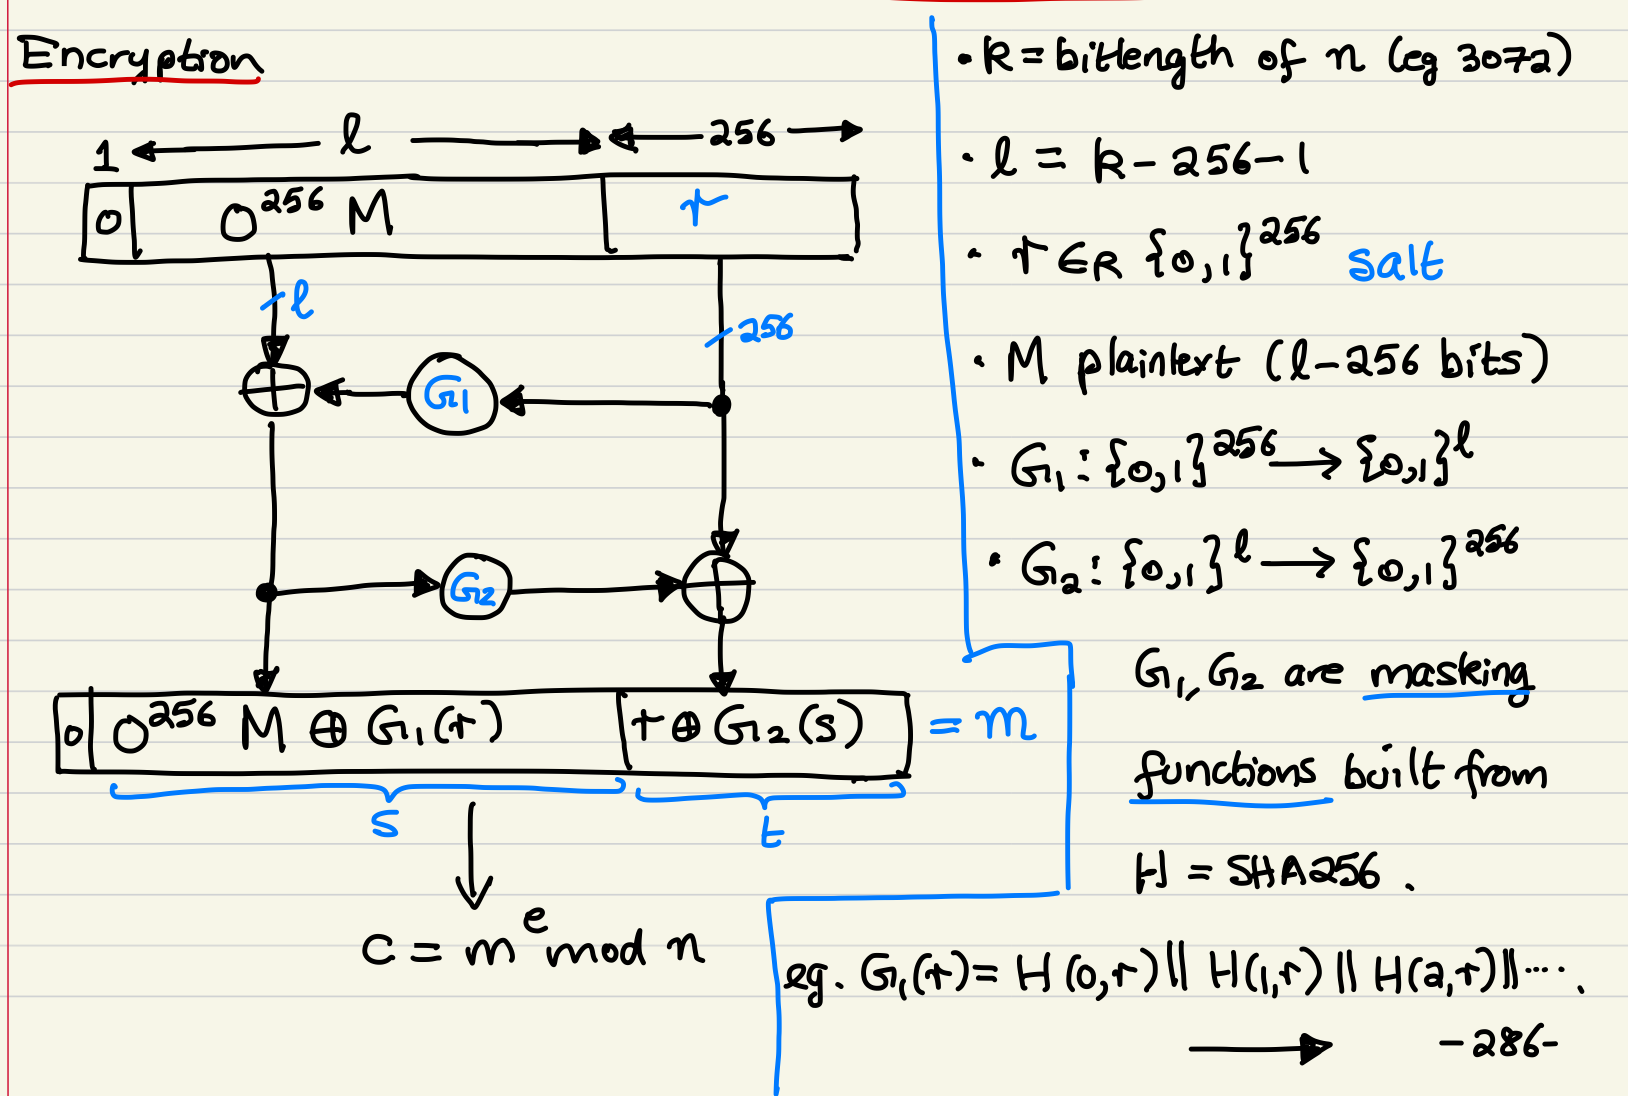
\includegraphics[width=\textwidth]{OAEP_Encryption.png}
		\caption{OAEP Encryption}
	\end{figure}
\end{center}
\begin{center}
	\begin{figure}[h!]
		\centering
		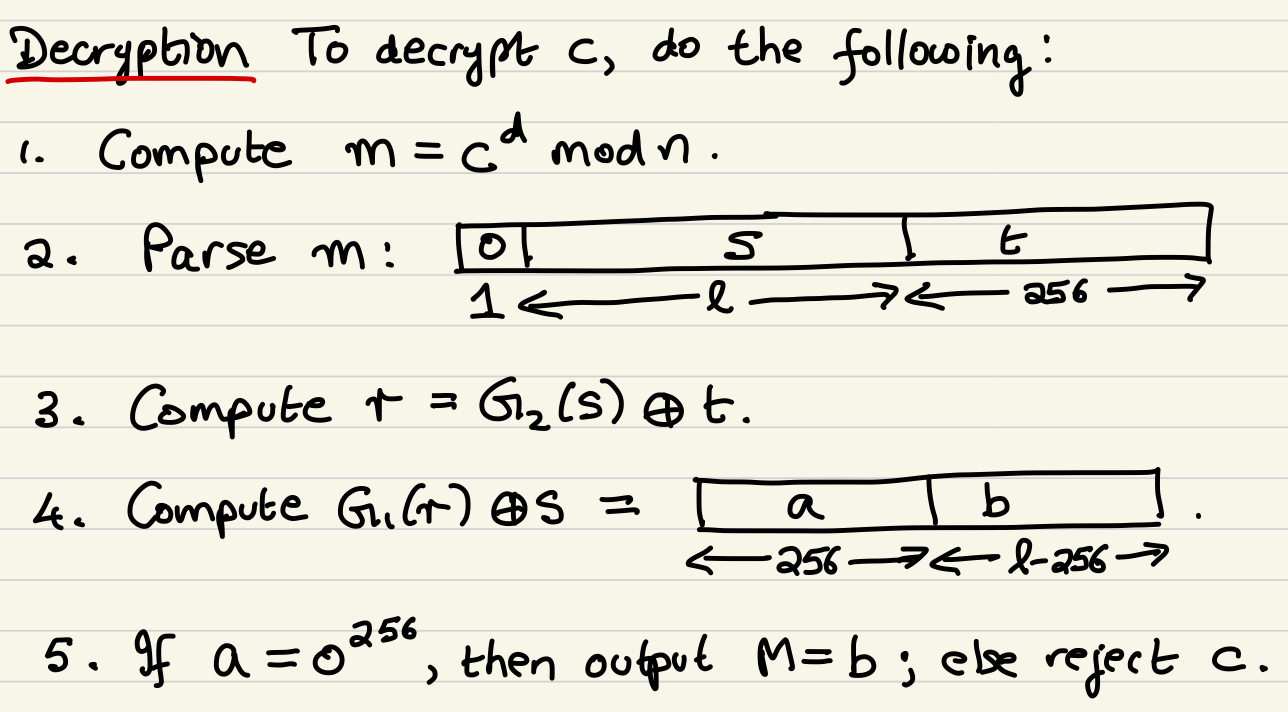
\includegraphics[width=.7\textwidth]{OAEP_Decryption.png}
		\caption{OAEP Decryption}
	\end{figure}
\end{center}
\begin{theorem}
	Suppose that RSAP is intractible, and $G_1, G_2$ are random functions. Then $RSA-OAEP$ is a secure public-key encryption scheme. 
\end{theorem}
\subsection{Status of Integer Factorization}
\subsubsection{Big-O and Little-o Notation}
Let $f(n)$ and $g(n)$ be functions from the positive integers to the positive real numbers.
\begin{definition}
	\textbf{Big-O notation}: We write $f(n) = O(g(n))$ if there exists a positive constant c and a positive integer $n_0$ such that $f(n) \leq cg(n)$ for all $n \geq n_0$.
\end{definition}

\begin{definition}
	\textbf{Little-o notation}: We write $f(n) = o(g(n))$ if $$\lim_{n \rightarrow \infty}\frac{f(n)}{g(n)} = 0$$
\end{definition}
\subsubsection{Measures of Running Time}
\begin{definition}
	\textbf{Polynomial-time algorithm} One whose worst-case running time function is of the form $O(n^c)$, where $n$ is the \textbf{input size} and $c$ is a constant.
\end{definition}
\begin{definition}
	\textbf{Exponential-time algorithm}: One whose worst-case running time function is not of the form $O(n^c)$.

	In this course, \textbf{fully exponential-time} functions are of the form $2^{cn}$, where $c$ is a constant, e.g. $O(2^{n/2})$.
\end{definition}

\begin{definition}
	\textbf{Subexponential-time algorithm} One whose worst-case running time function is of the form $2^{o(n)}$, and not of the form $O(n^c)$ for any constant $c$, e.g. $O(2^{\sqrt{n}})$.
\end{definition}

Roughly speaking, ``polynomial-time = efficient'', ``fully exponential-time = terribly inefficient'', ``subexponential-time = inefficient, but not terribly so''.

\begin{example}
	Here is an example of trial division for factoring RSA-moduli $n$: 

	We trial divide $n$ by the primes $2, 3, 5, 7, ..., \floor{\sqrt{n}}{}$. If any of these, say $\ell$, divides $n$, then stop and output the factor $\ell$ of $n$.

	The running time of this method is at most $\sqrt{n}$ trial divisions, which is $O(\sqrt{n})$

	Is this a polynomial-time algorithm for factoring RSA moduli?

	No. Since the input size is $k = O(\log n)$ and the running time is $O(\sqrt{n}) = O(n^{\frac{1}{2}}) = O(2^{\frac{k}{2}})$ since $n = 2^k$. This is a fully exponential runtime. 
\end{example}

\begin{example}
	Here is an example of subexponential time. 

	Let $A$ be an algorithm whose inputs are elements of the integers modulo $n$, $\mathbb{Z}_n$, or an integer $n$ (so the input size is $O(\log n)$).

	If the expected running time of $A$ is of the form $$L_n[\alpha, c] = O(\exp((c + o(1)(\log_e n)^\alpha)(\log_e\log_en)^{1-\alpha}))$$

	where $c$ is a positive constant, and $\alpha$ is a constant satisfying $0 < \alpha < 1$, then $A$ is subexponential-time algorithm. 

	Note that: \begin{itemize}
		\item When $\alpha = 0$, $L_n[0, c] = O((\log n)^{c + o(1)})$, which is in polytime. 
		\item When $\alpha = 1$, $L_n[0, c] = O(n^{c+o(1)})$, which is in fully exponential time. 
	\end{itemize}
\end{example}

Here are some \textbf{Special-Purpose Factoring Algorithms}: Trial division, Pollard’s $p-1$ algorithm, Pollard’s $\rho$ algorithm, elliptic curve factoring algorithm, special number field sieve.

These are only efficient if the number $n$ being factored has a \textbf{special form} (e.g., $n$ has a prime factor $p$ such that $p - 1$ has only small factors; or $n$ has a prime factor $p$ that is relatively small).

To maximize resistance to these factoring attacks on RSA moduli, one should select the RSA primes p and q \textbf{at random} and \textbf{of the same bitlength}.

\textbf{General-Purpose Factoring Algorithms}: These are factoring algorithms whose running times do not depend of any properties of the number being factored.

There have been two major developments in the history of factoring:
\begin{enumerate}
	\item (1982) \textbf{Quadratic sieve factoring algorithm (QS)}: Running time: $L_n [\frac{1}{2}, 1]$.
	\item (1990) \textbf{Number field sieve factoring algorithm (NFS)}: Running time: $L_n [\frac{1}{3}, 1.923]$.
\end{enumerate}

Recall that $$L_n[\alpha, c] = O(\exp((c + o(1)(\log_e n)^\alpha)(\log_e\log_en)^{1-\alpha}))$$

\subsubsection{History of Factoring}
\begin{center}
	\begin{tabular}{|c|c|c|c|c|}
		\hline
		Year & Number & Bits & Method & Notes\\
		\hline
		1903 & $2^{67} - 1$ & 67 & Naive & F. Cole (3 years of Sundays). In 2020: 0.02 secs in Maple\\
		\hline
		1988 & $\approx 10^{100}$ & 332 & QS & Distributed computation by 100’s of computers\\
		\hline
		1994 & RSA-129 & 425 & QS & 1600 computers around the world; 8 months\\
		\hline
		1999 & RSA-155 & 512 & NFS & 300 workstations + Cray; 5 months\\
		\hline
		2003 & RSA-174 & 576 & NFS & \\
		\hline
		2005 & RSA-200 & 663 & NFS & (55 years on a single workstation)\\
		\hline
		2009 & RSA-768 & 768 & NFS & 2000 core years\\
		\hline
		2019 & RSA-240 & 795 & NFS & 900 core years\\
		\hline
		2020 & RSA-250 & 829 & NFS & 2700 core years\\
		\hline
	\end{tabular}
\end{center}

The largest ``hard'' number factored to date is RSA-250 (250 decimal digits, 829 bits), which was factored on Feb 28 2020.

\texttt{21403246502407449612644230728393335630086147151447\\55017797754920881418023447140136643345519095804679\\61099285187247091458768739626192155736304745477052\\08051190564931066876915900197594056934574522305893\\25976697471681738069364894699871578494975937497937\\ = \\64135289477071580278790190170577389084825014742943\\44720811685963202453234463023862359875266834770873\\7661925585694639798853367\\$\times$\\33372027594978156556226010605355114227940760344767\\554666784520987023841729\\21003708025744867329688187\\7565718986258036932062711}

RSA-1024 factoring challenge (1024 bits, 309 decimal digits):

\texttt{13506641086599522334960321627880596993888147560566\\70275244851438515265106048595338339402871505719094\\41798207282164471551373680419703964191743046496589\\27425623934102086438320211037295872576235850964311\\05640735015081875106765946292055636855294752135008\\52879416377328533906109750544334999811150056977236\\890927563}

Equivalent Security Levels
\begin{center}
\begin{tabular}{|c|c|c|c|}
	\hline
	Security in bits & Block cipher & Hash Function & RSA $\log_2 n$\\
	\hline
	80 & SKIPJACK & SHA-1 & 1024\\
	\hline
	112 & Triple-DES & SHA-224 & 2048\\
	\hline
	128 & AES Small & SHA-256 & 3072\\
	\hline
	192 & AES Medium & SHA-384 & 7680\\
	\hline
	256 & AES Large & SHA-512 & 15360\\
	\hline
\end{tabular}
\end{center}

Recall that a cryptographic scheme is said to have a \textbf{security level} of $\ell$ bits if the fastest known attack on the scheme takes approximately $2^\ell$ operations

Summary: \begin{itemize}
	\item Factoring is \textbf{believed} to be a hard problem. However, we have no \textbf{proof} or \textbf{theoretical evidence} that factoring is indeed hard.
	\item However, factoring is \textbf{known} to be \textbf{easy} on a quantum computer (\textbf{Shor’s algorithm}). The largest number factored with Shor’s algorithm is the number \textbf{21}. The big open question is whether large-scale quantum computers can ever be built.
	\item 512-bit RSA is considered insecure today
	\item 1024-bit RSA is considered risky today (but still deployed)
	\item Applications are \textbf{moving} to \textbf{2048-bit} and \textbf{3072-bit} RSA.
\end{itemize}
\subsection{RSA Signature Scheme}
\subsubsection{Basic RSA Signature Scheme}
\newpage
\begin{algorithm}
	Each entity Alice does the following: \\
	Randomly select two large distinct primes $p, q$ of the same bit length. (This can be done efficiently)\\
	Compute $n = pq$ and $\phi = \phi(n) = (p-1)(q-1)$\\
	Select an arbitrary integer $e$ such that $1 < e < \phi$ and $\gcd(\phi, e) = 1$\\
	Compute the integer $d$, $1 < d < \phi$, with $ed \equiv 1 \pmod \phi$\\
	Alice's public key is $(n, e)$; her private key is $d$
	\caption{Key Generation of RSA Signature Scheme}
\end{algorithm}

\begin{algorithm}
	To sign a message $m \in \{0,1\}^*$, $A$ does the following: \\
	Compute $M = H(m)$, where $H$ is a hash function\\
	Compute $s = M^d \mod n$ (so $s^e \equiv M^{ed} \equiv M \mod n$)\\
	$A$'s signature on $m$ is $s$ (the signed message $(m, s)$)
	\caption{Signature Generation of RSA Signature Scheme}
\end{algorithm}

\begin{algorithm}
	To verify $A$'s signature $s$ on $m$, $B$ does the following: \\
	Obtain an authentic copy of $A$'s public key $(n, e)$\\
	Compute $M = H(m)$\\
	Compute $M' = s^e \mod n$\\
	Accept $(m,s)$ if and only if $M = M'$
	\caption{Signature Verification of RSA Signature Scheme}
\end{algorithm}
\subsubsection{Security of RSA Signature Scheme}
\textbf{Hardness of RSAP}: 

We require that RSAP be intractible, since otherwise $E$ could forge $A$'s signature as follows: \begin{enumerate}
	\item Select arbitrary $m$
	\item Compute $M = H(m)$
	\item Solve $s^e \equiv M \pmod n$ for $s$
	\item Then $s$ is $A$'s signature on $m$
\end{enumerate}

\textbf{Security Properties of the Hash Function}: 

\textbf{\textcolor{blue}{Preimage Resistance}}: If $H$ is not preimage resistant, and the range of $H$ is $[0, n-1]$, $E$ can forge signatures as follows: \begin{enumerate}
	\item Select $s \in_R [0,n-1]$
	\item Compute $M = s^e \mod n$
	\item Find $m$ such that $H(m) = M$
	\item Then $s$ is $A$'s signature on $m$
\end{enumerate}

\textbf{\textcolor{blue}{2nd Preimage Resistance}}: If $H$ is not 2nd preimage resistant, $E$ can forge signatures as follows: \begin{enumerate}
	\item Suppose $(m,s)$ is a valid signed message
	\item Find an $m'$, $m \neq m'$ such that $H(m) = H(m')$
	\item Then $(m', s)$ is a valid signed message
\end{enumerate}

\textbf{\textcolor{blue}{Collision Resistance}}: If $H$ is not collision resistant, $E$ can forge signatures as follows: \begin{enumerate}
	\item Select $m_1, m_2$ such that $H(m_1) = H(m_2)$ where $m_1$ and $m_2$ are two distinct messages
	\item Induce $A$ to sign $m_1$: $s = H(m_1)^d \mod n$
	\item Then $s$ is also $A$'s signature on $m_2$
\end{enumerate}

\textbf{Objectives of the Adversary}: 
\begin{enumerate}
	\item \textbf{Total Break}: $E$ recovers $A$'s private key, or a method for systematically forging $A$'s signatures (i.e. $E$ can compute $A$'s signature for arbitrary messages)
	\item \textbf{Existential Forgery}: $E$ forges $A$'s signature for a single message; $E$ may not have any control over the content or structure of this message. 
\end{enumerate}

\textbf{Attack Model}: 
Types of attacks $E$ can launch: \begin{enumerate}
	\item \textbf{Key-only attack}: The only information $E$ has is $A$'s public key
	\item \textbf{Known-message attack}: $E$ knows some message/signature pairs
	\item \textbf{Chosen-message attack}: $E$ has access to a signing oracle which it can use to obtain $A$'s signature on some messages of its choosing
\end{enumerate}
\textbf{Security Definition}: 
\begin{definition}
	A signature scheme is said to be \textbf{secure} if it is existentially unforgeable by a computationally bounded adversary who launches a chosen-message attack 
\end{definition}
Note: the adversary has access to a signing oracle. Its goal is to compute a single valid message/signature pair for any message that was not previously given to the signing oracle.

Is the basic RSA signature scheme secure?\begin{itemize}
	\item No if $H$ is SHA-256
	\item Yes if H is a ``full domain'' hash function.
\end{itemize}
\subsubsection{Full Domain Hash RSA (RSA-FDH)}
It's the same as the basic RSA signature scheme, except that the hash function is $$H : \{0, 1\}^* \rightarrow [0, n - 1]$$

In practice, one could use: $$H(m) = SHA-256(1, m) \| SHA-256(2, m) \| \cdots \| SHA-256(t, m)$$
\begin{theorem}
	\textbf{Bellare \& Rogaway, 1996}: If RSAP is intractable and $H$ is a random function, then RSA-FDH is a secure signature scheme.
\end{theorem}
\subsubsection{RSA PKCS \#1 v1.5 Signatures}
PKCS stands for public key cryptographic standards. 

\begin{center}
	\begin{figure}[h!]
		\centering
		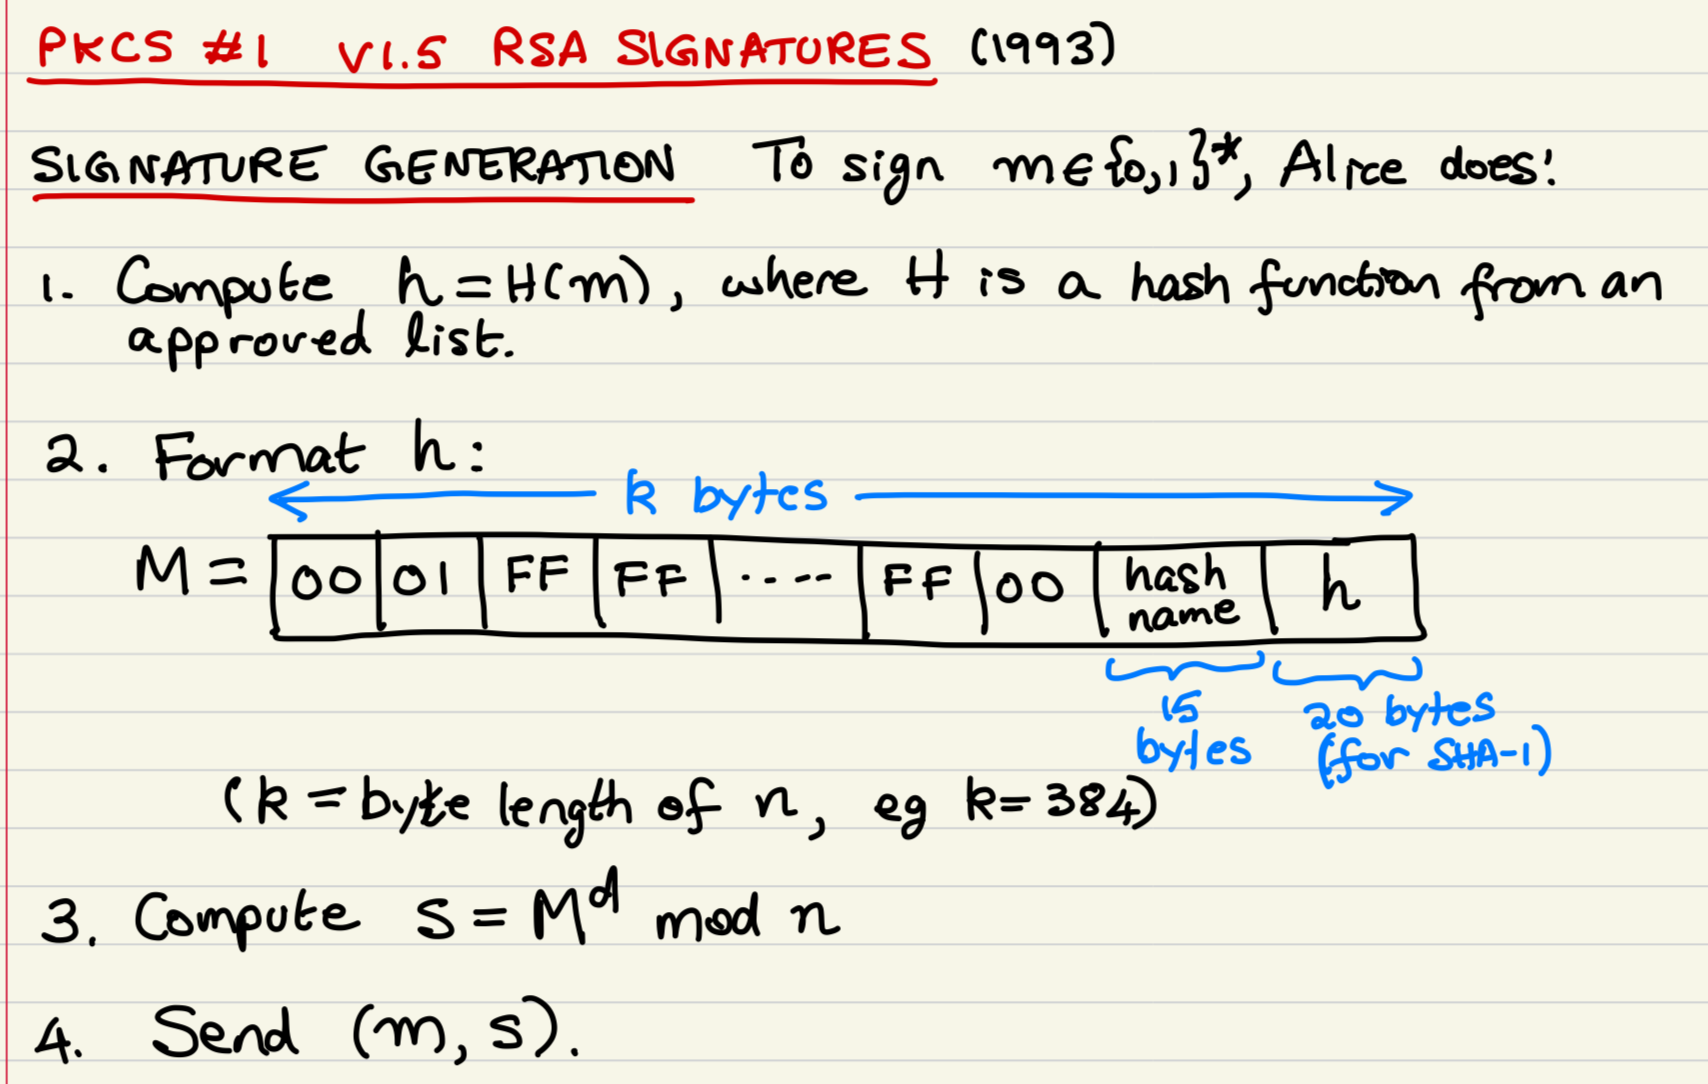
\includegraphics[width=.9\textwidth]{PKCS_Signature_Generation.png}
		\caption{PKCS Signature Generation}
	\end{figure}
\end{center}

\begin{center}
	\begin{figure}[h!]
		\centering
		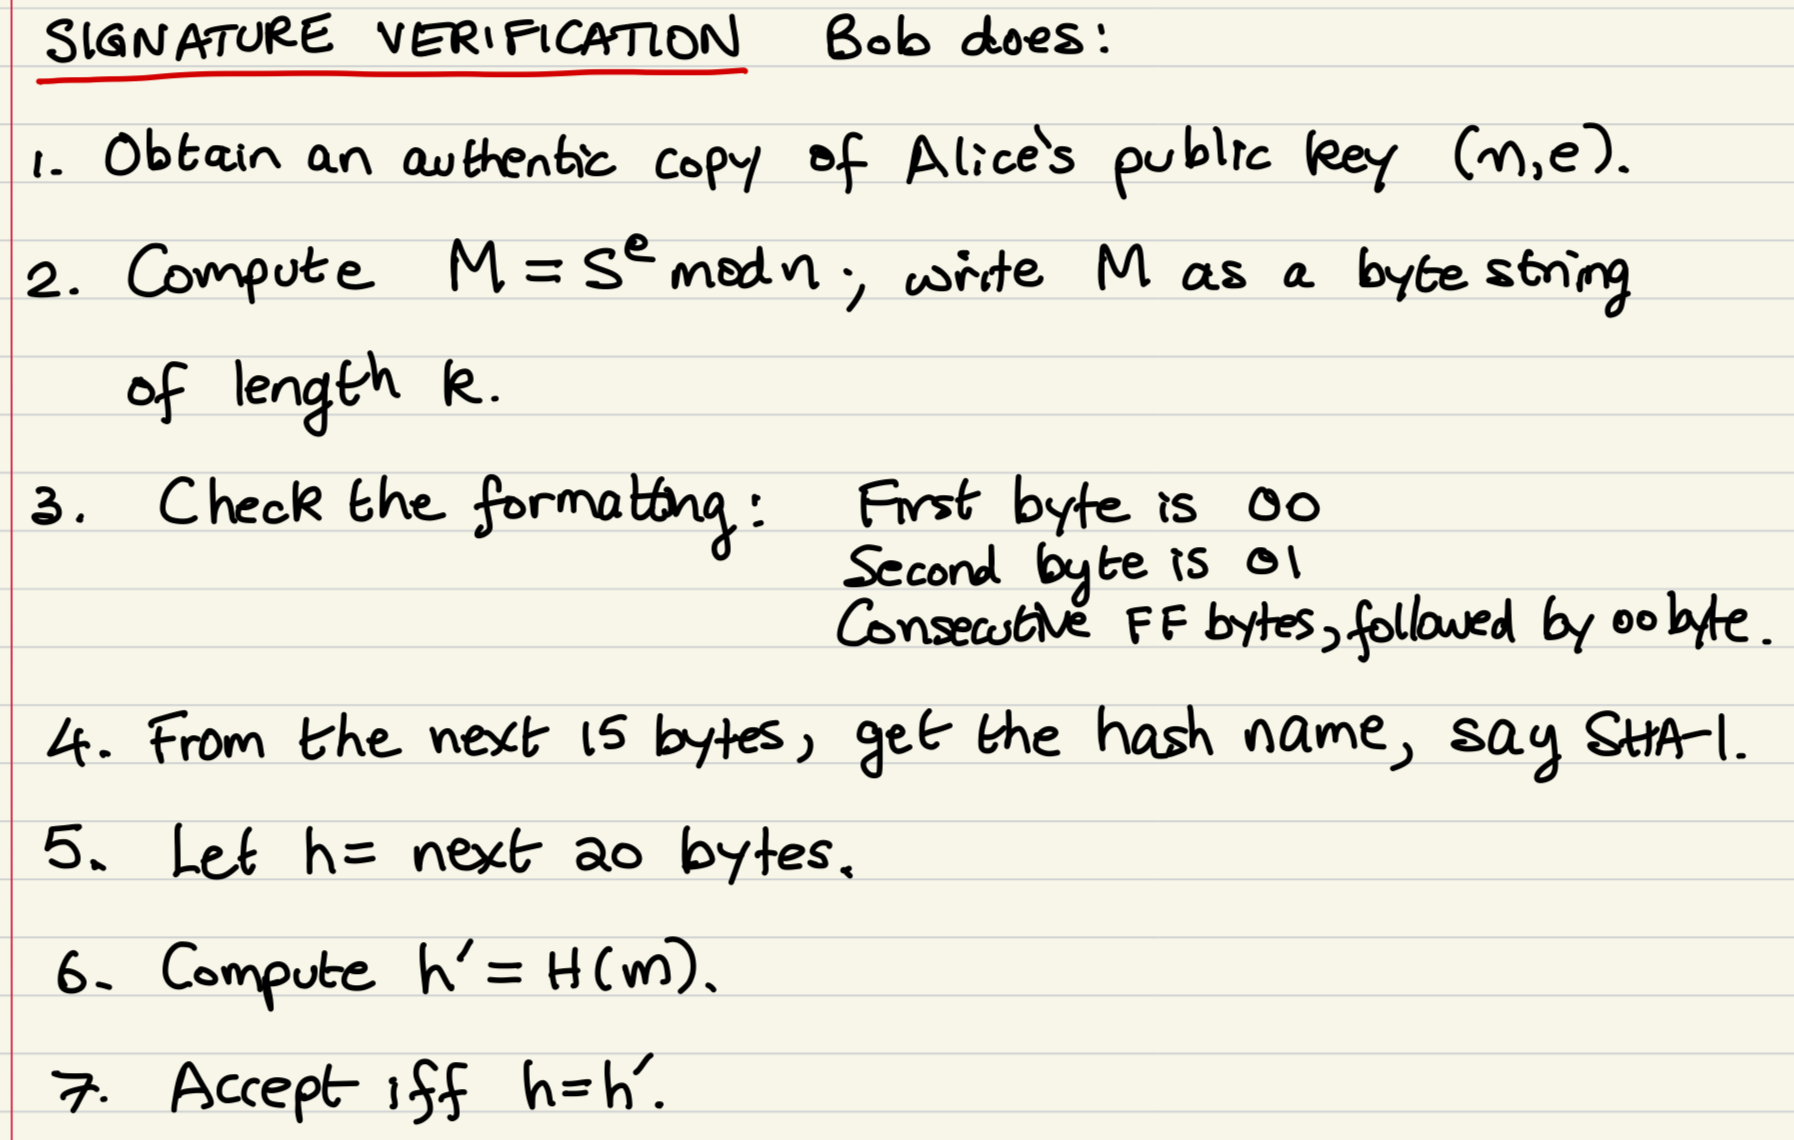
\includegraphics[width=.9\textwidth]{PKCS_Signature_Verification.png}
		\caption{PKCS Signature Verification}
	\end{figure}
\end{center}

\begin{center}
	\begin{figure}[h!]
		\centering
		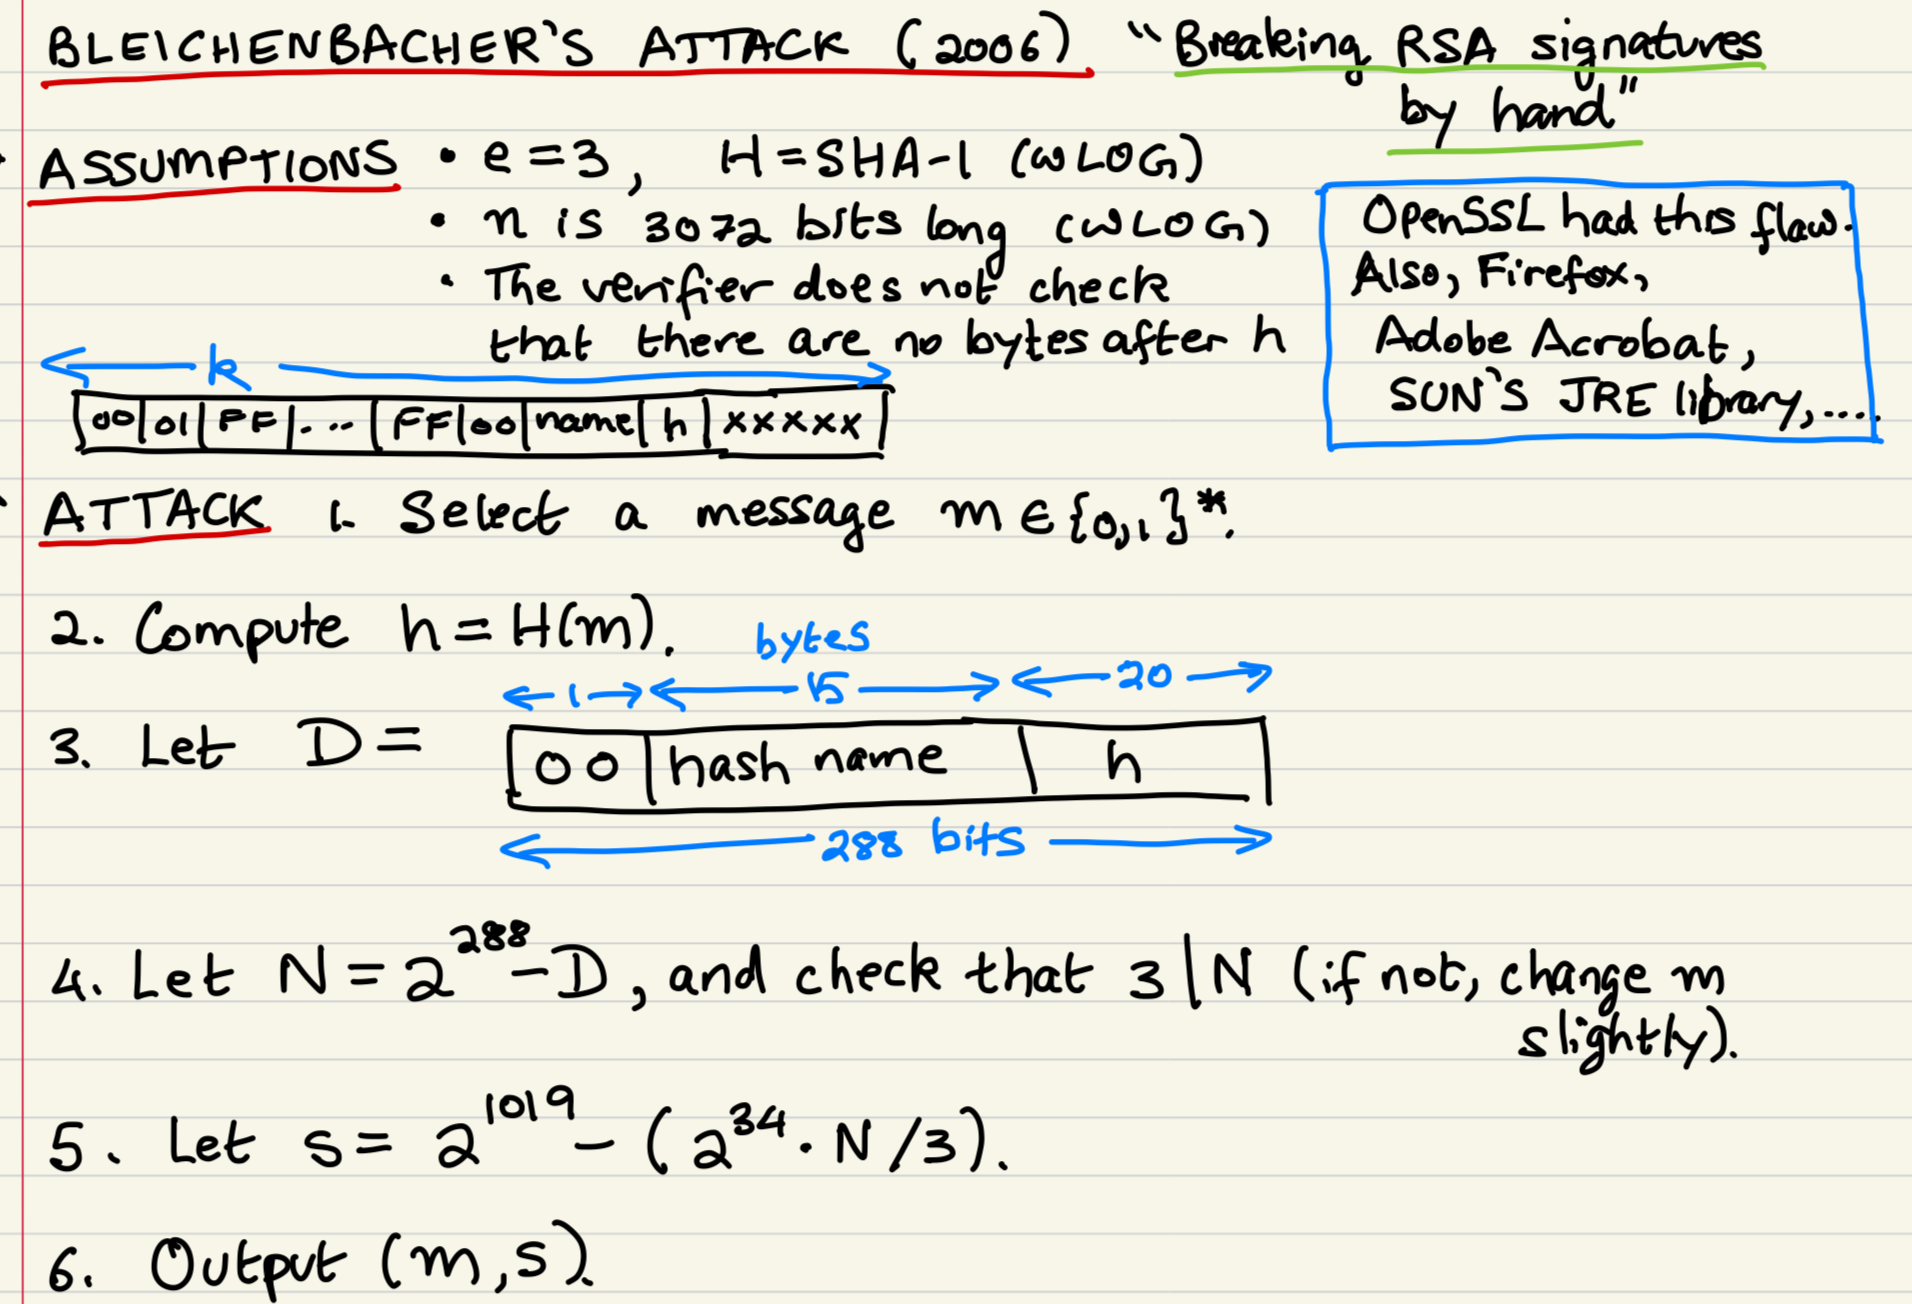
\includegraphics[width=.9\textwidth]{PKCS_Bleichenbacher's_Attack.png}
		\caption{PKCS Bleichenbacher's Attack}
	\end{figure}
\end{center}

\begin{center}
	\begin{figure}[h!]
		\centering
		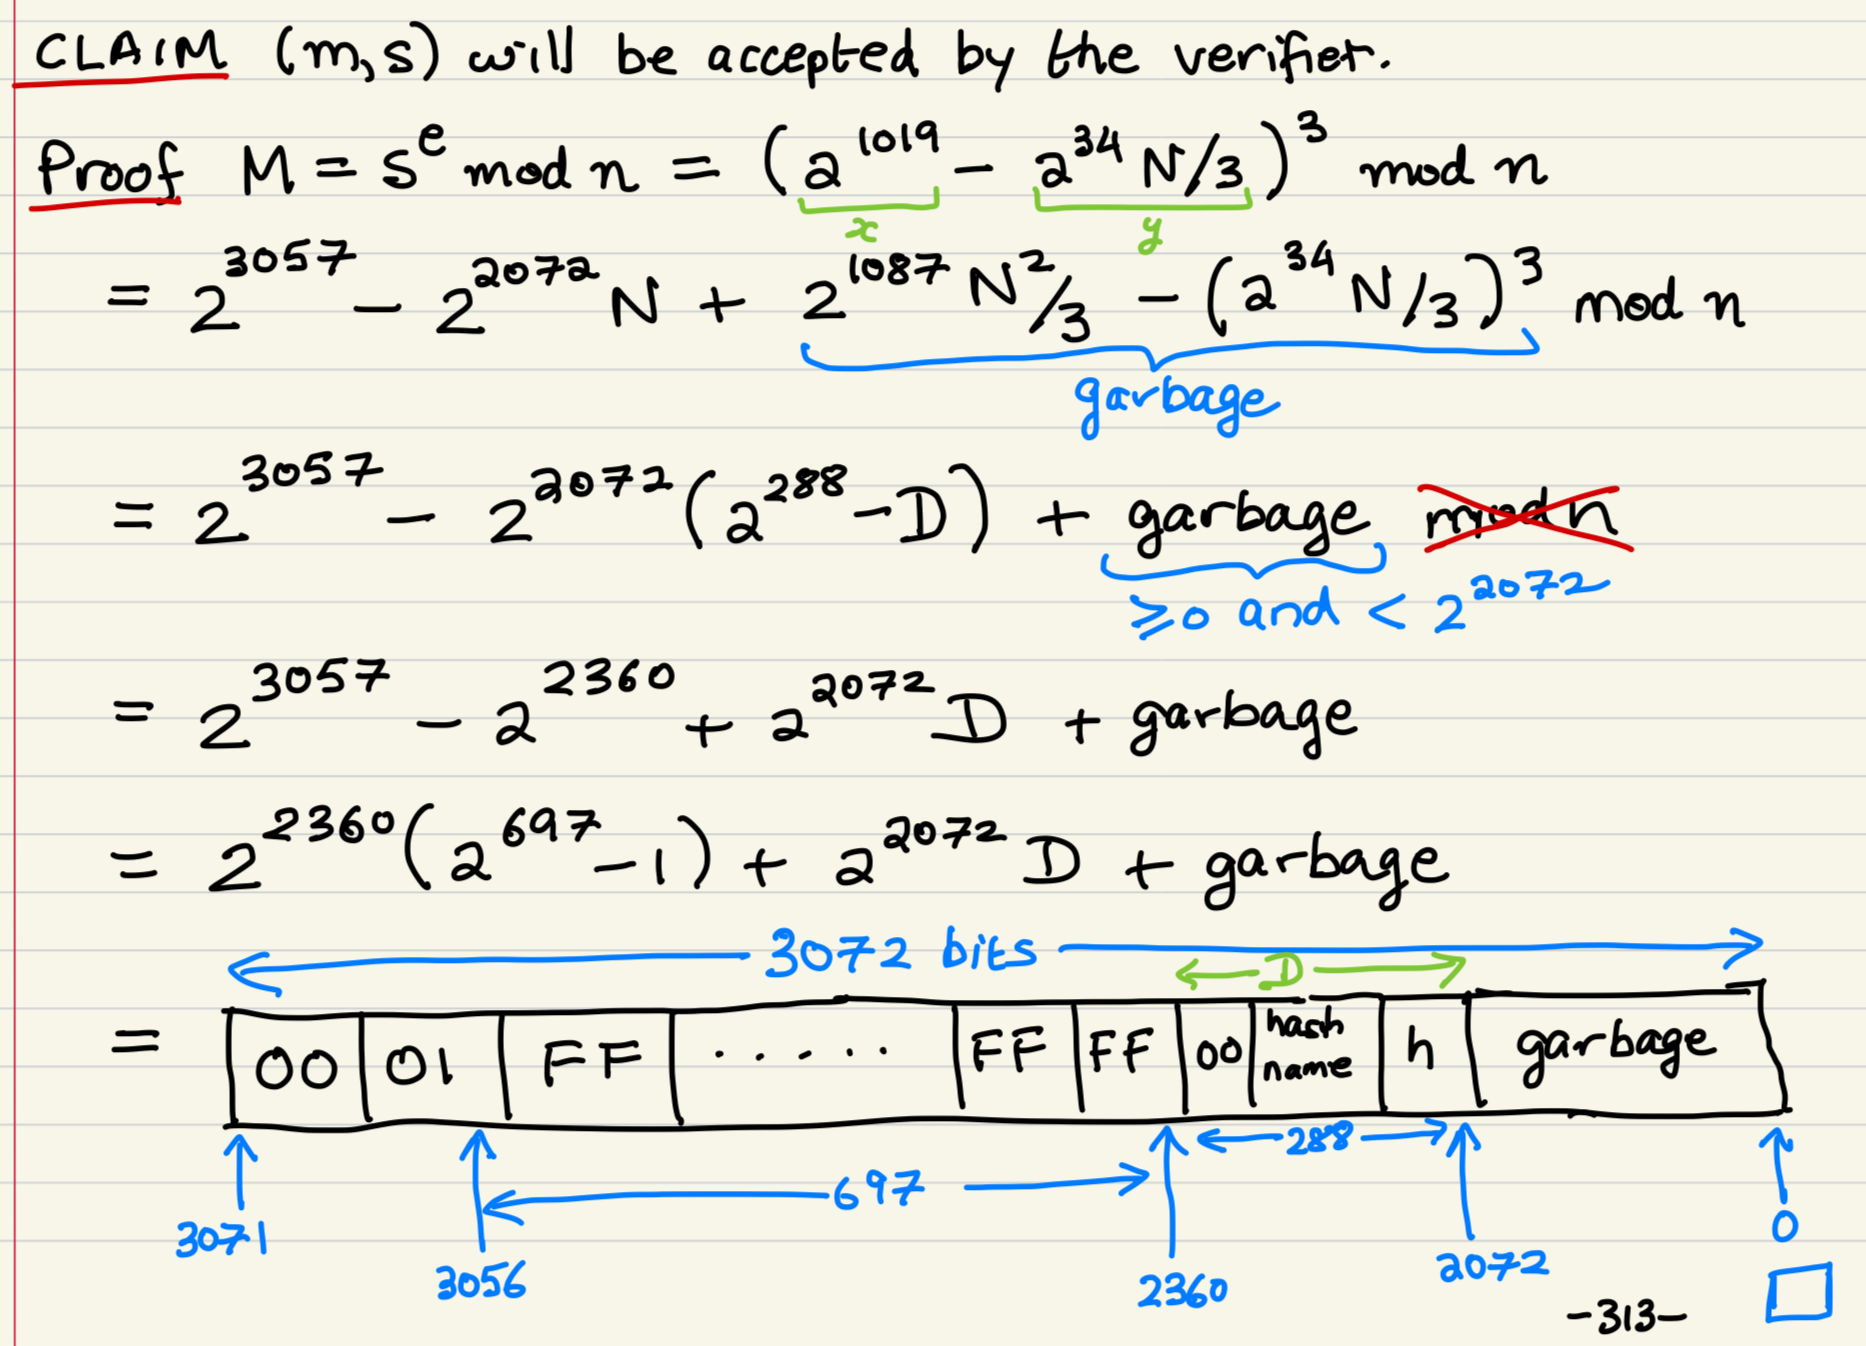
\includegraphics[width=\textwidth]{PKCS_Bleichenbacher's_Attack_Correctness.png}
		\caption{PKCS Bleichenbacher's Attack Correctness}
	\end{figure}
\end{center}

% Section 8
\section{Elliptic Curve Cryptography}
\subsection{Elliptic Curves}

\begin{center}
	\begin{figure}[h!]
		\centering
		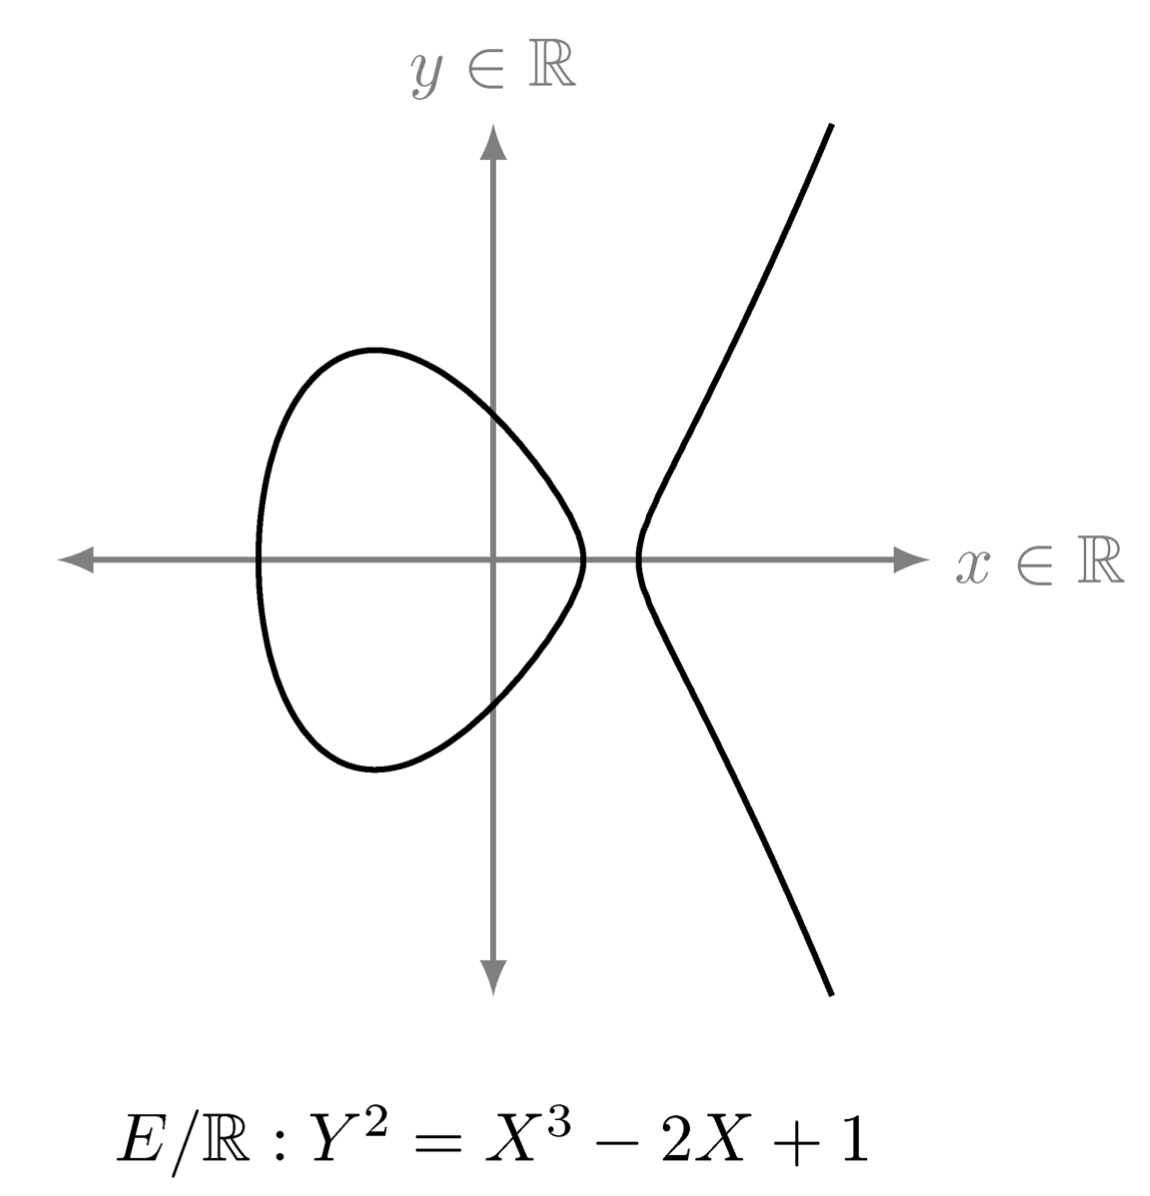
\includegraphics[width=.4\textwidth]{Elliptic_Curves.png}
		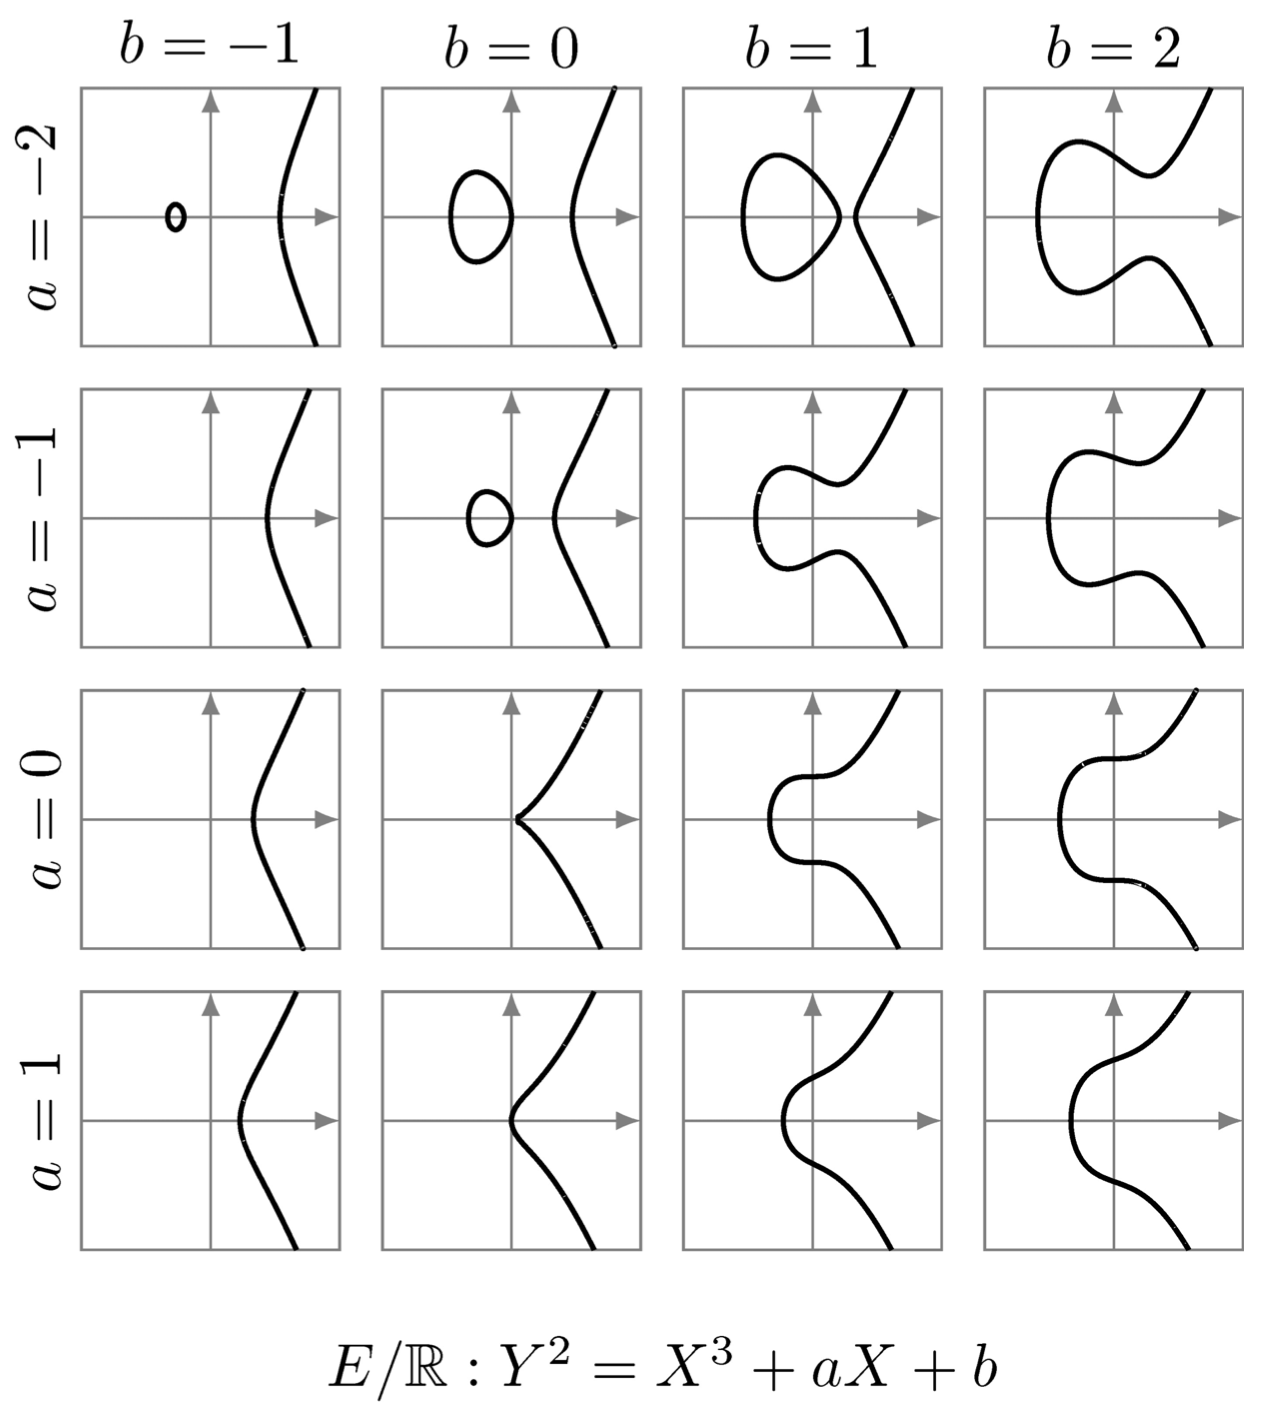
\includegraphics[width=.4\textwidth]{Elliptic_Curves_2.png}
		\caption{Elliptic Curves}
	\end{figure}
\end{center}
\begin{center}
	\begin{figure}[h!]
		\centering
		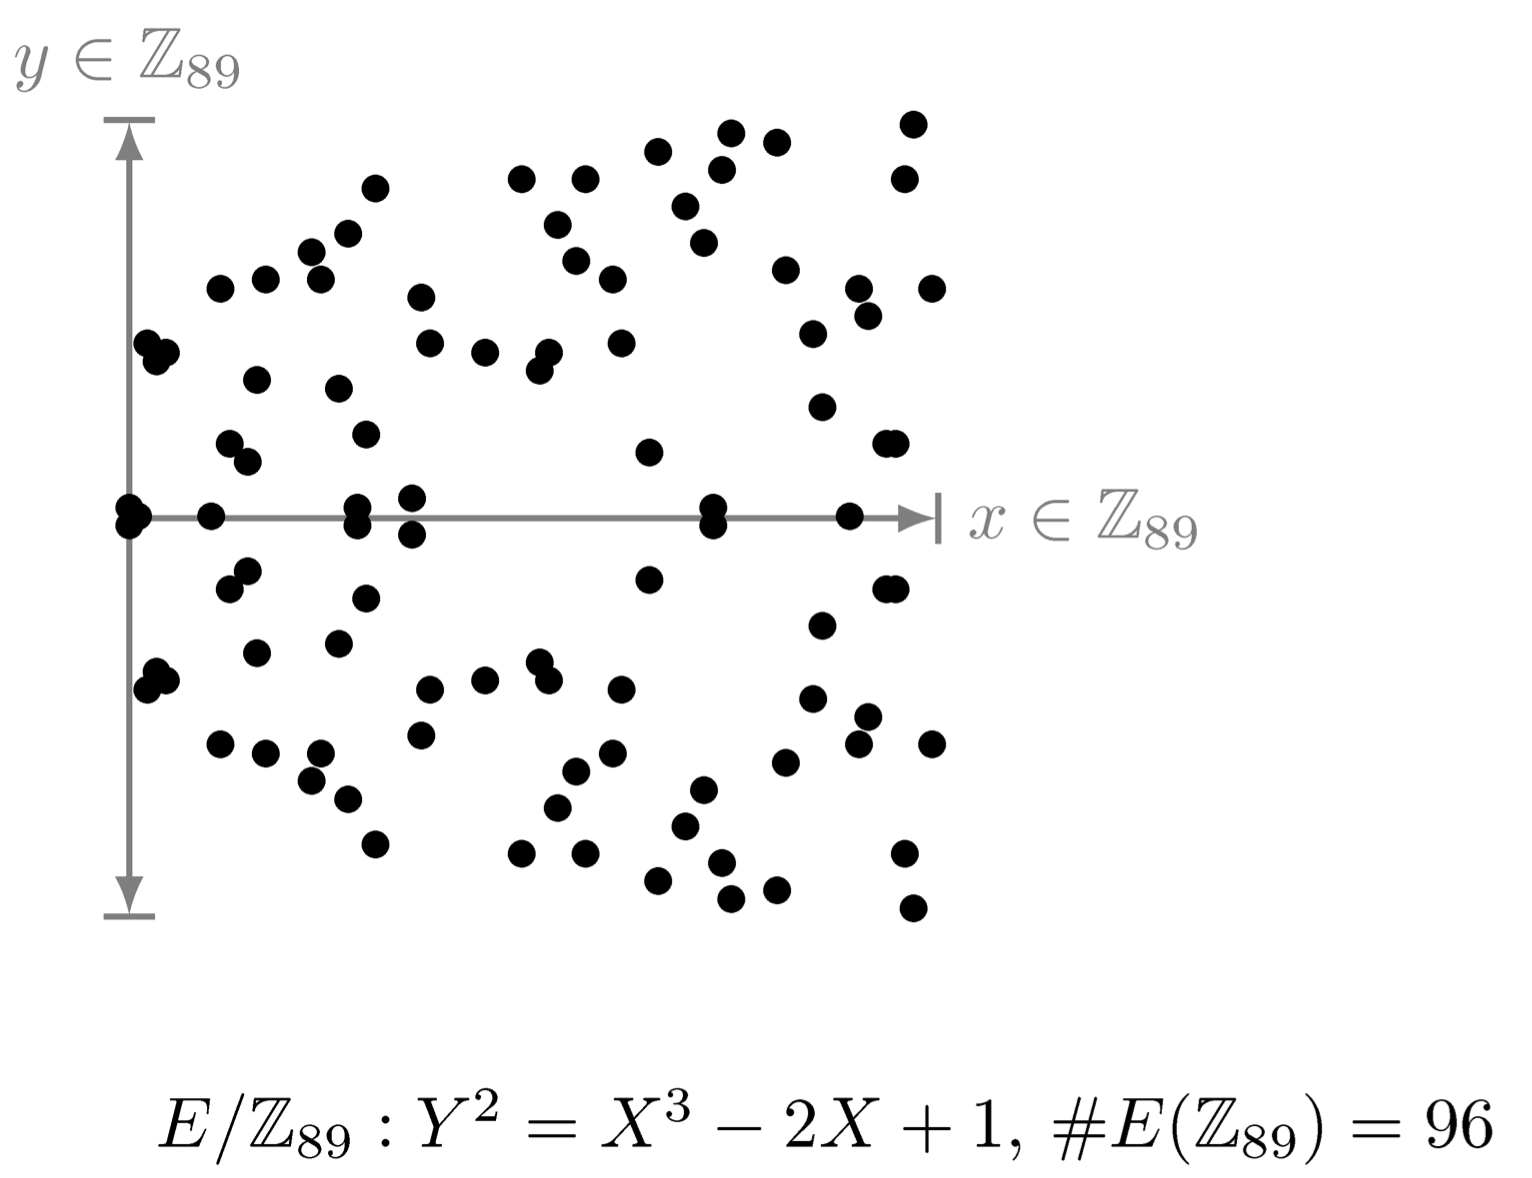
\includegraphics[width=.6\textwidth]{Elliptic_Curves_Z89.png}
		\caption{Elliptic Curves over Finite Fields}
	\end{figure}
\end{center}

Let $F = \mathbb{R}$ or $F = \mathbb{Z}_p$ (where $p \geq 5$ is prime)
\begin{definition}
	An \textbf{elliptic curve $E$ over $F$} is defined by an equation $$E / F = Y^2 = X^3 + aX + b$$ where $a, b \in F$ with $4a^3 + 27b^2 \neq 0$
\end{definition}

\begin{definition}
	The set of $F$-rational points on $E$ is $$E(F) = \{(x, y) \in F \times F : y^2 = x^3 + ax+b\} \cup \{\infty\}$$ where $\infty$ is a special point called \textbf{the point at infinity}.
\end{definition}
Here are some examples of elliptic curves. 
\begin{center}
	\begin{figure}[h!]
		\centering
		\includegraphics[width=\textwidth]{Elliptic_Curves_Example.png}
		\caption{Elliptic Curves Examples}
	\end{figure}
\end{center}
\begin{example}
	Now, consider $E / \mathbb{Z}_{11}: Y^2 = X^3 + X + 6$. Then $$E(\mathbb{Z}_{11}) = \{\infty, (2,4), (2,7), (3,5),(3,6),(5,2),(5,9),(7,2),(7,9),(8,3),(8,8),(10,2),(10,9)\}$$
	So $\#E(\mathbb{Z}_{11} = 13)$. Note that $\# S$ is the cardinality of $S$
\end{example}
Note that $\#E(\mathbb{Z}_p)$ is finite. It is easy to see that $1 \leq \#E(\mathbb{Z}_p) \leq 2p+1$. In fact, we have the following theorem: 
\begin{theorem}
	\textbf{Hasse's Theorem}: Let $E$ be an elliptic curve defined over $\mathbb{Z}_p$. Then $$(\sqrt{p} - 1)^2 \leq \#E(\mathbb{Z}_p) \leq (\sqrt{p}+1)^2$$

	Hence, $\#E(\mathbb{Z}_p) \approx p$
\end{theorem}

\textbf{Point Addition}: There is a ``natural'' way to add two points in $E(F)$ to get a third point in $E(F)$

\textbf{Geometric Description of the Addition Rule}: Let $E$ be an elliptic curve over $\mathbb{R}$. Think of $\infty$ as an imaginary point through which every vertical line passes (in either direction)

The geometric rule is: Let $P, Q \in E(F)$. Let $T \in E(F)$ be the third point of intersection of the line $\ell$ through $P$ and $Q$ with the elliptic curve. Then $P + Q$ is the reflection of $T$ in the $X$-axis.  

\begin{center}
	\begin{figure}[h!]
		\centering
		\includegraphics[width=.3\textwidth]{Elliptic_Curves_Geometric_Rule.png}
		\caption{Elliptic Curves Geometric Rule Description}
	\end{figure}
\end{center}


\begin{center}
	\begin{figure}[h!]
		\centering
		\includegraphics[width=\textwidth]{Elliptic_Curves_Addition_Rule.png}
		\caption{Elliptic Curves Addition Rules}
	\end{figure}
\end{center}
\begin{proposition}
	The geometric rules of elliptic curves are defined as follows: 

	Let $E$ be an elliptic curve defined over $F$: \begin{enumerate}
		\item [A1: ] $P + \infty = \infty + P = P$ for all $P \in E(F)$
		\item [A2: ] If $P = (x, y) \in E(F)$, then $-P = (x, -y)$; also $-\infty = \infty$. Also, $P + (-P) = (-P) + P = \infty$, for all $P \in E(F)$
		\item [A3: ] Let $P = (x_1, y_1), Q = (x_2, y_2) \in E(F)$, with $P \neq \pm Q$. Then $P + Q = (x_3, y_3)$ where $$x_3 = \lambda^2 - x_1 - x_2\;\;\;\;\;\; y_3 = -y_1 + \lambda(x_1 - x_3)\;\;\;\;\;\; \lambda = \frac{y_2 - y_1}{x_2 - x_1}$$
		\item [A4: ] Let $P = (x_1, y_1) \in E(F)$ with $P \neq -P$. Then $P + P = (x_3, y_3)$ where $$x_3 = \lambda^2 - 2x_1\;\;\;\;\;\; y_3 = -y_1 + \lambda(x_1 - x_3)\;\;\;\;\;\; \lambda = \frac{3x_1^2 + a}{2y_1}$$
	\end{enumerate}
\end{proposition}
\begin{proof}
	Derivation of the addition formula in A3 above: 

	Let $P = (x_1, y_1), Q = (x_2, y_2) \in E(F)$ with $P \neq \pm Q$

	The equation of the line $\ell$ through $P$ and $Q$ is $\ell: Y = y_1 + \lambda(X - x_1)$, denote it as \textcolor{blue}{$(*)$}, where $\lambda = \frac{y_2 - y_1}{x_2 - x_1}$ is the slope of $\ell$

	To find the third point of intersection of $\ell$ with $E$, we substitute \textcolor{blue}{$(*)$} into the equation for $E: Y^2 = X^3 + aX +b$ to get: $$[y_1 + \lambda(X-x_1)]^2 = X^3 + aX + b$$
	So $$X^3 + aX + b - [y_1 + \lambda(X-x_1)]^2 = 0$$
	This equation has two solutions in $F$, namely $x_1$ and $x_2$. Thus, it must have a third solution in $F$, say $x_3$. Thus, we have $$X^3 + aX + b - [y_1 + \lambda(X-x_1)]^2 = (X - x_1)(X - x_2)(X - x_3)$$
	Equating coefficients of $X^2$ of both sides gives $$-\lambda^2 = -(x_1 + x_2+x_3)$$ So $$x_3 = \lambda^2 - x_1 - x_2$$
	The coordinates of $T$ are $(x_3, y_3')$, where $y_3' = y_1 + \lambda(x_3 - x_1)$. Hence, the coordinates of $P + Q$ are $(x_3, y_3) = (x_3, -y_3')$ so $$y_3 = -y_1 + \lambda(x_1 - x_3)$$

	For derivation of the addition formula in A4, the process is similar. The slope of the tangent line $\ell$ at $P = (x_1, y_1)$ is $\lambda = \frac{3x_1^2 + a}{2y_1}$. 
	
	Also, $E: Y^2 = X^3 + aX + b$, we can compute derivatives: $2Y \cdot \frac{dY}{dX} = 3X^2 + a$, so $\frac{dY}{dX} = \frac{3X^2 + a}{2Y}$
\end{proof}

\begin{example}
	Consider the elliptic curve $E / \mathbb{Z}_{11}: Y^2 = X^3 + X + 6$. The set of $\mathbb{Z}_{11}$-rational points on $E$ is $$E(\mathbb{Z}_{11}) = \{\infty, (2,4), (2,7), (3,5),(3,6),(5,2),(5,9),(7,2),(7,9),(8,3),(8,8),(10,2),(10,9)\}$$

	$$(2,4) + (2,7) = \infty$$
	$$(2,4) + (8,3) = (5,2)$$
	$$(2,4) + (2,4) = (5,9)$$
\end{example}

In fact, $(E(F), +)$ is an abelian group. In particular, the addition rule satisfies the following properties: \begin{enumerate}
	\item [P1: ] $P + \infty = \infty + P = P$ for all $P \in E(F)$
	\item [P2: ] For each $P \in E(F)$, there exists $Q \in E(F)$ such that $P + Q = Q + P = \infty$
	\item [P3: ] $P + Q = Q + P$ for all $P, Q \in E(F)$
	\item [P4: ] $(P+Q)+R = P+(Q+R)$ for all $P,Q,R \in E(F)$ 
\end{enumerate}

\subsection{Elliptic Curves Discrete Logarithm Problem(ECDLP)}
Let $E: Y^2 + X^3 + aX + b$ be an elliptic curve defined over $F = \mathbb{Z}_p$. Let $n = \#(\mathbb{Z}_p)$ and suppose that $n$ is a prime. Note: $n \approx p$ by Hasse's Theorem.

\begin{definition}
	Let $P \in E(\mathbb{Z}_p)$ and let $k \in \mathbb{N}$. Then, $kP = \underbrace{P + P + \cdots + P}_{k}$. Also $0P = \infty$ and $(-k)P = -(kP)$. This operation is called \textbf{point multiplication}. 
\end{definition}

\begin{theorem}
	Let $P \in E(\mathbb{Z}_p)$, $P \neq \infty$. Then: \begin{enumerate}
		\item $nP = \infty$
		\item The points $\infty, P, 2P, \cdots, (n-1)P$ are distinct, and so $E(\mathbb{Z}_p) = \{\infty, P, 2P, \cdots, (n-1)P\}$. $P$ is called a generator of $E(\mathbb{Z}_p)$
	\end{enumerate}
\end{theorem}

\begin{definition}
	The \textbf{elliptic curve discrete logarithm problem(ECDLP)} is the following: 
	
	Given $E, p, n, P \in E(\mathbb{Z}_p)$ (with $P \neq \infty$), and $Q \in E(\mathbb{Z}_p)$. Find the integer $\ell \in [0, n-1]$ such that $Q = \ell p$. The integer $\ell$ is called the \textbf{discrete logarithm} of $Q$ to the base $P$, written $\ell = \log_pQ$
\end{definition}
We have several approaches to this problem: 
\textbf{Brute Force}: The ECDLP can be solved by computing $P, 2P, 3P, ...$ until $Q$ is encountered. This attack takes time $O(n)$ point additions, or $O(p)$ additions (recall that $n \approx p$). 
	
This is \textbf{fully exponential} since an ECDLP instance has size $O(\log p)$ bits

\textbf{Shank's algorithm} (for solving ECDLP): Idea. Let $m = \floor{\sqrt{n}}{}$ By the division algorithm, there exists unique integers $q, r$ with $\ell = qm + r$, where $0 \leq r < m$ and $0 \leq q < m$. Hence, $\ell - qm = r$. Multiplying both sides by $P$ gives $$\ell P - qmP = rP$$ so $Q-q(mP) = rP$ 

This equation suggests the following algorithm for finding $\ell = \log_p Q$: \begin{enumerate}
	\item For each $e \in [0, m-1]$, compute $rP$ and store $(rP,r)$ in a sorted table
	\item Compute $M = mP$
	\item For each $q \in [0, m-1]$, compute $R = Q-qM$ and look it up in the table. If $R = rP$, then output ``$\ell = qm+r$'' and STOP
\end{enumerate}
Runtime: $O(m) = O(\sqrt{n}) = O(\sqrt{p})$ point additions. 

Storage: $O(\sqrt{p})$ points

\textbf{Pollard's algorithm}: The ECDLP can be solved in time $O(\sqrt{p})$ point additions and negligible storage. Moreover, VW collision research can be used to perfectly parallelize Pollard's algorithm. 

Note that Pollard's algorithm is the fastest method known for solving the ECDLP (except for some very special elliptic curves that can easily be avoided in practice).

\textbf{Shor's algorithm}: The ECDLP can be solved in polynomial time on a quantum computer

\subsection{Elliptic Curves Cryptography}
It is invented by Neal Koblitz and Victor Miller. Why do we want Elliptic Curves Cryptography? \begin{itemize}
	\item [RSA: ] Security is based on intractability of \textbf{integer factorization}. Fastest known attacks take \textbf{subexponential time}. 
	\item [ECC: ] Security is based on intractability of \textbf{ECDLP}. Fastest known attacks take \textbf{fully exponential time}. 
\end{itemize}

Hence, elliptic curve cryptographic systems can use \textbf{smaller parameters} than their RSA counterparts, while achieving the same security level. Smaller parameter leads to faster implementation and smaller public keys and signature sizes. 

\begin{center}
\begin{tabular}{|c|c|c|}
	\hline
	Security Level & Bitlength of RSA $n$ & Bitlength of ECC $p$\\
	\hline
	80 & 1024 & 160\\
	112 & 2048 & 224\\
	128 & 3072 & 256\\
	192 & 7680 & 384\\
	256 & 15360 & 512\\
	\hline
\end{tabular}
\end{center}

Deployment of ECC generally use an elliptic curve that has been standardized (by NIST). Examples include \texttt{P-256}, \texttt{Curve25519}, \texttt{P-384}. 

\subsubsection{P-256 Elliptic Curve}
\begin{itemize}
	\item P-256 is an elliptic curve chosen by the National Security Agency in 1998 for U.S. government use.
	\item P-256 should be used for applications that require the \textbf{128-bit security level}.
	\item $p = 2^{256} - 2^{224} + 2^{192} + 2^{96} - 1$ is prime.
	\item P-256 is the elliptic curve $E : Y^2 = X^3 - 3X + b$ over $\mathbb{Z}_p$, where $b = $
	\begin{verbatim}
		410583637251521421293261297800472684091
		14441015993725554835256314039467401291
	\end{verbatim}
	\item We have $n = \#E(\mathbb{Z}_p)$ is prime, where $n = $
	\begin{verbatim}
		115792089210356248762697446949407573529
		996955224135760342422259061068512044369
	\end{verbatim}
\end{itemize}

\subsubsection{Curve25519}
\begin{itemize}
	\item Selected by \textbf{Dan Bernstein} in 2005, and developed with \textbf{Tanja Lange} and others.
	\item Curve25519 should be used for applications that require the  \textbf{128-bit security level}.
	\item $p = 2^{255} - 19$ is prime.
	\item Curve25519 is the elliptic curve $E : Y^2 = X^3 + 486662X^2 + X$ over $\mathbb{Z}_p$. The curve is in ``Montgomery form''.
	\item We have $n = \#E(\mathbb{Z}_p) = 8n$, where $n$ is the following 253-bit prime $$2^{252} + 27742317777372353535851937790883648493$$
\end{itemize}

\subsubsection{P-384 Elliptic Curve}
\begin{itemize}
	\item P-384 is an elliptic curve chosen by the National Security Agency in 1998 for U.S. government use.
	\item P-384 should be used for applications that require the \textbf{192-bit security level}.
	\item $p = 2^{384} - 2^{128} - 2^{96} + 2^{32} - 1$ is prime.
	\item P-384 is the elliptic curve $E : Y^2 = X^3 - 3X + b$ over $\mathbb{Z}_p$, where $b = $
	\begin{verbatim}
		275801935599597058778490118403890480930
		569058563615685214287073019886892413098
		60865136260764883745107765439761230575
	\end{verbatim}
	\item We have $n = \#E(\mathbb{Z}_p)$ is prime, where $n = $
	\begin{verbatim}
		394020061963944792122790401001436138050
		797392704654466679469052796276593991132
		63569398956308152294913554433653942643
	\end{verbatim}
\end{itemize}

\subsubsection{Modular Reduction}
The primes $p = 2^{256} - 2^{224} + 2^{192} + 2^{96} - 1$ and $p = 2^{384} - 2^{128} - 2^{96} + 2^{32} - 1$ used in P-256 and P-384 were chosen because the operation of reduction modulo $p$ can be easily and efficiently implemented on a \textbf{32-bit machine} without doing long division. 

To illustrate this technique, let's consider reduction modulo the prime $p = 2^{192} - 2^{64} - 1$ on a \textbf{64-bit machine}. By a \textbf{64-bit machine}, we mean a computer with built-in instructions for addition, subtraction, multiplication of 64-bit integers.

So, 
\begin{itemize}
	\item let $p = 2^{192} - 2^{64} -1$. Suppose that $a, b \in [0, p-1]$. We wish to compute $c = a\cdot b \mod p$. 
	\item We have that $a = a_22^{128} + a_12^{64} + a_0$ and $b = b_22^{128} + b_12^{64} + b_0$ where $a_0, a_1, a_2, b_0, b_1, b_2$ are 64-bit integers.
	\item We first compute $\alpha = a \cdot b$ using ordinary $2^{64}$-base integer arithmetic. 
	\item Let $\alpha = \alpha_52^{320} + \alpha_42^{256} + \alpha_32^{192} + \alpha_22^{128} + \alpha_12^{64}+\alpha_0$ where each $\alpha_i$ is a 64-bit integer. 
	\item We now need to reduce $\alpha$ modulo $p$. 
	\item We have \begin{align*}
		2^{192} &\equiv 2^{64} + 1\pmod p\\
		2^{256} &\equiv 2^{128} + 2^{64}\pmod p\\
		2^{320} &\equiv 2^{192} + 2^{128} \equiv 2^{128} + 2^{64} + 1\pmod p
	\end{align*}
	Hence, \begin{align*}
		c &= d \pmod p\\
		&= d_52^{320} + d_42^{256} + d_32^{192} + d_22^{128} + d_12^{64} + d_0 \pmod p\\
		&= d_5(2^{128} + 2^{64} + 1) + d_4(2^{128} + 2^{64}) + d_3(2^{64} + 1) + d_22^{128} + d_12^{64} + d_0 \pmod p\\
		&=\begin{array}{|c|c|c|}
			\hline
			d_5&d_5&d_5\\
			\hline
		\end{array} + 
		\begin{array}{|c|c|c|}
			\hline
			d_4&d_4&0\\
			\hline
		\end{array} +
		\begin{array}{|c|c|c|}
			\hline
			0&d_3&d_3\\
			\hline
		\end{array} +
		\begin{array}{|c|c|c|}
			\hline
			d_2&d_1&d_0\\
			\hline
		\end{array}
		\pmod p
	\end{align*}
	\item This suggests the following algorithm for computing $c = a \cdot b \pmod p$
\end{itemize}

\begin{algorithm}
	\KwInput{$a, b \in [0, p-1]$}
	\KwOutput{$c = a \cdot b \pmod p$}
	compute the 384-bit number $d = a \cdot b = (d_5, d_4, d_3, d_2, d_1, d_0)$ where each $d_i$ is a 64-bit integer\\
	Define the 192-bit integers $$t_1 = (d_2, d_1, d_0) \;\;\;\; t_2 = (0, d_3, d_3) \;\;\;\; t_3 = (d_4, d_4, 0) \;\;\;\; t_4 = (d_5, d_5, d_5)$$\\
	Compute $c = t_1 + t_2 + t_3 + t_4$\\
	If $c \geq p$, then repeatedly subtract $p$ from $c$ until $c \in [0, p-1]$\\
	\Return{$c$}
	\caption{Modular Reduction without Long Division}
\end{algorithm}
Note that there is no long division perfomed. In step 3, we have $0 \leq c < 4p$, so at most three subtractions by $p$ are required in step 4. 
\subsection{Elliptic Curves Diffie-Hellman (ECDH)}
ECDH is the elliptic curve analogue of a key agreement protocol first proposed by Diffie and Hellman in 1975. 

The objective of ECDH is that: two communicating parties agree upon a shared secret key $k$. They can then use $k$ in a symmetric-key scheme such as HMAC or AES-GCM. 

ECDH Domain Parameters (These parameters are public):\begin{itemize}
	\item An elliptic curve $E: Y^2 = X^3 + aX +b$ defined over $\mathbb{Z}_p$, such as P-256
	\item $n = \#E(\mathbb{Z}_p)$ where $n$ is prime
	\item A generator $P \in E(\mathbb{Z}_p)$
	\item A key derivation function KDF (such as a hash function)
\end{itemize}

\subsubsection{Unautenticated ECDH}
\begin{center}
	\begin{figure}[h!]
		\centering
		\includegraphics[width=.8\textwidth]{Unautenticated_ECDH.png}
		\caption{Unautenticated ECDH}
	\end{figure}
\end{center}

Alice and Bob computes the same $k$ since $$xY = x(yP) = (xy)P = (yx)P = y(xP) = yX$$

An eavesdropper sees $X, Y$, and the domain parameters. Her goal is to compute $K = xY = yX$; this is called the \textbf{ECDH problem}. The fastest way konwn to solve this problem is to first compute $x$ or $y$, which is precisely ECDLP. 

\subsubsection{Malicious-Intruder-In-the-Middle-Attack (MITM)}
Since $X$ and $Y$ are not authenticaed, unautenticated UCDH is vulnerable to a MITM attack. The attack is as follows: 
\begin{center}
	\begin{figure}[h!]
		\centering
		\includegraphics[width=\textwidth]{Malicious_Intruder_In_the_Middle_Attack.png}
		\caption{Malicious Intruder In the Middle Attack}
	\end{figure}
\end{center}

Suppose now that Alice sends $c = E_{k_1}(m)$ to Bob, where $E = AES-GCM$. Eve intercepts $c$, computes $m = E_{k_1}^{-1}(c), c' = E_{k_2}(m)$, and sends $c'$ to Bob. Bob computes $m = E_{k_2}^{-1}(c')$. Alice and Bob won't know Eve has computed $m$ as well. Confidentiality is compromised. 

\subsubsection{Authenticated ECDH}
\begin{itemize}
	\item Alice sends Bob $X$, her RSA/ECDSA signature on $X$, and a certificate for her RSA/ECDSA public key
	\item Bob verifies the certificate, and then uses Alice's public key to verify the signature on $X$. 
	\item Similarly, Bob signs $Y$. 
\end{itemize}

Note that MITM attack is thwarted. 

\subsection{Google and ECC}
In November 2011, Google started using ECDH as its default key establishment mechanism in TLS-secured applications including \textbf{Gmail} (\texttt{https://gmail.com}) and encrypted \textbf{search} (\texttt{https://google.com}).

ECDH was chosen because it provides \textbf{forward secrecy}.

The elliptic curve used was \textbf{P-256}.
\subsubsection{TLS Previous Implementation}
Here is a description of the TLS protocol, which was commonly implemented. When a web browser (Alice) visits a secured web page (Bob): \begin{enumerate}
	\item Bob sends its \textbf{certificate} to Alice.
	\item Alice verifies the signature in the certificate using the (intermediate) Certificate Authority’s RSA public key. If the certificate verifies, then Alice is assured that she has an authentic copy of Bob’s RSA public key.
	\item Alice selects a random \textbf{session key} $k$, and encrypts $k$ with Bob’s RSA public key. Alice sends the resulting ciphertext $c$ to Bob.
	\item Bob decrypts $c$ using his RSA private key and obtains $k$
	\item The session key is used to authenticate (with HMAC) and encrypt (with AES) all data exchanged for the remainder of the session.
\end{enumerate}

This does not provide \textbf{forward secrecy}. That is, suppose that an eavesdropper saves a copy of $c$ and the encrypted data. If, at a future point in time, the eavesdropper is able to break into Bob’s machine and learn his RSA private key, then the eavesdropper is able to decrypt $c$ and thus recover $k$ and the data that was encrypted with $k$. 

Alternatively, a law enforcement agent could demand that Bob hand over his RSA private key.

Using ECDH to establish a session key $k$ provides forward secrecy.
\subsubsection{TLS Google Implementation}
So, Google implemented TLS in the following way. When a web browser (Alice) visits a secured web page (Bob):\begin{enumerate}
	\item Bob sends its \textbf{certificate} to Alice.
	\item Alice verifies the signature in the certificate using the (intermediate) Certificate Authority’s RSA public key. If the certificate verifies, then Alice is assured that she has an authentic copy of Bob’s RSA public key.
	\item Alice selects $x \in_E [1, n-1]$ and sends $X = xP$ to Bob. ($P$ is a fixed point on P-256.)
	\item Bob selects $y \in_R [1, n-1]$, signs $Y = yP$ with its RSA signing key, and sends $Y$ and the signature to Alice.
	\item Alice verifies the signature using Bob’s RSA public key, and is thus assured that Y was sent by Bob.
	\item Both Alice and Bob compute the shared secret $K = xY = yX = xyP$, and derive a session key $k$ from $K$.
	\item Alice deletes $x$. Bob deletes $y$.
	\item The session key is used to authenticate and encrypt (with AES-GCM) all data exchanged for the remainder of the session.
	\item At the end of the session, Alice and Bob delete $k$.
\end{enumerate}

Note that forward secrecy is provided.
\subsubsection{RSA vs DL vs ECC Usage in TLS}
Percentage of https connections that use RSA, DL or ECC as of November 2016: \begin{center}
	\begin{tabular}{|c|c|c|c|}
		\hline
		\multicolumn{2}{|c|}{Key exchange} & \multicolumn{2}{|c|}{Signatures}\\
		\hline
		RSA& 39\% & RSA & 99\%\\
		DH & 10\% & DSA & $>0$\%\\
		ECDH & 51\% & ECDSA & 1\%\\
		\hline
	\end{tabular}
\end{center}

\subsection{Elliptic Curves Digital Signature Algorithm (ECDSA)}
\subsubsection{ECDSA Basics}
The ECDSA Domain parameters are: \begin{itemize}
	\item Elliptic Curve $E$, defined over $\mathbb{Z}_p$, such as P-256
	\item $n = \#E(\mathbb{Z}_p)$ where $n$ is a prime
	\item A generator $P \in E(\mathbb{Z}_p)$
	\item A collision-resistant hash function $H$, such as SHA-256
\end{itemize}
\begin{algorithm}
	Select $a \in_R [1, n-1]$ and compute $A = aP$\\
	Alice's \textbf{public key} is $A$, and her \textbf{private key} is $a$
	\caption{ECDSA Key Generation}
\end{algorithm}
Note that computing $a$ from $A$ is precisely an instance of the ECDLP. 
\begin{algorithm}
	To sign a message $M \in \{0,1\}^*$, Alice does the following: \\
	Compute $m = H(M)$, and interpret $m$ as an integer\\
	Select a \textbf{per-message secret} $k \in_R [1, n-1]$\\
	Compute $R = kP$. Let $r = x(R) \mod n$, and check that $r \neq 0$. Note that $x(R)$ is the $x$-coordinate of the point $R$\\
	Compute $s = k^{-1}(m+ar) \mod n$, and check that $s \neq 0$\\
	Alice signature on $M$ is $(r,s)$ 
	\caption{ECDSA Signature Generation}
\end{algorithm}
Note that a fresh random $k$ should be selected each time Alice signs a message (Otherwise Eve gets a system of two equations with two unknowns, namely $k$ and $a$. Eve could solve this efficiently and computes the private key $a$). Also $k$ should be securely destroyed after it is used. 
\begin{algorithm}
	To verify Alice's signature $(r, s)$ on $M$, Bob does: \\
	Obtain an authentic copy of Alice's public key $A$\\
	Check that $1 \leq r,s \leq n-1$\\
	Compute $m = H(M)$\\
	Compute $u_1 = ms^{-1} \mod n$ and $u_2 = rs^{-1} \mod n$\\
	Compute $V = u_1P + u_2A$ and verify that $V \neq \infty$\\
	Compute $v = x(V) \mod n$\\
	\textbf{Accept} $M, (r,s)$ if and only if $v = r$
	\caption{ECDSA Signature Verification}
\end{algorithm}
The correctness of this algorithm relies on the following equivalence relation: \begin{align*}
	s = k^{-1}(m+ar) \mod n &\Leftrightarrow k \equiv s^{-1}(m+ar) \mod n\\
	&\Leftrightarrow k \equiv u_1 + u_2a \mod n\\
	&\Leftrightarrow kP = u_1P + u_2aP\\
	&\Leftrightarrow kP = u_1P + u_2A\\
	&\Leftrightarrow kP = V\\
	&\Rightarrow x(kP) = x(V)\\
	&\Leftrightarrow r = v
\end{align*}
Thus, if Alice generated $M, (r,s)$, Bob will accept. 

\subsubsection{Security of ECDSA}
ECDSA is believed to be \textbf{secure}, assuming that the ECDLP is intractable, and $H$ is a ``secure'' hash function

\subsubsection{ECDSA vs RSA}
In practice, for \textbf{RSA-FDH} we use 3072-bit $n$, and for \textbf{ECDSA} we use 256-bit $p$: \begin{enumerate}
	\item In practice, RSA is used with $e = 3$ or $e = 2^{16}+1$. So, RSA \textbf{signature verification}, which is computing $s^e \mod n$ is generally faster than ECDSA, which is computing $V = u_1P+u_2A$
	\item RSA signature generation, which is computing $H(M)^d \mod n$ (where $d$ is a 3072-bit integer) is generally slower than ECDSA, which is computing $R = kP$. 
	\item RSA signatures are 3072 bits in length; ECDSA signatures have bitlength 512 bits. 
\end{enumerate}

\subsubsection{Performance}
Running benchmarks using openssl: \begin{center}
	\begin{tabular}{|c|c|c|}
		\hline
		Technology&\# of sig generations per second & \# of sig verifications per second\\
		\hline
		ECDSA with P-256 & 1730 & 2295\\
		ECDSA with P-384 & 807 & 1207\\
		RSA with 2048-bit $n$ & 938 & 17015\\
		RSA with 4096-bit $n$ & 125 & 4489\\
		\hline
	\end{tabular}
\end{center}

% section 9
\section{Bluetooth Security}
\subsection{Brief about Bluetooth}
\begin{itemize}
	\item Industry standard for short-range low-power wireless communication technology.
	\item Primarily used to establish wireless personal area networks (WPANs).
	\item Bluetooth v1.0 released in 1999.
	\item \textbf{Bluetooth v5.2} released on \textbf{December 31, 2019}.
	\item In 2017, Bluetooth product shipments were more than 3.6 billion.
	\item Four variants: \textbf{BR} (basic rate), \textbf{EDR} (enhanced data rate), \textbf{HS} (high speed), \textbf{LE} (low energy)
	\item The Bluetooth specification is about 3,000 pages long, which makes a comprehensive security analysis very difficult.
\end{itemize}

Five basic security services are specified in the Bluetooth standard:\begin{enumerate}
	\item \textbf{Confidentiality}: preventing information compromise caused by eavesdropping by ensuring that only authorized devices can access and view transmitted data
	\item \textbf{Message Integrity}: verifying that a message sent between two Bluetooth devices has not been altered in transit
	\item \textbf{Authentication}: verifying the identity of communicating devices based on their Bluetooth addresses
	\item \textbf{Authorization}: allowing the control of resources by ensuring that a device is authorized to use a service before permitting it to do so.
	\item \textbf{Pairing}: creating one or more shared secret keys and the storing of these keys for use in subsequent connections in order to form a trusted device pair.
\end{enumerate}

To establish a long-term secure Bluetooth connection, the two devices have to ``pair''. 

There are three security mechanisms:\begin{enumerate}
	\item Legacy
	\item Secure Simple Pairing
	\item \textbf{Secure Connections}
\end{enumerate}
\subsection{Secure Connections}
Four association models depending on the I/O capabilities of the devices: \begin{enumerate}
	\item \textbf{Numeric Comparision}: requires both devices to have displays for 6-digit numbers, and one of the two devices to have an ``OK/Reject'' confirmation button.
	\item \textbf{PassKey Entry}: requires one device to have input capability (e.g., keyboard), and the other device to have display (but not input) capability.
	\item \textbf{Just Works}: designed for the situation where at least one of the pairing devices has neither a display nor a keyboard (e.g. headsets)
	\item \textbf{Out-of-Band} (vendor specific): designed for devices that suppport a common additional wireless (e.g. NFC) or wired technology for the purpose of device discovery and cryptographic value exchange.
\end{enumerate}
Here is notations that we will be using: \begin{itemize}
	\item \textcolor{blue}{P-256} elliptic curve: $E, p, n, P$.
	\item \textcolor{blue}{Alice}: the initiating device.
	\item \textcolor{blue}{Bob}: the responder device.
	\item \textcolor{blue}{$A,B$}: Alice’s and Bob’s 48-bit Bluetooth addresses.
	\item \textcolor{blue}{$N_A, N_B$}: Alice’s and Bob’s randomly-selected 128-bit nonces.
	\item \textcolor{blue}{$C_B$}: Bob’s commitment (to his nonce).
	\item \textcolor{blue}{$V_A, V_B$}: Alice’s and Bob’s 6-digit verification values
	\item \textcolor{blue}{$E_A, E_B$}: Alice’s and Bob’s exchange confirmation values.
	\item \textcolor{blue}{LK}: link key.
	\item \textcolor{blue}{$S_A, S_B$}: Alice’s and Bob’s signed responses.
	\item \textcolor{blue}{ACO}: authenticated ciphering offset
	\item \textcolor{blue}{$K_E$}: encryption key.
\end{itemize}

\subsubsection{Phase 1: Public Key Exchange}
The purpose is to establish an (unauthenticated) shared secret.
\begin{algorithm}
	\textbf{ECDH} is used:\\
	Alice selects $x \in_R [1, n-1]$, computes $X = xP$ and sends $X$ to Bob.\\
	Bob selects $y \in_R [1,n-1]$, computes $Y = yP$ and sends $Y$ to Alice. Bob computes $K$ = the $x$-coordinate of $yX$.\\
	Alice computes $K$ = the $x$-coordinate of $xY$.\\
	The shared secret is $K$ (256 bits)
	\caption{Public Key Exchange in Bluetooth Secure Connections}
\end{algorithm}
\subsubsection{Phase 2: Authentication Stage 1}
The purpose is to provide some protection against active MITM attacks.
\begin{algorithm}
	Bob selects \textbf{nonce} $N_B \in_R \{0, 1\}^{128}$, computes a \textbf{commitment} $C_B = \texttt{HMAC-SHA-256} N_B (Y, X)$, and sends $C_B$ to Alice.\\
	Alice selects \textbf{nonce} $N_A \in_R \{0, 1\}^{128}$ and sends $N_A$ to Bob.\\
	Bob sends $N_B$ to Alice.\\
	Alice checks if $C_B = \texttt{HMAC-SHA-256} N_B (Y, X)$.\\
	Alice computes \textbf{verification value} $V_A = (\texttt{SHA-256}(X, Y, N_A , N_B ) \mod 2^{32} ) \mod 10^6$, and displays this value.\\
	Bob computes \textbf{verification value} $V_B = (\texttt{SHA-256}(X, Y, N_A , N_B ) \mod 2^{32} ) \mod 10^6$ , and displays this value.\\
	If $V_A = V_B$, the owner presses the ``OK'' button.
	\caption{Authentication Stage 1 in Bluetooth Secure Connections}
\end{algorithm}
Notes: \begin{itemize}
	\item The use of the commitment $C_B$ means that Alice and Bob each selects their nonces before seeing the other party’s nonce.
	\item Failure in step 4 indicates the presence of an attacker, or other transmission error.
	\item An active MITM attack will result in the two 6-digit verification values $V_A, V_B$ being different with probability 0.999999.
\end{itemize}
\subsubsection{Phase 3: Authentication Stage 2}
The purpose is to confirm that both devices have successfully completed the exchange
\begin{algorithm}
	Alice computes $E_A = 128$ least significant bits of $\texttt{HMAC-SHA-256}_K (N_A , N_B , A, B)$ and sends \textbf{exchange confirmation value} $E_A$ to Bob.\\
	Bob verifies that the 128 least significant bits of $\texttt{HMAC-SHA-256}_K (N_A , N_B , A, B)$ are equal to $E_A$, computes \textbf{exchange confirmation value} $E_B = 128$ most significant bits of $\texttt{HMAC-SHA-256}_K (N_B , N_A , B, A)$, and sends $E_B$ to Alice.\\
	Alice verifies that the 128 most significant bits of $\texttt{HMAC-SHA-256}_K (N_B , N_A , B, A)$ are equal to $E_B$.
	\caption{Phase 3: Authentication Stage 2 in Bluetooth Secure Connections}
\end{algorithm}
\subsubsection{Phase 4: Link Key Calculation}
The purpose is to compute the long-term \textbf{link key} $LK$.
\newpage
\begin{algorithm}
	Both parties compute $LK = 128$ most significant bits of $\texttt{HMAC-SHA-256}_K (N_A , N_B , A, B)$.
	\caption{Phase 4: Link Key Calculation in Bluetooth Secure Connections}
\end{algorithm}
Notes: \begin{itemize}
	\item The link key is the long-term authentication key.
	\item The link key is used to maintain the pairing.
	\item The nonces ensure the freshness of the link key even if long-term ECDH values are used by both sides.
\end{itemize}

\subsubsection{Authentication and Encryption}
The purpose is to check that the communicating devices hold the same link key (and thus are paired), and then derive a shared secret input to the encryption-key generation procedure.
\begin{algorithm}
	Alice generates $R_A \in_R \{0, 1\}^{128}$ and sends $(A, R_A)$ to Bob.\\
	Bob generates $R_B \in_R \{0, 1\}^{128}$ and sends $(B, R_B)$ to Alice.\\
	Alice and Bob compute:\\
	\hskip2.0em\textcolor{blue}{Device authentication key}: $h = 128$ most significant bits of $\texttt{HMAC-SHA-256}_{LK} (A, B)$.\\
	\hskip2.0em\textcolor{blue}{Device authentication confirmation values}: $t = \texttt{HMAC-SHA-256}_h (R_A , R_B )$, $S_A = $ leftmost 32 bits of $t$, $S_B =$ next 32 bits of $t$, $ACO = $ next 64 bits of $t$.\\
	Alice sends $S_A$ to Bob (\textbf{signed response}).\\
	Bob ends $S_B$ to Alice (\textbf{signed response}).\\
	Alice and Bob compare the signed responses they received with the values they computed.
	\caption{Authentication and Encryption in Bluetooth Secure Connections}
\end{algorithm}

\begin{itemize}
	\item The \textbf{encryption key} $K_E$ derived may vary in length in single byte increments from 1 byte to 16 bytes. The length is set during a \textbf{negotiation process} that occurs between the two communicating devices.
	\item For 128-bit keys: $K_E = 128$ most significant bits of $\texttt{HMAC-SHA-256}_{LK} (A, B, ACO)$. For smaller $\ell$-bit keys, take the $\ell$ most signficant bits, and set the remaining bits to 0.
	\item Encryption is performed using either the \textbf{E0 stream cipher} in Bluetooth version 4.0 and earlier, or \textbf{AES-CCM} (AES-CTR encryption + Cipher Block Chaining MAC) in Bluetooth version 4.1 and later.
\end{itemize}
\subsubsection{KNOB Attack}
Discovered by Antonioli-Tippenhauer-Rasmussen in August 2019. 
\begin{itemize}
	\item The encryption key negotiation protocol is used by two Bluetooth devices to agree on the length of encryption keys $K_E$. This was introduced to cope with international encryption regulations and to facilitate security upgrades.
	\item \textbf{The negotiation is neither authenticated nor encrypted}.
	\item So, an active adversary can cause the devices to agree to produce an 8-bit key $K_E$. This key can then be brute forced in real time (and thus confidentiality is lost)
	\item The attack was implemented, and used to decrypt an encrypted file exchanged over Bluetooth between a Nexus 5 phone and a Motorola G3 phone.
	\item Most Bluetooth chips (Intel, Broadcom, Apple...) and devices were vulnerable to the attack.
	\item \textbf{Countermeasure}: Set the key length to 128 bits.
\end{itemize}

% Section 10
\section{Key Management}
\subsection{Public Key Management}
\begin{definition}
	\textbf{Key Management}: A set of techniques and procedures supporting the establishment and maintenance of keying relationships between authorized parties.
\end{definition}
We will consider management of public keys that are used for public-key encryption, Diffie-Hellman key agreement, and for verification of digital signatures. Consider the following two scenarios: \begin{enumerate}
	\item Suppose that $A$ wishes to use public-key encryption (or hybrid encryption) to encrypt a message for $B$ . To do this, $A$ needs an \textbf{authentic} copy of $B$'s public key. For example: \begin{itemize}
		\item $A$ wishes to send $B$ a confidential email.
		\item $A$ wishes to send her credit number to $B$ while making an online purchase.
	\end{itemize}
	\item Suppose that $A$ receives a message purportedly signed by $B$ . To verify the signature on the message, $A$ needs an \textbf{authentic} copy of $B$'s public key. For example: \begin{itemize}
		\item A person $A$ wishes to verify the authenticity of a software patch that was purportedly signed by Microsoft ($B$).
		\item The manager $B$ of a bank branch can authorize financial transactions worth up to \$20,000.
	\end{itemize}
\end{enumerate}
Some questions and concerns:\begin{itemize}
	\item Where does $A$ get $B$'s public key from?
	\item How does $A$ know she really has $B$’s public key?
	\item How can a bank limit use of $B$’s public/private key pair?
	\item What happens if $B$'s private key is compromised? Who is \textbf{liable}?
	\item How can a bank \textbf{revoke} $B$'s public key?
	\item How can $B$'s public keys be updated?
\end{itemize}
Techniques for Distributing Public Keys: \begin{enumerate}
	\item Point-to-point delivery over a trusted channel.\begin{itemize}
		\item Trusted courier.
		\item One-time user registration.
		\item Voice.
		\item Embedded in a browser or operating system.
	\end{itemize}
	\item Direct access to a trusted public file. Such as Digitally signed file.
	\item Digitally signed file. Such as Online Certification Status Protocol (OCSP).
	\item \textbf{Off-line certification authority (CA).} We will focus on this in this course. 
\end{enumerate}
\subsection{Certification Authorities (CAs)}
A CA issues \textbf{certificates} that bind an entity’s identity $A$ and its public key.

$A$’s \textbf{certificate $Cert_A$} consists of:\begin{enumerate}
	\item \textcolor{blue}{Data part $D_A$} : $A$'s identity, her public key, and other information such as validity period.
	\item \textcolor{blue}{Signature part $S_T$} : The CA’s signature on the data part.
\end{enumerate}

$B$ obtains an authentic copy of $A$’s public key as follows:\begin{enumerate}
	\item Obtain an authentic copy of the CA’s public key (e.g., shipped in browsers or in an operating system).
	\item Obtain $Cert_A$ (over an unsecured channel).
	\item Verify the CA’s signature $S_T$ on $D_A$.
\end{enumerate}
Note that the CA does not have to be trusted with users’ private keys. Also, the CA has to be trusted to not create false certificates.

\subsection{Public-Key Infrastructures (PKI)}
\begin{definition}
	\textbf{Public-Key Infrastructures (PKI)}: A collection of technologies and processes for managing public keys, their corresponding private keys, and their use by applications.
\end{definition}
Some components of a PKI:\begin{itemize}
	\item Certificate format.
	\item The certification process.
	\item Certificate revocation.
	\item Trust models.
	\item Certificate distribution.
	\item \textbf{Certificate policy}: Details of intended use and scope of a particular certificate.
	\item \textbf{Certification practices statement (CPS)}: Practices and policies followed by a CA.
\end{itemize}
Although conceptually very simple, there are many practical problems that are encountered when deploying PKI on a large scale. Many of these problems arise from \textbf{business}, \textbf{legal}, and \textbf{useability} considerations.
The problems include:\begin{itemize}
	\item \textbf{Interoperability} (alleviated by standards and certificate formats).
	\item \textbf{Certificate revocation}. It is estimated that $\gg 500,000$ TLS private keys were compromised due to the Heartbleed bug (discovered in 2014). Lots of certificates needed to be revoked.
	\item \textbf{Liability}
	\item \textbf{Trust models}
\end{itemize}
\subsection{Case Study: TLS}
\begin{itemize}
	\item \textbf{SSL} (Secure Sockets Layer) was designed by Netscape.
	\item \textbf{TLS} is an IETF version of SSL.
	\item \textbf{SSL/TLS} is used by web browsers to protect web transactions.
	\item There are many versions of SSL/TLS\begin{itemize}
		\item SSL 2.0 (1995)
		\item SSL 3.0 (1996) [almost identical to SSL 2.0]
		\item TLS 1.0 (1999)
		\item TLS 1.1 (2006)
		\item \textbf{TLS 1.2} (2008)
		\item \textbf{TLS 1.3} (2018)
	\end{itemize}
	\item Google removed SSL 3.0 from Chrome only in 2014
\end{itemize}
The main components of TLS are:\begin{enumerate}
	\item \textbf{Handshake protocol}: Allows the server to authenticate itself to the client, and then negotiate cryptographic keys.
	\item \textbf{Record protocol}: Used to encrypt and authenticate transmitted data.
\end{enumerate}
\subsubsection{TLS Handshake Protocol}
TLS Handshake Protocol: \begin{enumerate}
	\item \textbf{Phase 1}: Establish security capabilities. Negotiate protocol version, cryptographic algorithms, security levels, etc.
	\item \textbf{Phase 2}: Server authentication and key exchange. Server sends its certificate, and key exchange parameters (if any).
	\item \textbf{Phase 3}: Client authentication and key exchange. Client sends its certificate (if available) and key exchange parameters.
	\item \textbf{Phase 4}: Finish.
\end{enumerate}
The main key establishment schemes are:\begin{enumerate}
	\item \textbf{RSA key transport}: The shared secret $k$ is selected by the client and encrypted with the server’s RSA public key. (Not allowed in TLS 1.3)
	\item Elliptic Curve Diffie-Hellman (ECDH):\begin{itemize}
		\item The server selects a one-time EC Diffie-Hellman public key $X = xP$ and signs it with its RSA or ECDSA signature key.
		\item The client selects a one-time EC Diffie-Hellman public key $Y = yP$.
		\item The session key is $K = KDF(xyP)$.
	\end{itemize}
\end{enumerate}
\subsubsection{TLS 1.2 Record Protocol}
\begin{center}
	\begin{figure}[h!]
		\centering
		\includegraphics[width=\textwidth]{TLS_1_2_Record_Protocol.png}
		\caption{TLS 1.2 Record Protocol}
	\end{figure}
	Suppose that client and server share a MAC secret key and a session encryption key.
\end{center}
In summary, TLS 1.2 Record Protocol uses: \begin{itemize}
	\item \textbf{MAC}: HMAC-SHA-1, HMAC-MD5, HMAC-SHA256, ...
	\item \textbf{Symmetric-key encryption}: RC4, ChaCha20, Triple-DES, AES, ...
	\item \textbf{Authenticated encryption}: MAC-then-encrypt, AES-GCM, ChaCha20 + Poly1305.
\end{itemize}
\subsubsection{TLS 1.3}
\textbf{TLS 1.3}, approved in August 2018, was a major overhaul of TLS 1.2. Some of the changes made in TLS 1.3 were:\begin{itemize}
	\item Removed RC4, Triple-DES, CBC-mode.
	\item Removed MAC-then-encrypt.
	\item Removed MD5 and SHA1.
	\item Removed RSA key transport.
	\item Mandates \textbf{AES-GCM} (and optionally ChaCha20 + Poly1305).
	\item All public-key exchanges are based on \textbf{ephemeral elliptic curve Diffie-Hellman}.
	\item Elliptic curves include \textbf{P-256}, \textbf{Curve25519} and \textbf{P-384}.
\end{itemize}
\subsection{Public Key Management in TLS}
\begin{itemize}
	\item \textbf{Root CA} keys are pre-installed in browsers.
	\item Root CAs certify public keys of \textbf{Intermediate CAs}.
	\item \textbf{Web servers} get their public keys certified by Intermediate CAs (perhaps for a fee).\begin{itemize}
		\item \textbf{DigiCert}’s web server certification business: \texttt{https://www.digicert.com/}
		\item \textbf{Let’s Encrypt} \texttt{https://letsencrypt.org/} Non-profit CA, that provides free web certificates. Automatic certificate issuance; relies on domain validation.
	\end{itemize}
	\item \textbf{Clients} (users) can obtain their own certificates: \begin{itemize}
		\item However, most users do not have their own certificates.
		\item If clients do not have certificates, then authentication is only one-way (the server authenticates itself to the client).
	\end{itemize}
\end{itemize}
\subsection{Example of an X.509 Certificate}
Go to \texttt{https://www.cibc.com} and click on the padlock.\begin{itemize}
	\item Subject name: \texttt{Canadian Imperial Bank of Commerce | www.cibc.com}
	\item Issuer name: DigiCert SHA2 Secure Server CA
	\item Serial number: \texttt{08 E9 7A 69 ... BB}
	\item Signature algorithm: SHA-256 with RSA Encryption.
	\item Valid from: Apr 22, 2020
	\item Valid to: May 13, 2022
	\item Public Key Info/Algorithm: RSA Encryption
	\item Subject RSA public key info: 2048-bit $n$, $e = 65537$
	\item DigiCert’s 2048-bit RSA signature
\end{itemize}
Let's say \textbf{Alice} is the Client (a person using a web browser), and \textbf{Bob} is the CIBC’s server.
Public keys:\begin{enumerate}
	\item CIBC’s RSA public key: $(n_C , e_C)$, private key: $d_C$ . CIBC’s public key is certified by the \textbf{intermediate CA DigiCert-S} (full name: ``DigiCert SHA2 Secure Server CA'').
	\item DigiCert-S’s RSA public key: $(n_S, e_S)$, private key: $d_S$ . DigiCert-S’s public key is certified by the \textbf{root CA DigiCert-G} (full name: ``DigiCert Global Root CA'').
	\item DigiCert-G’s RSA public key: $(n_G , e_G)$, private key: $d_G$. DigiCert-G’s RSA public key is certified by itself (i.e., it is \textbf{self-signed}), and is embedded in all browsers.
\end{enumerate}
When Alice visits \texttt{www.cibc.com}, CIBC sends Alice the following:\begin{enumerate}
	\item \textbf{CIBC’s certificate} which contains CIBC’s name, RSA public key $(n_C , e_C )$, etc., and DigiCert-S’s RSA signature $s_1$ on this data.
	\item \textbf{DigiCert-S}’s certificate which contains DigiCert-S’s name, RSA public key $(n_S , e_S )$, etc., and DigiCert-G’s RSA signature $s_2$ on this data.
	\item \textbf{DigiCert-G}’s certificate which contains DigiCert-G’s name, RSA public key $(n_G , e_G )$, etc., and DigiCert-G’s RSA signature $s_3$ on this data.
	\item A randomly selected point $X (= xP)$ on the elliptic curve P-256, and CIBC’s RSA signature $s_4$ on this point.
\end{enumerate}
Upon receiving the three certificates and $(X, s_4 )$, Alice does:\begin{enumerate}
	\item \textbf{Verify} DigiCert-G’s signature $s_3$ using DigiCert-G’s public key $(n_G , e_G )$ (which is embedded in Alice’s browser).
	\item \textbf{Verify} DigiCert-G’s signature $s_2$ using DigiCert-G’s public key $(n_G , e_G )$, thereby authenticating DigiCert-S’s public key.
	\item \textbf{Verify} DigiCert-S’s signature $s_1$ using DigiCert-S’s public key $(n_S , e_S )$, thereby authenticating CIBC’s public key.
	\item \textbf{Verify} CIBC’s signature $s_4$ using CIBC’s public key $(n_C , e_C )$, thereby obtaining an authentic copy of $X$.
	\item Select a random $y$ and send $Y = yP$ to CIBC.
	\item Compute the session key $k = KDF(yX)$.
\end{enumerate}
CIBC receives $Y$ and computes the \textbf{session key} $k = KDF(xY)$.\\
Alice and CIBC now share a session key $k$ which is used to encrypt and authenticate (with \textbf{AES-GCM}) all communications for the remainder of the session.
\subsection{DigiCert}
Alice and CIBC are relying on DigiCert to do its job well, which includes:\begin{itemize}
	\item Carefully check the identify of the certificate holder (CIBC’s name and url), and not issue certificates to imposters (e.g., \texttt{https://www.c1bc.com}).
	\item Carefully guard its private keys $d_G$ and $d_S$ from disclosure.
	\item Carefully guard misuse of its private keys $d_G$ and $d_S$ by company employees.
\end{itemize}
To engender confidence and trust in its certification practice, DigiCert publishes its \textbf{Certification Practices Statement} (see \texttt{http://tinyurl.com/DigiCertCPS2020}) and has its security practices audited by external parties (such as Deloitte or KPMG).

\subsection{CA Security}
Even though CIBC might have full confidence in DigiCert, there remains the possibility of another Root CA or Intermediate CA issuing fraudulent certificates.

There are several hundred root CA public keys in a browser: \begin{itemize}
	\item Mistakenly-issued certificate. 
	\item Maliciously-issued certificate. 
	\item Maliciously-requested certificate.
\end{itemize}

\textbf{CAB} (CA/Broswer Forum) Voluntary consortium of CAs and browser vendors that prepares and maintains industry guidelines concerning the issuance and management of certificates. \texttt{https://cabforum.org/}

\textbf{Common CA Database} (managed by Mozilla) is a repository of information about CAs whose root and intermediate certificates are included in browsers. \texttt{https://ccadb.org}
\subsubsection{DigiNotar}
\textbf{DigiNotar} was a Netherlands-based CA, whose root CA public key was embedded in all browsers.

DigiNotar issued TLS certificates as well as certificates for government agencies in the Netherlands.

In July 2011, DigiNotar issued several hundred fraudulent certificates for domains including \texttt{aol.com}, \texttt{microsoft.com}, and \texttt{*.google.com}.

Shortly after, $\approx300,000$ gmail users from Iran were redirected to websites that looked like the gmail site. \begin{itemize}
	\item The fraudulent web sites would appear to be valid and secured to the gmail users (and the users would establish a secret key with the fraudulent web site using TLS).
	\item Presumably, the fraudulent web site then captured the gmail userids and passwords of the users.
	\item See \texttt{http://tinyurl.com/SlateDigiNotar}.
\end{itemize}
\subsubsection{Other CA Breaches}
It is suspected that the DigiNotar attack was mounted by an individual or organization in Iran, but this has not been proven.

In 2015 Google discovered that the root CA \textbf{CNNIC} (China Internet Network Information Center) had issued an intermediate CA certificate to an Egyptian company MCS Holdings, which in turn issued fraudulent certificates for several Google domains. See: \textbf{http://tinyurl.com/GoogleCNNIC.}

In 2016, it was discovered that the Chinese root CA \textbf{WoSign} had issued fraudulent certificates for several domains including GitHub and Alibaba. See: \texttt{http://tinyurl.com/GoogleWoSign}.

In response to the CA breaches, DigiNotar, CNNIC and WoSign’s root CA keys were removed from the list of trusted root CA keys in browsers.

Root CA’s had to meet certain requirements to qualify for \textbf{Extended Validation (EV)} status.

Google’s \textbf{Certificate Transparency}:\begin{itemize}
	\item A certificate logging mechanism to allow anyone to check which certificates a CA has issued. 
	\item Auditors monitor CAs to watch for malicious behaviour. 
	\item Domain name owners monitor the logs to check for certificates issues for their domains.
	\item \texttt{https://www.certificate-transparency.org/}
\end{itemize}

% section 11
\section{Random Bit Generation}
\begin{definition}
	A \textbf{random bit generator (RBG)} is a device that outputs a sequence of independent and unbiased bits.
\end{definition}
Some applications of RBGs in cryptography:\begin{itemize}
	\item To generate secret cryptographic keys. Examples: secret key $k$ for AES, HMAC and AES-GCM; primes $p$ and $q$ in RSA; secret key in ECDSA.
	\item To generate per-message secrets $k$ in ECDSA.
	\item Padding bits for schemes such as RSA-OAEP.
\end{itemize}

Main security requirement: The random bits should be \textbf{unpredictable} to an \textbf{active} adversary.

However, how to generate random bits in practice? John von Neumann said that ``Anyone who considers arithmetical methods of producing random digits is, of course, in a state of sin.''

We may consider\begin{itemize}
	\item Repeated tossing of a fair coin.
	\item Elapsed time between emission of particles during radioactive decay.
	\item Timing between user key strokes or mouse button clicks.
	\item Samples from I/O buffers.
	\item Sample bits from a microphone.
	\item \textbf{RDRAND}: instruction for obtaining random numbers from Intel/AMD on-chip hardware random number generators.
\end{itemize}
The general recommendation is: Sample as many ``random'' sources as possible, and hash the concatenation of the samples.

\begin{center}
	\begin{figure}[h!]
		\centering
		\includegraphics[width=0.8\textwidth]{Cloudflare_Random_Bit_Generation.png}
		\caption{Cloudflare Random Bit Generation}
	\end{figure}
	\texttt{https://www.youtube.com/embed/1cUUfMeOijg}
\end{center}

\subsection{Weak Random Bit Generation}
Lenstra et al. (2012) \texttt{http://eprint.iacr.org/2012/064}. By taking GCDs, $0.27\%$ of publicly available 1024-bit RSA keys n can be factored.

Bernstein et al. (2013) \texttt{http://eprint.iacr.org/2013/599}: \begin{itemize}
	\item Efficiently factored 184 distinct \textbf{1024-bit RSA keys} from Taiwan’s national ``citizen digital certificate'' database.
	\item These keys were generated by government-issued smart cards that have built-in hardware random number generators.
	\item 103 of these keys shared primes.
	\item One prime factor appears 46 different times with different second primes:\begin{verbatim}
		0xC00000000000000000000000000000000000000000
		00000000000000000000000000000000000000000000
		0000000000000000000000000000000000000002F9
	\end{verbatim}
	This is the first prime after $2^{511} + 2^{510}$.
	\item The next common prime, repeated 7 times, is:\begin{verbatim}
		0xC9242492249292499249492449242492249292499
		2494924492424922492924992494924492424922492
		924992494924492424922492924992494924492424E5
	\end{verbatim}
	\item In binary, this prime is:\begin{verbatim}
		1100100100100100001001001001001000100100100
		10010100100100100100110010010010010010100100
		100100100010010010010010000100100100100100
		0100100100100101001001001001001100100100100
		10010100100100100100010010010010010000100100
		1001001000100100100100101001001001001001100100
		10010010010100100100100100010010010010010000100
		1001001001000100100100100101001001001001001100
		100100100100101001001001001000100100100100100
		00100100100100100010010010010010100100100100100
		1100100100100100101001001001001000100100100100
		1000010010011100101
	\end{verbatim}
\end{itemize}
Random bit generation can be very slow. So, in practice, a random bit string is used to \textbf{seed} a pseudorandom bit generator.
HMAC can be used to derive many pseudorandom bit strings $s_1, s_2, s_3, ...$ from a ``random'' bit string $s$:
$$s_1 = HMAC_s (1), s_2 = HMAC_s (2), s_3 = HMAC_s (3), ...$$

% section 12
\section{FIDO U2F}
\begin{definition}
\textbf{FIDO} = \textbf{F}ast \textbf{ID}entity \textbf{O}nline
\textbf{U2F} = Universal 2nd Factor authentication
\end{definition}
\begin{itemize}
	\item Developed by the FIDO alliance.
	\item Members include Amazon, Bank of America, Google, Microsoft, Facebook, PayPal, Samsung, VISA, ...
	\item FIDO mission: Reduce the world’s reliance on passwords to better secure the web.
	\item Some of the many problems with passwords:\begin{itemize}
		\item Selection of weak passwords.
		\item Reuse of passwords.
		\item Too many passwords to remember.
		\item Forgotten passwords.
		\item Phishing attacks.
		\item Servers have to securely store many passwords.
	\end{itemize}
\end{itemize}
\subsection{U2F Protocol}
\begin{enumerate}
	\item \textbf{Authenticator Registration}\begin{itemize}
		\item Alice generates a public-private key pair (for ECDSA with the P-256 elliptic curve).
		\item Alice registers her userid, password, and public key with a web service.
	\end{itemize}
	\item \textbf{User Authentication}\begin{itemize}
		\item Alice visits the web site (via her web browser).
		\item She enters her userid and password (which the web server verifies).
		\item The web server sends Alice a random challenge $r$.
		\item Alice uses her private key to sign a message $m$ comprising of $r$, the web server’s URL, and the TLS channel ID of the connection (optional); the signature $s$ is transmitted to the sever.
		\item The server verifies $(m, s)$ using Alice’s public key.
	\end{itemize}
\end{enumerate}
\subsection{U2F Notes}
\begin{itemize}
	\item Alice has one public-private key pair for each account.
	\item All her private keys can be securely stored on a single \textbf{security token}.
	\item The ECDSA signature operations are performed by the security token; the private keys never leave the token.
	\item Alice can also use different userids for each of her accounts; there is then no linkability between accounts. This makes it easier for Alice to maintain anonymity.
	\item U2F is phishing-resistant.
	\item U2F also resists MITM attacks.
\end{itemize}
\subsection{Google’s Titan Security Key}
\begin{itemize}
	\item Implements the FIDO U2F standard for two-factor authentication.
	\item Compatible with popular browsers including Chrome.
	\item The tokens are built with a tamper-resistant hardware chip that includes firmware engineered by Google. This helps to ensure that the keys haven’t been physically tampered with.
	\item Also built into Pixel 3, 3a, 4, 4a, 5 phones featuring the tamper-resistant Titan M security chip.
	\item To activate the Titan security key, press a button on a Bluetooth/USB device or tap over NFC.
	\item This physical ``test of user presence'' ensures that a signature happens only with the user’s consent. It also ensures that malware cannot sign messages when the user is not present.
\end{itemize}
\subsection{FIDO2}
\begin{itemize}
	\item ``Passwordless'' authentication.
	\item \textbf{F}IDO2 = \textbf{CTAP2} + \textbf{WebAuthn}
	\item \textbf{CTAP2} = Client-to-Authenticator-Protocol Uses ECDH with P-256.
	\item \textbf{WebAuthn} = W3C’s Web Authentication protocol (W3C = World Wide Web Consortium) Uses RSA-PKCS-1-v1.5 and RSA-PSS.
	\item Passwords (or PINs) are only used in an initialization phase, when a user registers their security device to a browser (rather than to a website).
	\item \textbf{No password use} when a user registers with a website, or authenticates to the website.
	\item Support in major browsers (Chrome, Firefox, Safari, ....) Native platform support (Windows, Android, iOS, ....)
\end{itemize}

\section{The Signal Protocol}
\subsection{Introduction}
The \textbf{Signal Protocol} was designed by Moxie Marlinspike and Trevor Perrin. It is free, open source, and is used in:\begin{itemize}
	\item Signal (free messaging app).
	\item Facebook Messenger (``secret conversations'' optional feature in the Messenger app on iOS and Android).
	\item Skype (``private conversations'' optional feature).
	\item WhatsApp.
\end{itemize}
\subsection{WhatsApp}
\begin{itemize}
	\item WhatsApp is owned by Facebook.
	\item Has over 2 billion users (India, Brazil, Mexico, France, UK, ...), and handles 10’s of billions of messages everyday.
	\item Is banned, or has been temporarily blocked, in several countries.
	\item Has very low revenues (it’s free, works over WiFi, no advertisements, and no user data to mine except metadata).
	\item In Jan 2019, Facebook announced plans to tightly integrate WhatsApp, Facebook Messenger, and Instagram into a single ``privacy-focused platform'': \texttt{http://tinyurl.com/NYTWhatsApp}
	\item A new privacy policy will be enforced on May 15, 2021.
\end{itemize}
\subsection{Signal Objectives}
Participants: Alice, Bob, WhatsApp, ThirdParty ($E$, Eavesdropper, could be WhatsApp itself though)
\begin{enumerate}
	\item \textbf{Long-lived sessions}. Alice and Bob establish a long-lived secure communications session. The session lasts until events such as app reinstall or device change.
	\item \textbf{Asynchronous setting}. Alice can send Bob a secure message even if Bob is offline. Messages can be delayed, delivered out of order, or can be lost entirely without problem.
	\item \textbf{Fresh session keys}. Each message is encrypted/authenticated with a fresh session key. In particular, we use Encrypt-then-MAC: $c = AES-CBC_{k_1}(m)$, $t = HMAC_{h_1} (c)$, where $k_1$ and $h_1$ are each 256-bits.
	\item \textbf{Immediate decryption}. Bob can decrypt a ciphertext as soon as he receives it.
	\item \textbf{End-to-end encryption}. WhatsApp and $E$ do not possess any of Alice’s or Bob’s secret keys, nor do they get access to any plaintext. However, WhatsApp (but not $E$) does get all the \textbf{metadata}, e.g., who sent a message to whom and when, your contacts, your profile name, etc.
	\item \textbf{Forward secrecy}. If a party’s state is leaked, then none of the previous messages should be compromised (assuming they have been deleted from the state).
	\item \textbf{Post-compromise security}. Parties recover from a state compromise (if the attacker remains passive).
\end{enumerate}
\subsection{Cryptographic Ingredients}
\begin{enumerate}
	\item \textbf{AES-CBC}: 128-bit IV, 256-bit key.
	\item \textbf{HMAC}: with SHA-256, and a 256-bit key.
	\item \textbf{KDF}: A key derivation function (either HMAC or HKDF, but we will not get into the details).
	\item \textbf{Curve25519}: See notes \hyperlink{subsubsection.8.3.2}{here}.
	\item \textbf{Elliptic curve key pairs}: $(X, x)$, $x \in_R [1, n-1]$ is a secret key, $X = xP$ is the corresponding public key.
	\item \textbf{ECDH}.
	\item \textbf{EdDSA}: (an ECDSA-like signature scheme).
\end{enumerate}
\subsection{Signal Protocol}
Three stages: \begin{enumerate}
	\item \textbf{Registration}
	\item \textbf{Root key establishment}
	\item \textbf{Message transmission}
\end{enumerate} 
Note that: \begin{itemize}
	\item All of Alice’s and Bob’s message are sent via WhatsApp’s servers.
	\item All communication between Alice/Bob and WhatsApp is encrypted/authenticated using a TLS-like protocol.
	\item Alice (and Bob) always deletes a secret key as soon as she no longer needs it.
\end{itemize} 
\subsubsection{Registration}
After Alice has downloaded the WhatsApp app, she sends WhatsApp:\begin{itemize}
	\item \textcolor{blue}{$ID_A$}: her identifier (cell phone number)
	\item \textcolor{blue}{$A$}: her long-term public key
	\item \textcolor{blue}{$U$}: her medium-term public key
	\item \textcolor{blue}{$Sign_A (U)$}: her signature on U
	\item \textcolor{blue}{$S_1, S_2, ..., S_\ell$}: one-time public keys
	\item (and Alice securely stores her secret keys $a, u, s_1, s_2, ..., s_\ell$).
\end{itemize}

Similarly, Bob sends WhatsApp: $ID_B, B, V, Sign_B (V), T_1, T_2 , ..., T_\ell$.
\subsubsection{Root Key Establishment}
Alice (initiator) wishes to connect with Bob (responder).\begin{enumerate}
	\item Alice $\rightarrow$ WhatsApp: \textbf{request} to create session with Bob.
	\item WhatsApp $\rightarrow$ Alice: $B, V, Sign_B(V), T_1$ (and deletes $T_1$).
	\item Alice does the following:\begin{enumerate}
		\item \textbf{Verify} $(V, Sign_B (V))$ using $B$.
		\item Select an \textbf{ephemeral key pair} $(X_1, x_1)$.
		\item Compute \textbf{root key} $root_0 = KDF(aV, x_1B, x_1V, x_1T_1 )$. ($root_0$ has bitlength 256 bits).
	\end{enumerate}
\end{enumerate}
Given $A$ and $X_1$, Bob can also compute $$root_0 = KDF(vA, bX_1 , vX_1, t_1X_1)$$
\subsubsection{Verifying Long-Term Public Keys}
QR codes and 60-digit numbers encode identifiers and long-term public keys; (Alice, $A$) and (Bob, $B$). Alice and Bob should \textbf{verify} these prior to sending each other messages.

\begin{center}
	\begin{figure}[h!]
		\centering
		\includegraphics[width=.5\textwidth]{Signal_Protocol_verify_QR.png}
		\caption{Verifying Long-Term Public Keys using QR code}
	\end{figure}
\end{center}
\newpage
\subsubsection{Forward Secrecy}
Suppose that Alice and Bob share a secret key $k$. They can \textbf{ratchet} $k$ and derive message encryption keys $mk_1 , mk_2 , mk_3, ...$ as follows:
\begin{center}
	\begin{figure}[h!]
		\centering
		\includegraphics[width=\textwidth]{Ratchet_in_Signal_Protocol.png}
		\caption{Ratchet in Signal Protocol}
	\end{figure}
\end{center}
\begin{itemize}
	\item Keys are deleted as soon as they are no longer needed.
	\item For example, $k$ is deleted as soon as $k_1$ and $mk_1$ are computed. Also, $mk_1$ is deleted as soon as it is used to encrypt (or decrypt) a message
	\item Suppose that $E$ learns $k_2$ and $mk_2$ (by gaining access to Alice’s device). Then $E$ can compute $k_3 , mk_3 , k_4 , mk_4 , ...$. But $E$ cannot compute $mk_1$. Thus, ciphertext that was generated using $mk_1$ cannot be decrypted by $E$.
\end{itemize}
\subsubsection{Post-Compromise Security}
In order to achieve \textbf{post-compromise security}, a fresh ECDH shared secret established by Alice and Bob is used each time the KDF is applied.
\begin{center}
	\begin{figure}[h!]
		\centering
		\includegraphics[width=\textwidth]{Post_Compromise_Security.png}
		\caption{Post Compromise Security in Signal Protocol}
	\end{figure}
\end{center}
Here, $DH_i = ECDH(X_i, Y_i)$, where $X_i$ is contributed by Alice, and $Y_i$ is contributed by Bob. Suppose that $E$ learns $k_2$ and $mk_2$. Then $E$ cannot compute $k_3, mk_3$ unless she also learns $x_2$ (or $y_2$).

\subsection{Message Transmission}
Alice maintains three key chains:\begin{enumerate}
	\item A \textbf{root key chain} (used to seed the other two chains).
	\item A \textbf{sending key chain} (to generate message sending keys).
	\item A \textbf{receiving key chain} (to generate message receiving keys).
\end{enumerate}
Bob also maintains three key chains:\begin{enumerate}
	\item A root key chain (the same one as Alice’s).
	\item A receiving key chain (the same as Alice’s sending chain).
	\item A sending key chain (the same as Alice’s receiving chain).
\end{enumerate}

Consider the following example:\begin{enumerate}
	\item Alice $\rightarrow$ Bob: $M_{11}^1, M_{11}^2, M_{11}^3, M_{11}^4$ . (Alice’s first sending chain of 4 messages)
	\item Alice $\leftarrow$ Bob: $M_{12}^1, M_{12}^2$. (Alice’s first receiving chain of 2 messages)
	\item Alice $\rightarrow$ Bob: $M_{22}^1$. (Alice’s second sending chain of 1 messages)
	\item Alice $\leftarrow$ Bob: $M_{23}^1, M_{23}^2, M_{23}^3$ (Alice’s second receiving chain of 3 messages)
\end{enumerate}

\begin{center}
	\begin{figure}[h!]
		\centering
		\includegraphics[width=\textwidth]{Example_of_Message_Transmission.png}
		\caption{Example of Message Transmission in Signal Protocol}
	\end{figure}
\end{center}
It works as follows: $$\begin{array}{|l|l|l|}
	\hline
	\multicolumn{1}{|c|}{\text{Alice’s root key chain}} & \multicolumn{1}{|c|}{\text{Alice’s sending key chains}} & \multicolumn{1}{|c|}{\text{Alice’s receiving key chains}}\\
	\hline
	1. DH_{11} = ECDH(X_1, Y_1), Y_1 = V &&\\
	2. KDF(root_0, DH_{11} ) \rightarrow root_{11}, sk_{11}^0 & 3. KDF(sk_{11}^0) \rightarrow sk_{11}^1 , msk_{11}^1 &\\
	&4. KDF(sk_{11}^1) \rightarrow sk_{11}^2 , msk_{11}^2&\\
	&5. KDF(sk_{11}^2) \rightarrow sk_{11}^3 , msk_{11}^3&\\
	&6. KDF(sk_{11}^3) \rightarrow sk_{11}^4 , msk_{11}^4&\\
	\hline
	7. \text{Receive } Y_2 &&\\
	8. \text{Compute } DH_{12} = ECDH(X_1, Y_2)&&\\
	9. KDF(root_{11}, DH_{12}) \rightarrow root_{12}, rk_{12}^0 & & 10. KDF(rk_{12}^0) \rightarrow rk_{12}^1, mrk_{12}^1\\
	&&11. KDF(rk_{12}^1) \rightarrow rk_{12}^2, mrk_{12}^2\\
	\hline
	12. \text{Select } X_2&&\\
	13. \text{Compute} DH_{22} = ECDH(X_2, Y_2)&&\\
	14. KDF(root_{12}, DH_{22}) \rightarrow root_{22}, sk_{22}^0 & 15. KDF(sk_{22}^0) \rightarrow sk_{22}^1, msk_{22}^1&\\
	\hline
	16. \text{Receive } Y_3 &&\\
	17. \text{Compute } DH_{23} = ECDH(X_2, Y_3)&&\\
	18. KDF(root_{22} , DH_{23} ) \rightarrow root_{23}, rk_{23}^0&&19. KDF(rk_{23}^0) \rightarrow rk_{23}^1, mrk_{23}^1\\
	&&20. KDF(rk_{23}^1) \rightarrow rk_{23}^2, mrk_{23}^2\\
	&&21. KDF(rk_{23}^2) \rightarrow rk_{23}^3, mrk_{23}^3\\
	\hline
\end{array}$$
Notation: \begin{itemize}
	\item $sk =$ chaining key for sending key chain. 
	\item $rk =$ chaining key for receiving key chain. 
	\item $msk =$ message sending key. 
	\item $mrk =$ message receiving key.
\end{itemize}

Alice sending $M_{ii}^j$ is a process like follows: $$C_{ii}^j = AE_{msk_{ii}^j} ((A, B, X_i, j, L_{i-1}), M_{ii}^j)$$ where $L_{i-1}$ is the length of Alice’s $(i - 1)$th sending chain.

Here, $$AE_k(T, M) = AES-CBC_{IV, k_1} (M), HMAC_{k_2} (AES-CBC_{IV,k_1} (M), T), T$$ where $k = (IV, k_1, k_2)$ with $IV \in \{0,1\}^{128}, k_1, k_2 \in \{0,1\}^{256}$

\section{Post-Quantum Cryptography (PQC)}
\subsection{Quantum Computers}
\begin{itemize}
	\item Conceived by Yuri Manin (1980) and Richard Feynman (1981), \textbf{quantum computers} are devices that use quantum-mechanical phenomena such as \textbf{superposition, interference, and entanglement} to perform operations on data.
	\item A \textbf{qubit} is the quantum analogue of a classical bit, and can be in two states at the same time, each with a certain probability.
	\item An \textbf{$n$-qubit register} can be in $2^n$ states at the same time, each with a certain probability.
	\item When a function $f$ is applied to an n-qubit register, it is simultaneously evaluated at all $2^n$ states.
	\item However, when the $n$-qubit register is measured, it reverts to being in one of the $2^n$ states according to its underlying probability distribution. So, quantum computers are \textbf{not} ``massively parallel machines''.
\end{itemize}
\subsection{The Threat of Quantum Computers}
\subsubsection{The Threat of Quantum Computers - Shor}
The public-key systems used in practice are:\begin{itemize}
	\item \textbf{RSA}: Security is based on the hardness of integer factorization.
	\item \textbf{DL}: Security is based on the hardness of the discrete logarithm problem.
	\item \textbf{ECC}: Security is based on the hardness of the elliptic curve discrete logarithm problem.
\end{itemize}
\textbf{Shor’s Algorithm}: In 1994, Peter Shor discovered a very efficient (polytime) quantum algorithm for solving these three problems.

So, all RSA, DL and ECC implementations can be \textbf{totally broken} by quantum computers.
\subsubsection{The Threat of Quantum Computers - Grover}
Let $F: \{0, 1\}^n \rightarrow \{0, 1\}$ be a function such that:\begin{enumerate}
	\item $F$ is efficiently computable; and
	\item $F(x) = 1$ for exactly $p$ inputs $x \in \{0, 1\}^n$.
\end{enumerate}
\begin{definition}
	\textbf{Grover’s Algorithm} (1996) is a quantum algorithm for finding an $x \in \{0, 1\}^n$ with $F(x) = 1$ in $\dfrac{2^{n/2}}{p^{1/2}}$ evaluations of $F$.
\end{definition}

\textbf{Exhaustive key search}: Consider AES with an $\ell$-bit key. Suppose we have $t$ known plaintext-ciphertext pairs $(m_i, c_i)$, where $t$ is such that the expected number of false keys is very close to 0.

Define $F : \{0, 1\}^\ell \rightarrow \{0, 1\}$ by $$F(k) = \begin{dcases}
	1 & \text{if }AES_k(m_i) = c_i \text{ for all } 1 \leq i \leq t\\
	0 & \text{otherwise}
\end{dcases}$$

Then Gover’s algorithm (with $p = 1$) can find the secret key in $2^{\ell/2}$ operations. Thus, 256-bit AES keys should be used in order to achieve a 128-bit security against quantum attacks.

\subsubsection{The Threat of Shor and Grover}
What does this mean for internet security?\begin{itemize}
	\item Automatic software updates
	\item TLS
\end{itemize}
Should we care?\begin{itemize}
	\item The NSA and other organizations are capturing and storing large amounts of internet traffic right now.
\end{itemize}

What, if anything, should we do to mitigate the threat?

When should we take action? \begin{itemize}
	\item Now?
	\item In 5 years?
	\item In 10 years?
	\item In 15 years?
\end{itemize}
\subsection{When will Quantum Computers be Built?}
\begin{itemize}
	\item 1998: (Jones and Mosca) 2-qubit quantum computer
	\item 2000: 7 qubits
	\item 2011: 14 qubits
	\item 2017: 50 qubits (IBM) \texttt{http://tinyurl.com/IBMqc50}
	\item 2019: 53 qubits (Google)
\end{itemize}

The largest number factored using Shor’s algorithm on a quantum computer is \textcolor{blue}{$21 = 3 \times 7$}.

Note: Larger numbers have been factored on \textbf{adiabatic quantum computers} (e.g., DWAVE computers), but these implementations do not scale.

\subsection{Fault-Tolerant Quantum Computers?}
\begin{itemize}
	\item A quantum computer that can factor a 2048-bit RSA modulus using Shor’s algorithm will need (at least) \textbf{2048-qubit} registers.
	\item These qubits will have to be \textbf{fault tolerant}, i.e., be error resistant.
	\item \textbf{The physical qubits that have been built so far are not fault tolerant}.
	\item So, the plan is to use \textbf{quantum error correction} to combine many (imperfect) physical qubits into one (almost perfect) \textbf{logical qubit}.
	\item Optimistic estimates are that thousands of physical qubits will be needed to build one logical qubit.
	\item So, factoring 2048-bit RSA moduli might need \textbf{millions of physical qubits}.
\end{itemize}

In Oct 2019, Google announced that they had achieved \textbf{quantum supremacy}: \begin{itemize}
	\item \texttt{http://tinyurl.com/GoogleQC53}
	\item Perform \textbf{some} task (not necessarily useful, but not too contrived) on a quantum computer much faster than is possible on classical computers.
	\item Google’s task was to apply a random quantum circuit to the all-0 53-qubit initial state; it did this in \textbf{3 minutes}.
	\item Google estimated that a classical supercomputer would \textbf{take 10,000 years} to perform the same task.
	\item IBM researchers lowered that estimate to \textbf{2.5 days} using a different classical technique.
\end{itemize}

\begin{itemize}
	\item It is important to note that Google’s 53-qubit quantum computer is \textbf{not fault tolerant}.
	\item So, while it is major scientific achievement, \textbf{it does not in any way threaten the security of presently-deployed cryptosystems}.
	\item The next major milestone is to build a single \textbf{logical qubit}.
	\item It’s still too early to be able to predict when scalable quantum computers will be built. ``It is highly unexpected that a quantum computer that can factor 2048-bit RSA numbers will be built within the next decade.''
	\item On the other hand, there is no fundamental reason why a large, fault-tolerant quntum computer cannot be built.
\end{itemize}
\subsection{Long-Term Security}
According to the \textbf{National Security Agency}: ``Algorithms often require \textbf{20 years} to be fully deployed on National Security Systems (NSS). NSS equipment is often used for \textbf{30 years or more}. National security information intelligence value is often \textbf{30 years (sometimes more)}, although it may vary depending on classification, sensitivity, and subject.''

Recommendation: Information security systems should be \textbf{crypto-agile}. In other words, they should be designed so that new cryptographic primitives can be employed without significant change to system infrastructure.

In 2015, NSA announced that: \textbf{IAD will initiate a transition to quantum resistant algorithms in the not too distant future.} Based on experience in deploying Suite B, we have determined to start planning and communicating early about the upcoming transition to quantum resistant algorithms. \textbf{Our ultimate goal is to provide cost effective security against a potential quantum computer.} We are working with partners across the USG, vendors, and standards bodies to ensure there is a clear plan for getting a new suite of algorithms that are developed in an open and transparent manner that \textbf{will form the foundation of our next Suite of cryptographic algorithms}.

Until this new suite is developed and products are available implementing the quantum resistant suite, we will rely on current algorithms. For those partners and vendors that have not yet made the transition to Suite B elliptic curve algorithms, we recommend not making a significant expenditure to do so at this point but instead to \textbf{prepare for the upcoming quantum resistant algorithm transition}.

Source of the above: ``A riddle wrapped in an enigma; \texttt{https://eprint.iacr.org/2015/1018.pdf}
\subsection{PQC Standardization}
\begin{itemize}
	\item U.S. National Institute of Standards and Technology (\textbf{NIST}) \texttt{http://tinyurl.com/pqc-nist}
	\item Solicited proposals for quantum-resistant signature and encryption (key encapsulation) algorithms.
	\item Nov 30, 2017: \textbf{69 submissions} in Round 1.
	\item Jan 30, 2019: \textbf{26 submissions} selected for Round 2.
	\item Jul 22, 2020: \textbf{7+8 submissions} selected for Round 3.
	\item Evaluation and standardization are expected to take 2+ years
\end{itemize}
\subsection{Quantum-Safe Candidates}
\begin{itemize}
	\item (Classical) symmetric-key cryptography
	\item Hash-based signatures
	\item Code-based public-key encryption. Error-correcting codes
	\item Lattice-based public-key encryption and signatures
	\item Multivariate polynomials signatures
	\item Isogeny-based key agreement. SIKE: elliptic curve Supersingular Isogeny-based Key Encapsulation
	\item Quantum key distribution
\end{itemize}
\subsection{Large-scale experiments}
\begin{enumerate}
	\item \textbf{Google’s ongoing experiment} with quantum-safe cryptography in its Chrome browser: ECDH + Lattice-based key agreement. See \texttt{www.imperialviolet.org/2018/12/12/cecpq2.html}
	\item \textbf{Cloudflare’s ongoing experiment} with quantum-safe cryptography in TLS 1.3: ECDH $+$ Lattice-based key agreement and ECDH $+$ SIKE. See \texttt{tinyurl.com/CloudflareTLS}
	\item \textbf{Amazon’s AWS Key Management Service} now supports hybrid post-quantum TLS: See \texttt{tinyurl.com/AmazonPQC}
\end{enumerate}
\subsection{Commercialization}
\begin{itemize}
	\item ISARA (Waterloo): \texttt{https://www.isara.com}
	\item evolutionQ (Waterloo): \texttt{https://www.evolutionq.com}
	\item Crypto4A (Ottawa): \texttt{https://www.crypto4a.com}
	\item Infosec Global (Toronto): \texttt{https://www.infosecglobal.com}
	\item ID Quantique (Switzerland): \texttt{https://www.idquantique.com}
	\item Post-Quantum (UK): \texttt{https://post-quantum.com}
	\item PQShield (UK): \texttt{https://pqshield.com}
	\item CryptoNext (France): \texttt{https://cryptonext-security.com}
\end{itemize}

% section 15
\section{BitCoin}
\subsection{Paper Cash}
\begin{itemize}
	\item \textbf{Coins} (including \textbf{paper bills}) are issued by the Bank of Canada in accordance with an economic policy.
	\item Suppose that Alice wishes to give a coin to Bob (in return for some goods or services).
	\item Bob can examine the coin to ensure that it is \textbf{valid} (i.e., not a \textbf{forgery}).
	\item \textbf{Double spending} is not a concern because Alice cannot give the same (valid) coin to two different parties.
	\item \textbf{Payer anonymity} (during payment) and \textbf{payment untraceability} (after payment) are facilitated.
\end{itemize}
Features of Paper Cash\begin{itemize}
	\item \textbf{Recognizable} (as legal tender)
	\item \textbf{Portable} (easily carried)
	\item \textbf{Transferable} (without involvement of the financial network)
	\item \textbf{Divisible} (has the ability to make change)
	\item \textbf{Unforgeable} (difficult to duplicate)
	\item \textbf{Anonymous} (no record of who spent the money)
	\item \textbf{Untraceable} (difficult to keep a record of where money is spent)
\end{itemize}

Note: Many of these features are not available with credit card payments.

\subsection{Bitcoin Basics}
\begin{itemize}
	\item An electronic cash scheme invented by \textbf{Satoshi Nakamoto} (a pseudonym) in 2008.
	\item Bitcoin is \textbf{decentralized}, i.e., no central authority such as a ``Bank'' or ``Government'' is required.\begin{itemize}
		\item Q: Who creates coins? Anyone can create it.
		\item Q: How can the creation of coins be regulated? We will see. 
		\item Q: How does the recipient of a coin ensure it has not been previously spent?
	\end{itemize}
	\item Anyone can use Bitcoin:\begin{itemize}
		\item Download a \textbf{wallet} from \texttt{http://bitcoin.org}.
		\item Obtain bitcoins by ``\textbf{mining}'' or from an exchange such as \textbf{Coinbase} or \textbf{kraken}.
	\end{itemize}
	\item Note: Payer anonymity and payment untraceability are \textbf{not} primary goals of Bitcoin.
	\item The first bitcoins were generated by Satoshi Nakamoto on \textbf{Jan 3 2009}.
	\item The basic unit of bitcoin currency is 1 \textbf{BTC}.
	\item Each BTC can be divided into 100 million pieces, the smallest of which, i.e., \textbf{0.00000001 BTC}, is a \textbf{satoshi}.
	\item Bitcoins can be generated (i.e., \textbf{mined}) by anyone.
	\item They are generated at the rate of $R$ BTC every 10 minutes (on average).
	\item Initially, $R = 50$. On Nov 28 2012, $R$ was lowered to 25. On Jul 9 2016, $R$ was lowered to 12.5. On May 11 2020, $R$ was lowered to 6.25.
	\item R will be halved over time, until the year \textbf{2140}, when a total of \textbf{21 million BTC} will have been generated.
	\item As of March 25 2021, around \textbf{18.5 million BTC} have been generated.
\end{itemize}
\subsubsection{Value of a Bitcoin}
The US dollar value of 1 BTC has fluctuated wildly:
\begin{center}
	\begin{tabular}{|cc|cc|}
		\hline
		May 22 2010 & \$0.0025 & Jan 1 2014 & \$747.56\\
		Jul 17 2010 & \$0.08 & Jan 3 2015 & \$289.86\\
		Jan 1 2011 & \$0.30 & Jan 2 2016 & \$433.23\\
		Feb 9 2011 & \$1.00 & Mar 29 2017 & \$1183.65\\
		Jun 8 2011 & \$31.91 & Dec 17 2017 & \$19205.11\\
		Jan 1 2013 & \$13.30 & Apr 2 2018 & \$7083.80\\
		Apr 9 2013 & \$223.10 & Mar 20 2019 & \$4087.11\\
		Jul 6 2013 & \$69.31 & Apr 7 2020 & \$7366.26\\
		Nov 30 2013 & \$1128.82 & Mar 25 2021 & \$51955\\ 
		\hline
	\end{tabular}
\end{center}
\subsubsection{Why Use Bitcoin?}
\begin{enumerate}
	\item It’s \textbf{decentralized}.\begin{itemize}
		\item Not under the control of any government.
		\item Not under the control of any bank, credit card company, or other financial institution.
		\item Anyone can use it (even if you don’t have a credit history).
		\item It’s (relatively) easy to use.
	\end{itemize}
	\item Bitcoin’s monetary policy is \textbf{fixed} and \textbf{public}.
	\item Transactions are \textbf{irreversible}.
	\item Transaction \textbf{fees are low} (even across borders).
	\item Transactions can be \textbf{anonymous} (with a bit of care).
\end{enumerate}
Of course, there are many reasons \textbf{not} to use Bitcoin. We will not dwell on those for now....

\subsubsection{Distributed Ledger}
The most important contribution of Bitcoin was the implementation of a \textbf{public decentralized storage} system (also known as a \textbf{distributed ledger}) in the form of a \textbf{blockchain}:

A sequence of data organized in blocks with the following properties:\begin{itemize}
	\item \textbf{public}: readable by everyone.
	\item \textbf{consensus}: all participants agree on the data.
	\item \textbf{liveliness}: writeable by everyone.
	\item \textbf{persistence}: unchangeable by anyone.
\end{itemize}
\subsection{Elements of Bitcoin}
\begin{enumerate}
	\item \textbf{Transaction}: The transferring of a coin from one user to another. All transactions are public and are broadcast to all users.
	\item \textbf{Peer-to-peer network}: The users of Bitcoin are organized in a peer-to-peer network.
	\item \textbf{Blocks}: Every 10 minutes or so, the latest transactions are verified and collected in a block. This block is hashed and (cryptographically) linked with previous blocks. The block is broadcast to the peer-to-peer network.
	\item \textbf{Blockchain}: The list of blocks is called the blockchain. It contains a record of \textbf{all} past transactions.
	\item \textbf{Mining}: The process of verifying transactions and compiling a block is called mining. A successful miner receives a \textbf{reward} (new bitcoins).
	\item \textbf{Proof-of-work}: To successfully compile a block and receive a reward, the miner has to solve a cryptographic challenge.
\end{enumerate}
Main Cryptographic Ingredients: \begin{enumerate}
	\item \textbf{SHA-256} hash function.
	\item \textbf{ECDSA} with the \textbf{secp256k1} elliptic curve:$$E : Y^2 = X^3 + 7 \text{over} \mathbb{Z}_p$$ where $$p = 2^{256} - 2^{32} - 2^9 - 2^8 - 2^7 - 2^6 - 2^4 - 1$$
	$n = \#E(\mathbb{Z}_p)$ is a 256-bit prime, $P \neq \infty$ is a fixed point in $E(\mathbb{Z}_p)$.
\end{enumerate}
Key Pairs (for ECDSA): \begin{itemize}
	\item Each user selects $a \in_R [1, n - 1]$ and computes the elliptic curve point $A = aP$.
	\item The user’s ECDSA \textbf{private} key is $a$; the user’s ECDSA public key is $A$.
	\item We will denote Alice’s key pair by $(a, A)$, Bob’s key pair by $(b, B)$, Chris’s key pair by $(c, C)$, etc.
	\item In Bitcoin, a user’s public key A serves as a \textbf{pseudonym} for the user Alice.
	\item More generally, a user can select a \textbf{different key pair} for each transaction.
	\item See \texttt{http://bitaddress.org} for a JavaScript client-side key pair generator.
\end{itemize}

The first bitcoins were generated by Satoshi Nakamoto on Jan 3 2009.Here, $S$ is Satoshi Nakamoto’s public key.
\begin{center}
	\begin{figure}[h!]
		\centering
		\includegraphics[width=0.15\textwidth]{The_First_BitCoins.png}
		\includegraphics[width=0.6\textwidth]{The_Genesis_Block.png}
	\caption{The First BitCoins and The Genesis Block}
	\end{figure}
\end{center}
The genesis block is created by Satoshi Nakamoto ($S$) on Jan 3 2009. Block 0 is embedded in the Bitcoin software.

\subsection{Transactions}
\begin{itemize}
	\item A \textbf{transaction} is the transfer of a coin from one user to another user.
	\item Suppose that Alice has a coin, say of value 1 BTC.
	\item The transaction in which Alice obtained this bitcoin is represented by the string $T_{XA}$.
	\item Suppose Alice wishes to give this coin to Bob. The transaction is represented as follows: $$T_{AB} = \{\widetilde{T_{XA}}, A, B, 1 BTC\}_A$$ where $\widetilde{m}$ denotes the hash of $m$, and $\{M\}_A$ denotes a message $M$ and its ECDSA signature with respect to the public key $A$.
	\item This transaction is \textbf{broadcast} to the entire network.
	\item Bob (and anyone else) can verify the authenticity of the ECDSA signature using the public key $A$
\end{itemize}
\subsubsection{Transaction Chain for the First Bitcoins}
\begin{center}
	\begin{figure}[h!]
		\centering
		\includegraphics[width=\textwidth]{Transaction_Chain_for_the_First_Bitcoins.png}
		\caption{Transaction Chain for the First Bitcoins}
	\end{figure}
\end{center}
Note: The transaction chain contains Alice’s and Bob’s public keys, but \textbf{not} their names.

Questions: How can the recipient verify that a coin has not been \textbf{double-spent}? (without using a trusted central authority.) How are the other bitcoins generated?
\newpage
\begin{center}
	\begin{figure}[h!]
		\centering
		\includegraphics[width=\textwidth]{Transaction_Chain_for_the_First_Bitcoins_2.png}
		\caption{Transaction Chain for the First Bitcoins Continued}
	\end{figure}
\end{center}
Only one of the transactions $T_{AB}$, $T_{AC}$ should be accepted as valid; the other transaction should be rejected.

\subsubsection{Proof-of-Work}
\begin{itemize}
	\item Recall that all transactions are broadcast to all users.
	\item Any user (called a \textbf{miner}) with public key $W$ can volunteer to collect all transactions $T_1, T_2, ..., T_n$that it received in an interval of time, say the previous 10 minutes.
	\item The user $W$ verifies that these transactions are valid and that the corresponding coins have not been previously spent.
	\item The user forms a \textbf{block} consisting of the hash of the previous block, the user’s public key $W$, a \textbf{nonce}, and $T_1,..., T_n$.
	\item The nonce is incremented until a hash value that begins with $t$ zeros is obtained.
	\begin{center}
		\begin{figure}[h!]
			\centering
			\includegraphics[width=.8\textwidth]{BitCoin_Proof_of_Work.png}
			\caption{BitCoin Proof of Work}
		\end{figure}
	\end{center}
	\item The block is broadcast to the network.
\end{itemize}
\subsection{The Blockchain}
\begin{center}
	\begin{figure}[h!]
		\centering
		\includegraphics[width=\textwidth]{The_Blockchain.png}
		\caption{The Blockchain}
	\end{figure}
\end{center}
\begin{itemize}
	\item Users will accept a block if all the transactions in it are valid, if the coins have not been previously spent, and if the hash value begins with $t$ zeros.
	\item Users show their acceptance of the block by using its hash as the ``previous hash'' for the next block, thereby growing the blockchain.
	\item The blockchain serves as a \textbf{public decentralized ledger} that records all transactions.
\end{itemize}
\begin{center}
	\begin{figure}[h!]
		\centering
		\includegraphics[width=\textwidth]{Forks_in_the_Blockchain.png}
		\caption{Forks in the Blockchain}
	\end{figure}
\end{center}
\begin{itemize}
	\item There is a possibility that two blocks are created around the same time by two different users.
	\item This causes a \textbf{fork} in the blockchain.
	\item To remedy the fork, \textbf{users will trust the longest chain} and continue to grow that chain. More precisely, users will trust the chain that that was most difficult to generate.
	\item The blocks that are not part of the longest chain are dropped and the valid transactions in them are returned to the miners’ memory pool of unverified transactions.
\end{itemize}
\subsubsection{Mining}
\begin{itemize}
	\item \textbf{Incentive}: The block creator ($W$) is awarded $R$ BTC (currently, $R$ = 6.25) [\textbf{mining}].
	\item \textbf{Work factor}: The target $t$ is updated every 2016 blocks (2 weeks) to ensure that the average time it takes to generate a block is 10 minutes.
	\item Currently, the bitcoin network is generating hashes at the rate of approximately $2^{67.1}$ per second. The hash difficulty is approximately $t = 77$.
	\item A PC can do approximately $2^{22}$ hashes per second. So, one PC will take about 700,000,000 years to generate one block.
	\item \textbf{Mining pools}: Users form mining pools and share an award.
\end{itemize}
\subsubsection{Security Notes}
\begin{itemize}
	\item If $A$ gives $B$ a coin, then $B$ should complete the transaction with $A$ only after the transaction $T_{AB}$ appears in the blockchain, perhaps followed by several more blocks (e.g., six blocks): \begin{itemize}
		\item Transactions are \textbf{not} instantaneous.
		\item If the transaction is accepted instantaneously, $B$ has to accept the risk that $A$ might double spend the coin.
	\end{itemize}
	\item Since all transactions are public, \textbf{payer anonymity} and \textbf{payment untraceability} are not guaranteed.
	\item Bitcoin is ``secure'' as long as honest users collectively control more CPU power than any cooperating group of users.
\end{itemize}
\subsubsection{Transactions with Multiple Inputs/Outputs}
Bitcoins can be combined and split: \begin{itemize}
	\item Suppose that Alice ($A$):\begin{itemize}
		\item received 25 BTC from Bob ($B$) in Transaction $T_{BA}$
		\item received 20 BTC from Chris ($C$) in Transaction $T_{CA}$
	\end{itemize}
	\item Suppose that Alice wishes to:\begin{itemize}
		\item give 30 BTC to David ($D$)
		\item leave 14 BTC to herself as change
		\item give 1 BTC as a \textbf{transaction fee}.
	\end{itemize}
	\item Here is the corresponding transaction
	\begin{center}
		\begin{figure}[h!]
			\centering
			\includegraphics[width=.4\textwidth]{Transactions_with_Multiple_IO.png}
			\caption{Transactions with Multiple Inputs/Outputs}
		\end{figure}
	\end{center}
	\item The transaction fee is claimed by the miner who validates this transaction.
\end{itemize}
Now, suppose that Bob owns two public keys, $B$ and $H$. Suppose that Bob received 9 BTC in transactions $T_1$ and $T_2$:\begin{itemize}
	\item $T_1$: 1 BTC from $A$ to $B$, 3 BTC from $D$ to $E$, 2 BTC from $C$ to $H$
	\item $T_2$: 5 BTC from $C$ to $F$, 6 BTC from $G$ to $B$
\end{itemize}

Suppose Bob wishes to give 2.5 BTC to $F$, 3 BTC to $I$, 1.5 BTC as change to $B$, 1.75 BTC as change to $H$, and offer a transaction fee of 0.25 BTC.
He forms the transaction $T_3$:\begin{itemize}
	\item Inputs are: $(\widetilde{T_1}, 1)$, $(\widetilde{T_1} , 3)$, $(\widetilde{T_2}, 2)$
	\item Outputs are: $(F, 2.5), (I, 3.0), (B, 1.5), (H, 1.75)$.
	\item $T_3$ has 3 signatures, with public keys $B, H, B$.
\end{itemize}
\subsubsection{Protecting Your Bitcoins}
\begin{itemize}
	\item If an attacker obtains a copy of Alice’s wallet (and thus her private key $a$), then the attacker can spend the coins associated to $A$. If Alice deletes (or loses) her private key $a$, then all her coins corresponding to $A$ are lost forever.
	\item Alice could store her bitcoins at an \textbf{exchange}.\begin{itemize}
		\item \textbf{Mt. Gox}, a Bitcoin exchange based in Tokyo, 	``lost'' 850,000 BTC and declared bankruptcy in February 2014. Later, it ``found'' 200,000 BTC.
		\item In early December 2018, the founder of Canadian cryptocurrency exchange \textbf{QuadrigaCX} died. Apparently he was the only person who knew the password to access \$190 million worth of QuadrigaCX’s customer cryptocurrencies (including bitcoin). See \texttt{http//tinyurl.com/WPQuadrigaCX}
	\end{itemize}
	\item Alice could use a \textbf{hardware wallet} (e.g. Ledger) or a \textbf{cosigner} service (e.g. BitGo).
\end{itemize}
\subsubsection{Miscellaneous Notes}
\begin{itemize}
	\item \textbf{Scalability}: The maximum size of a block limits the number of transaction to about 7 per second. In contrast, VISA processes about 2,000 transactions per second.
	\item \textbf{Mining costs}: Mining requires \textbf{hardware} and \textbf{electricity}. Energy costs per transaction: $\approx$ Cdn \$25.
	\item \textbf{Proof-of-stake}\begin{itemize}
		\item Miners put up collateral (stake) and are chosen based on the size of their stake.
		\item Misbehaving miners are penalized (e.g. by slashing their stake).
		\item Examples: Algorand, Cardano, Tendermint, EOS, Casper.
	\end{itemize}
	\item Several technical details have been omitted including:\begin{itemize}
		\item A public key is identified by its 160-bit hash value.
		\item \textbf{Merkle trees} are used to minimize the size of a block.
		\item Simplified payment verification (\textbf{SPV}).
	\end{itemize}
\end{itemize}

\subsubsection{The Future of Bitcoin}
Today, \textbf{Bitcoin is rarely used for (legal) transactional purposes}. It is mostly used:\begin{itemize}
	\item illegal transactions (moving funds out of a country, illegal purchases on the internet, ransomware, etc.);
	\item as a mechanism for storing value in countries that are experiencing hyperinflation (easier to store and use than gold or diamonds);
	\item as a (highly) speculative investment.
\end{itemize}
The future of Bitcoin is uncertain, and many challenges remain: technological, economic, government regulations.

Nonetheless, Bitcoin has been a remarkably successful proof-of-concept, and there is now a very high rate of innovation in the cryptocurrency/blockchain space.

\subsubsection{Exploring Bitcoin}
\begin{itemize}
	\item Bitcoin magazine: \texttt{http://bitcoinmagazine.com}
	\item Download a wallet: \texttt{http://bitcoin.org}
	\item Live blockchain: \texttt{http://blockchain.info}
	\item Bitcoin Blocks: \texttt{http://explorer.btc.com}
	\item Genesis Block: \texttt{http://tinyurl.com/BTCBlock0}
	\item Block 1: \texttt{http://tinyurl.com/BTCBlock1}
	\item Block 100,000: \texttt{http://tinyurl.com/BTCBlock100000}
\end{itemize}
\subsection{Ethereum}
\begin{itemize}
	\item Invented by \textbf{Vitalik Buterin} in 2013. \texttt{http//tinyurl.com/NYTButerin}
	\item \textbf{Blockchain-based decentralized computing platform}
	\item Underlying cryptocurrency is called \textbf{ether}.
	\item Supports a Turing-complete programming language.
	\item Permits full \textbf{smart contract} functionality.
	\item Potential \textbf{Decentralized Applications (DAPPs)} include:\begin{itemize}
		\item Timestamping and notarization of documents.
		\item Record asset ownership (domain names, stocks, student transcripts, home ownership, etc.).
		\item Contract signing (without a ``trusted'' lawyer).
		\item Crowdfunding (a.k.a. Kickstarter).
		\item Democratic autonomous organizations (DAOs).
	\end{itemize}
\end{itemize}
\subsubsection{Enterprise Ethereum Alliance (EEA)}
\begin{itemize}
	\item EEA members include: Microsoft, Intel, Cisco, J.P.Morgan, Credit Suisse, PriceWaterhouseCoopers, Ernst \& Young.
	\item Feb 28, 2017: ``Together, we will learn from and build upon the only smart contract supporting blockchain currently running in real-world production - Ethereum - to define enterprise-grade software capable of handling the most complex, highly demanding applications at the speed of business.''
	\item \texttt{https://entethalliance.org/}
\end{itemize}
\subsubsection{Selected Topics for Further Study}
\begin{itemize}
	\item \textbf{Zcash}: Anonymous cryptocurrency.
	\item \textbf{Algorand}: Proof-of-stake blockchain platform.
	\item \textbf{Diem}: Facebook’s proposed cryptocurrency.
	\item \textbf{Filecoin}: Cryptocurrency-incentivized decentralized and verifiable file storage network.
\end{itemize}

% section 16
\section{Wrap up}
This course has been about \textbf{BORING CRYPTO}: Cryptography that is well studied, widely standardized, and widely deployed.

\textbf{MAIN PROBLEM}: Alice and Bob wish to communicate securely.\begin{itemize}
	\item They encrypt/authenticate data using: \textbf{AES-GCM} or ChaCha20/Poly1305.
	\item They establish a shared secret key using: ECDH (or RSA key transport).
	\item The public keys need to be authenticated: \begin{itemize}
		\item \textbf{Certificates} issued by a \textbf{CA}. (e.g. TLS).
		\item Preinstallation of a public key (e.g. in an operating system).
		\item Visual inspecting each other’s public keys (e.g. Bluetooth, WhatsApp).
	\end{itemize}
\end{itemize}

So is Cryptography a Solved Problem? No! A lot of challenges remain:\begin{itemize}
	\item The possibility of cryptanalytic advances
	\item The threat of quantum computers
	\item Efficient implementation
	\item Secure implementation
	\item Key management
	\item The insecurity of the Internet of Things (IoT)
	\item Balancing the privacy rights of individuals and the needs of law enforcement
\end{itemize}

\subsection{Cool Cryptography}
Cool Crypto includes: \begin{itemize}
	\item Lightweight cryptography
	\item \textbf{Quantum-safe cryptography}\begin{itemize}
		\item Lattice-based cryptography
		\item Isogeny-based cryptography
	\end{itemize}
	\item Cryptocurrencies
	\item \textbf{Differential privacy} (e.g. Google’s RAPPOR)
	\item Multi-party computation
	\item \textbf{Computing with encrypted data}\begin{itemize}
		\item Fully homomorphic encryption
		\item Encrypted databases
		\item Privacy-preserving machine learning
	\end{itemize}
\end{itemize}
\subsection{Further Study}
Other undergraduate courses in crypto/security at UW:\begin{itemize}
	\item \textbf{CO 485}: Mathematics of Public-Key Cryptography (Fall)
	\item \textbf{CS 458}: Computer Security and Privacy (Fall, Winter, Spring)
	\item \textbf{CO 481/CS 467}: Intro to Quantum Computing (Winter)
	\item \textbf{ECE 409}: Cryptography and System Security (Winter)
	\item \textbf{ECE 458}: Computer Security (Spring)
\end{itemize}
\subsection{Final Exam}
\begin{itemize}
	\item April 22 (4:00 pm) to April 23 (4:00 pm)
	\item Two components:\begin{itemize}
		\item Quiz (on LEARN)
		\item Written answers (on Crowdmark)
	\end{itemize}
	\item Exam preparation:\begin{itemize}
		\item Review the slides
		\item Redo the assignment questions
		\item Try some of the practice problems
		\item Come to office hours
	\end{itemize}
\end{itemize}
\end{document}